\documentclass[hide notes,intlimits]{beamer}


\mode<presentation>
{
  \usetheme[footline]{UAFshade}
  \setbeamercovered{transparent}
}

% load packages
\usepackage{multimedia}
\usepackage{animate}
\usepackage[english]{babel}
\usepackage[latin1]{inputenc}
\usepackage[T1]{fontenc}
\usepackage{lmodern}
\usepackage[multidot]{grffile}

\usepackage{tikz}
\usetikzlibrary{shapes,arrows,shadows, calc}

% \usepackage{pgfpages}
% \setbeamertemplate{note page}[plain]
% \setbeameroption{show notes on second screen=right}


\definecolor{dark red}{HTML}{E41A1C}
\definecolor{dark green}{HTML}{4DAF4A}
\definecolor{dark violet}{HTML}{984EA3}
\definecolor{dark blue}{HTML}{084594}
\definecolor{dark orange}{HTML}{FF7F00}
\definecolor{light blue}{HTML}{377EB8}
\definecolor{light red}{HTML}{FB9A99}
\definecolor{light violet}{HTML}{CAB2D6}

\definecolor{uaf red}{HTML}{E41A1C}
\definecolor{uaf blue}{HTML}{377EB8}
\definecolor{uaf green}{HTML}{4DAF4A}
\definecolor{uaf violet}{HTML}{984EA3}
\definecolor{uaf orange}{HTML}{FF7F00}
\setbeamercolor{boxed}{fg=black,bg=uaf yellow}

\graphicspath{{figures/}}

\setbeamerfont{caption}{size=\scriptsize}

% code adapted from http://tex.stackexchange.com/a/11483/3954

% some parameters for customization
\def\shadowshift{3pt,-3pt}
\def\shadowradius{6pt}

\colorlet{innercolor}{black!60}
\colorlet{outercolor}{gray!05}

% this draws a shadow under a rectangle node
\newcommand\drawshadow[1]{
    \begin{pgfonlayer}{shadow}
        \shade[outercolor,inner color=innercolor,outer color=outercolor] ($(#1.south west)+(\shadowshift)+(\shadowradius/2,\shadowradius/2)$) circle (\shadowradius);
        \shade[outercolor,inner color=innercolor,outer color=outercolor] ($(#1.north west)+(\shadowshift)+(\shadowradius/2,-\shadowradius/2)$) circle (\shadowradius);
        \shade[outercolor,inner color=innercolor,outer color=outercolor] ($(#1.south east)+(\shadowshift)+(-\shadowradius/2,\shadowradius/2)$) circle (\shadowradius);
        \shade[outercolor,inner color=innercolor,outer color=outercolor] ($(#1.north east)+(\shadowshift)+(-\shadowradius/2,-\shadowradius/2)$) circle (\shadowradius);
        \shade[top color=innercolor,bottom color=outercolor] ($(#1.south west)+(\shadowshift)+(\shadowradius/2,-\shadowradius/2)$) rectangle ($(#1.south east)+(\shadowshift)+(-\shadowradius/2,\shadowradius/2)$);
        \shade[left color=innercolor,right color=outercolor] ($(#1.south east)+(\shadowshift)+(-\shadowradius/2,\shadowradius/2)$) rectangle ($(#1.north east)+(\shadowshift)+(\shadowradius/2,-\shadowradius/2)$);
        \shade[bottom color=innercolor,top color=outercolor] ($(#1.north west)+(\shadowshift)+(\shadowradius/2,-\shadowradius/2)$) rectangle ($(#1.north east)+(\shadowshift)+(-\shadowradius/2,\shadowradius/2)$);
        \shade[outercolor,right color=innercolor,left color=outercolor] ($(#1.south west)+(\shadowshift)+(-\shadowradius/2,\shadowradius/2)$) rectangle ($(#1.north west)+(\shadowshift)+(\shadowradius/2,-\shadowradius/2)$);
        \filldraw ($(#1.south west)+(\shadowshift)+(\shadowradius/2,\shadowradius/2)$) rectangle ($(#1.north east)+(\shadowshift)-(\shadowradius/2,\shadowradius/2)$);
    \end{pgfonlayer}
}

% create a shadow layer, so that we don't need to worry about overdrawing other things
\pgfdeclarelayer{shadow} 
\pgfsetlayers{shadow,main}

\newsavebox\mybox
\newlength\mylen

\newcommand\shadowimage[2][]{%
\setbox0=\hbox{\includegraphics[#1]{#2}}
\setlength\mylen{\wd0}
\ifnum\mylen<\ht0
\setlength\mylen{\ht0}
\fi
\divide \mylen by 120
\def\shadowshift{\mylen,-\mylen}
\def\shadowradius{\the\dimexpr\mylen+\mylen+\mylen\relax}
\begin{tikzpicture}
\node[anchor=south west,inner sep=0] (image) at (0,0) {\includegraphics[#1]{#2}};
\drawshadow{image}
\end{tikzpicture}}

\newcommand\shadowimagec[3][]{%
\setbox0=\hbox{\includegraphics<#1>[#2]{#3}}
\setlength\mylen{\wd0}
\ifnum\mylen<\ht0
\setlength\mylen{\ht0}
\fi
\divide \mylen by 120
\def\shadowshift{\mylen,-\mylen}
\def\shadowradius{\the\dimexpr\mylen+\mylen+\mylen\relax}
\begin{tikzpicture}
\node[anchor=south west,inner sep=0] (image) at (0,0) {\includegraphics<#1>[#2]{#3}};
\drawshadow{image}
\end{tikzpicture}}


\newenvironment{transbox}[1][]{%
\begin{tikzpicture}
\node[drop shadow,rounded corners,text width=\textwidth,fill=white, fill opacity=#1,text opacity=1] \bgroup
}{
\egroup;\end{tikzpicture}} 

\newenvironment{transbox-tight}{%
\begin{tikzpicture}
\node[drop shadow,rounded corners,fill=uaf yellow, fill opacity=0.75,text opacity=1] \bgroup
}{
\egroup;\end{tikzpicture}} 


% title page
\title[] % (optional, use only with long paper titles)
{Disappearing Ice}

\subtitle{When a Greenland outlet glacier speeds up}


\author[Aschwanden] % (optional, use only with lots of authors)
{Andy Aschwanden}
% - Give the names in the same order as the appear in the paper.
% - Use the \inst{?} command only if the authors have different
%   affiliation.

\institute[Geophysical Institute] % (optional, but mostly needed)
{Geophysical Institute}
% - Use the \inst command only if there are several affiliations.
% - Keep it simple, no one is interested in your street address.

\titlegraphic{\vskip-0.5cm\shadowimage[width=\textwidth]{gris-nw-speed-exp-600m}}

\date{}

\begin{document}

% define what is shown at the beginning of each section
\AtBeginSection[]
{
  \begin{frame}<handout:0>
    \frametitle{Outline}
   \tableofcontents[currentsection,subsectionstyle=hide/hide/hide]
  \end{frame}
}

% define what is shown at the beginning of each subsection
\AtBeginSubsection[]
{
 \begin{frame}<beamer>
  \frametitle{Outline}
   \tableofcontents[currentsection,currentsubsection]
 \end{frame}
}



\setbeamertemplate{background canvas}
  {
     \tikz{\node[inner sep=0pt,opacity=1.0] {\includegraphics[width=\paperwidth]{uaf_beamer_shade_bg}};}
} 


% insert titlepage
\begin{frame}
  \titlepage
  \note[item]{Today I'd like to present some of the work the ``modeling corner'' of the glacier's group is doing}
\end{frame}


\setbeamertemplate{background canvas}
  {
     \tikz{\node[inner sep=0pt,opacity=1] {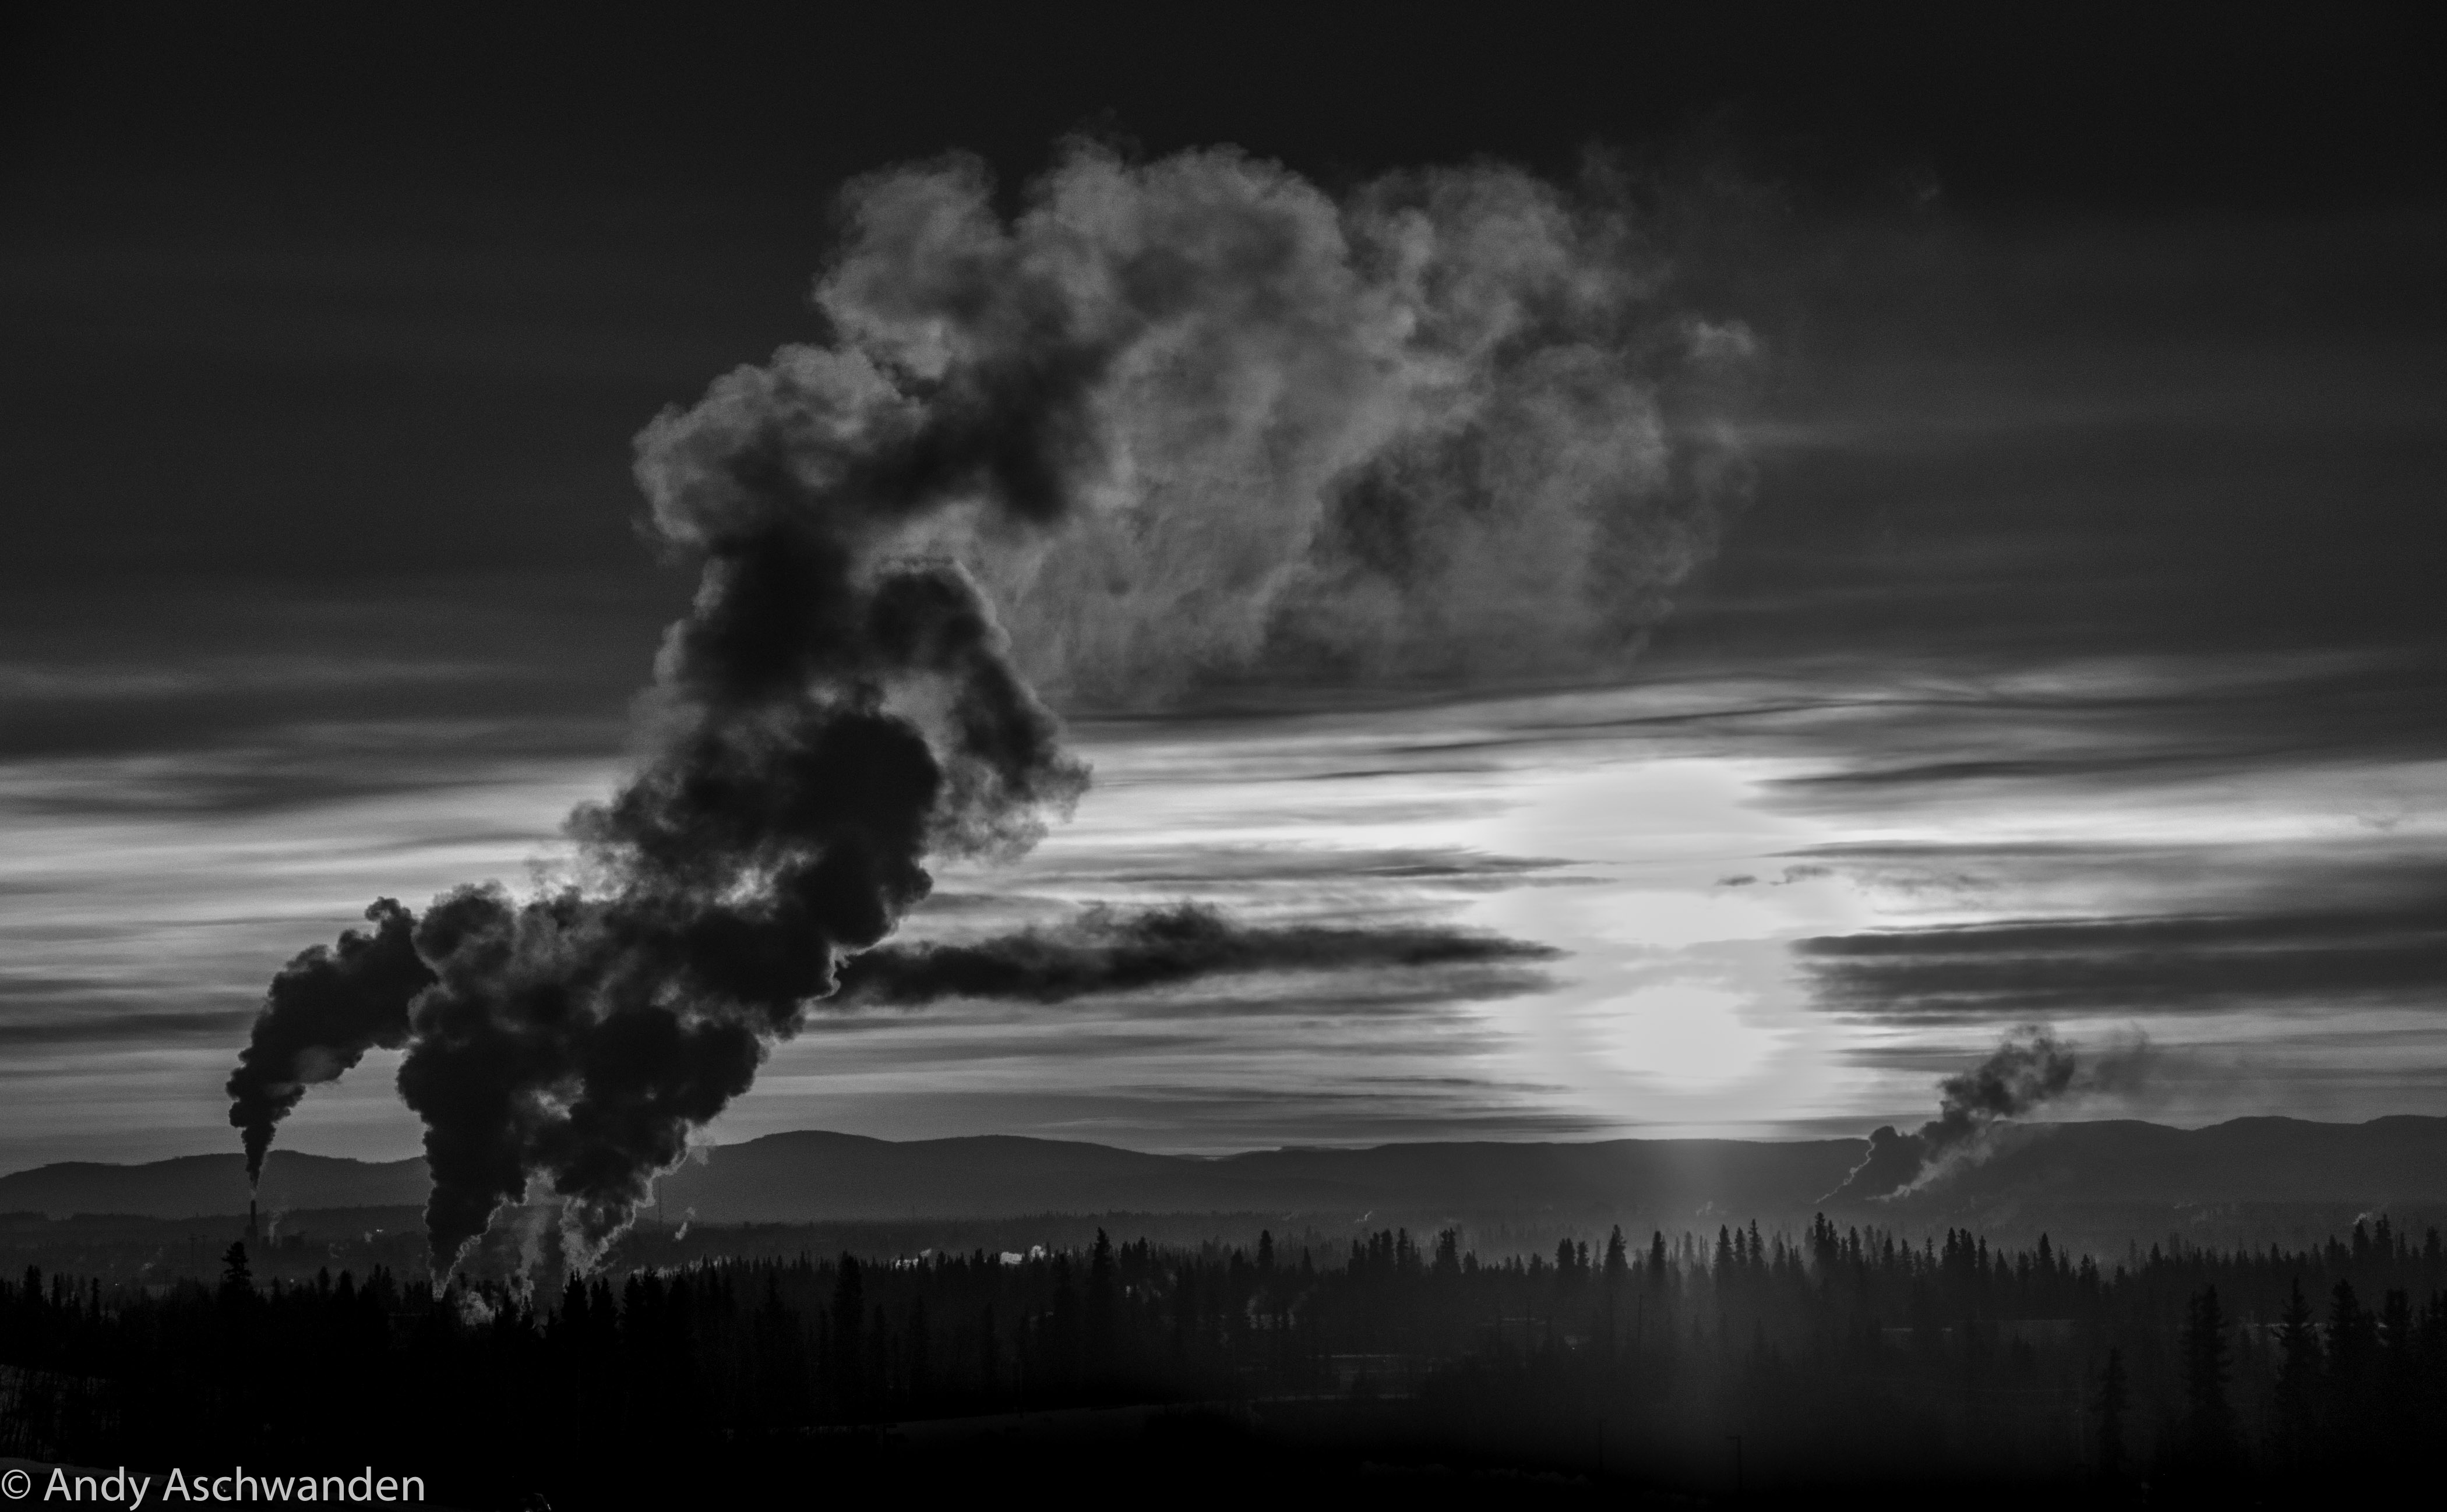
\includegraphics[height=\paperheight,width=\paperwidth]{uaf_power_plant}};}
} 

\begin{frame}[plain]
\end{frame}

\setbeamertemplate{background canvas}
  {
     \tikz{\node[inner sep=0pt,opacity=0.5] {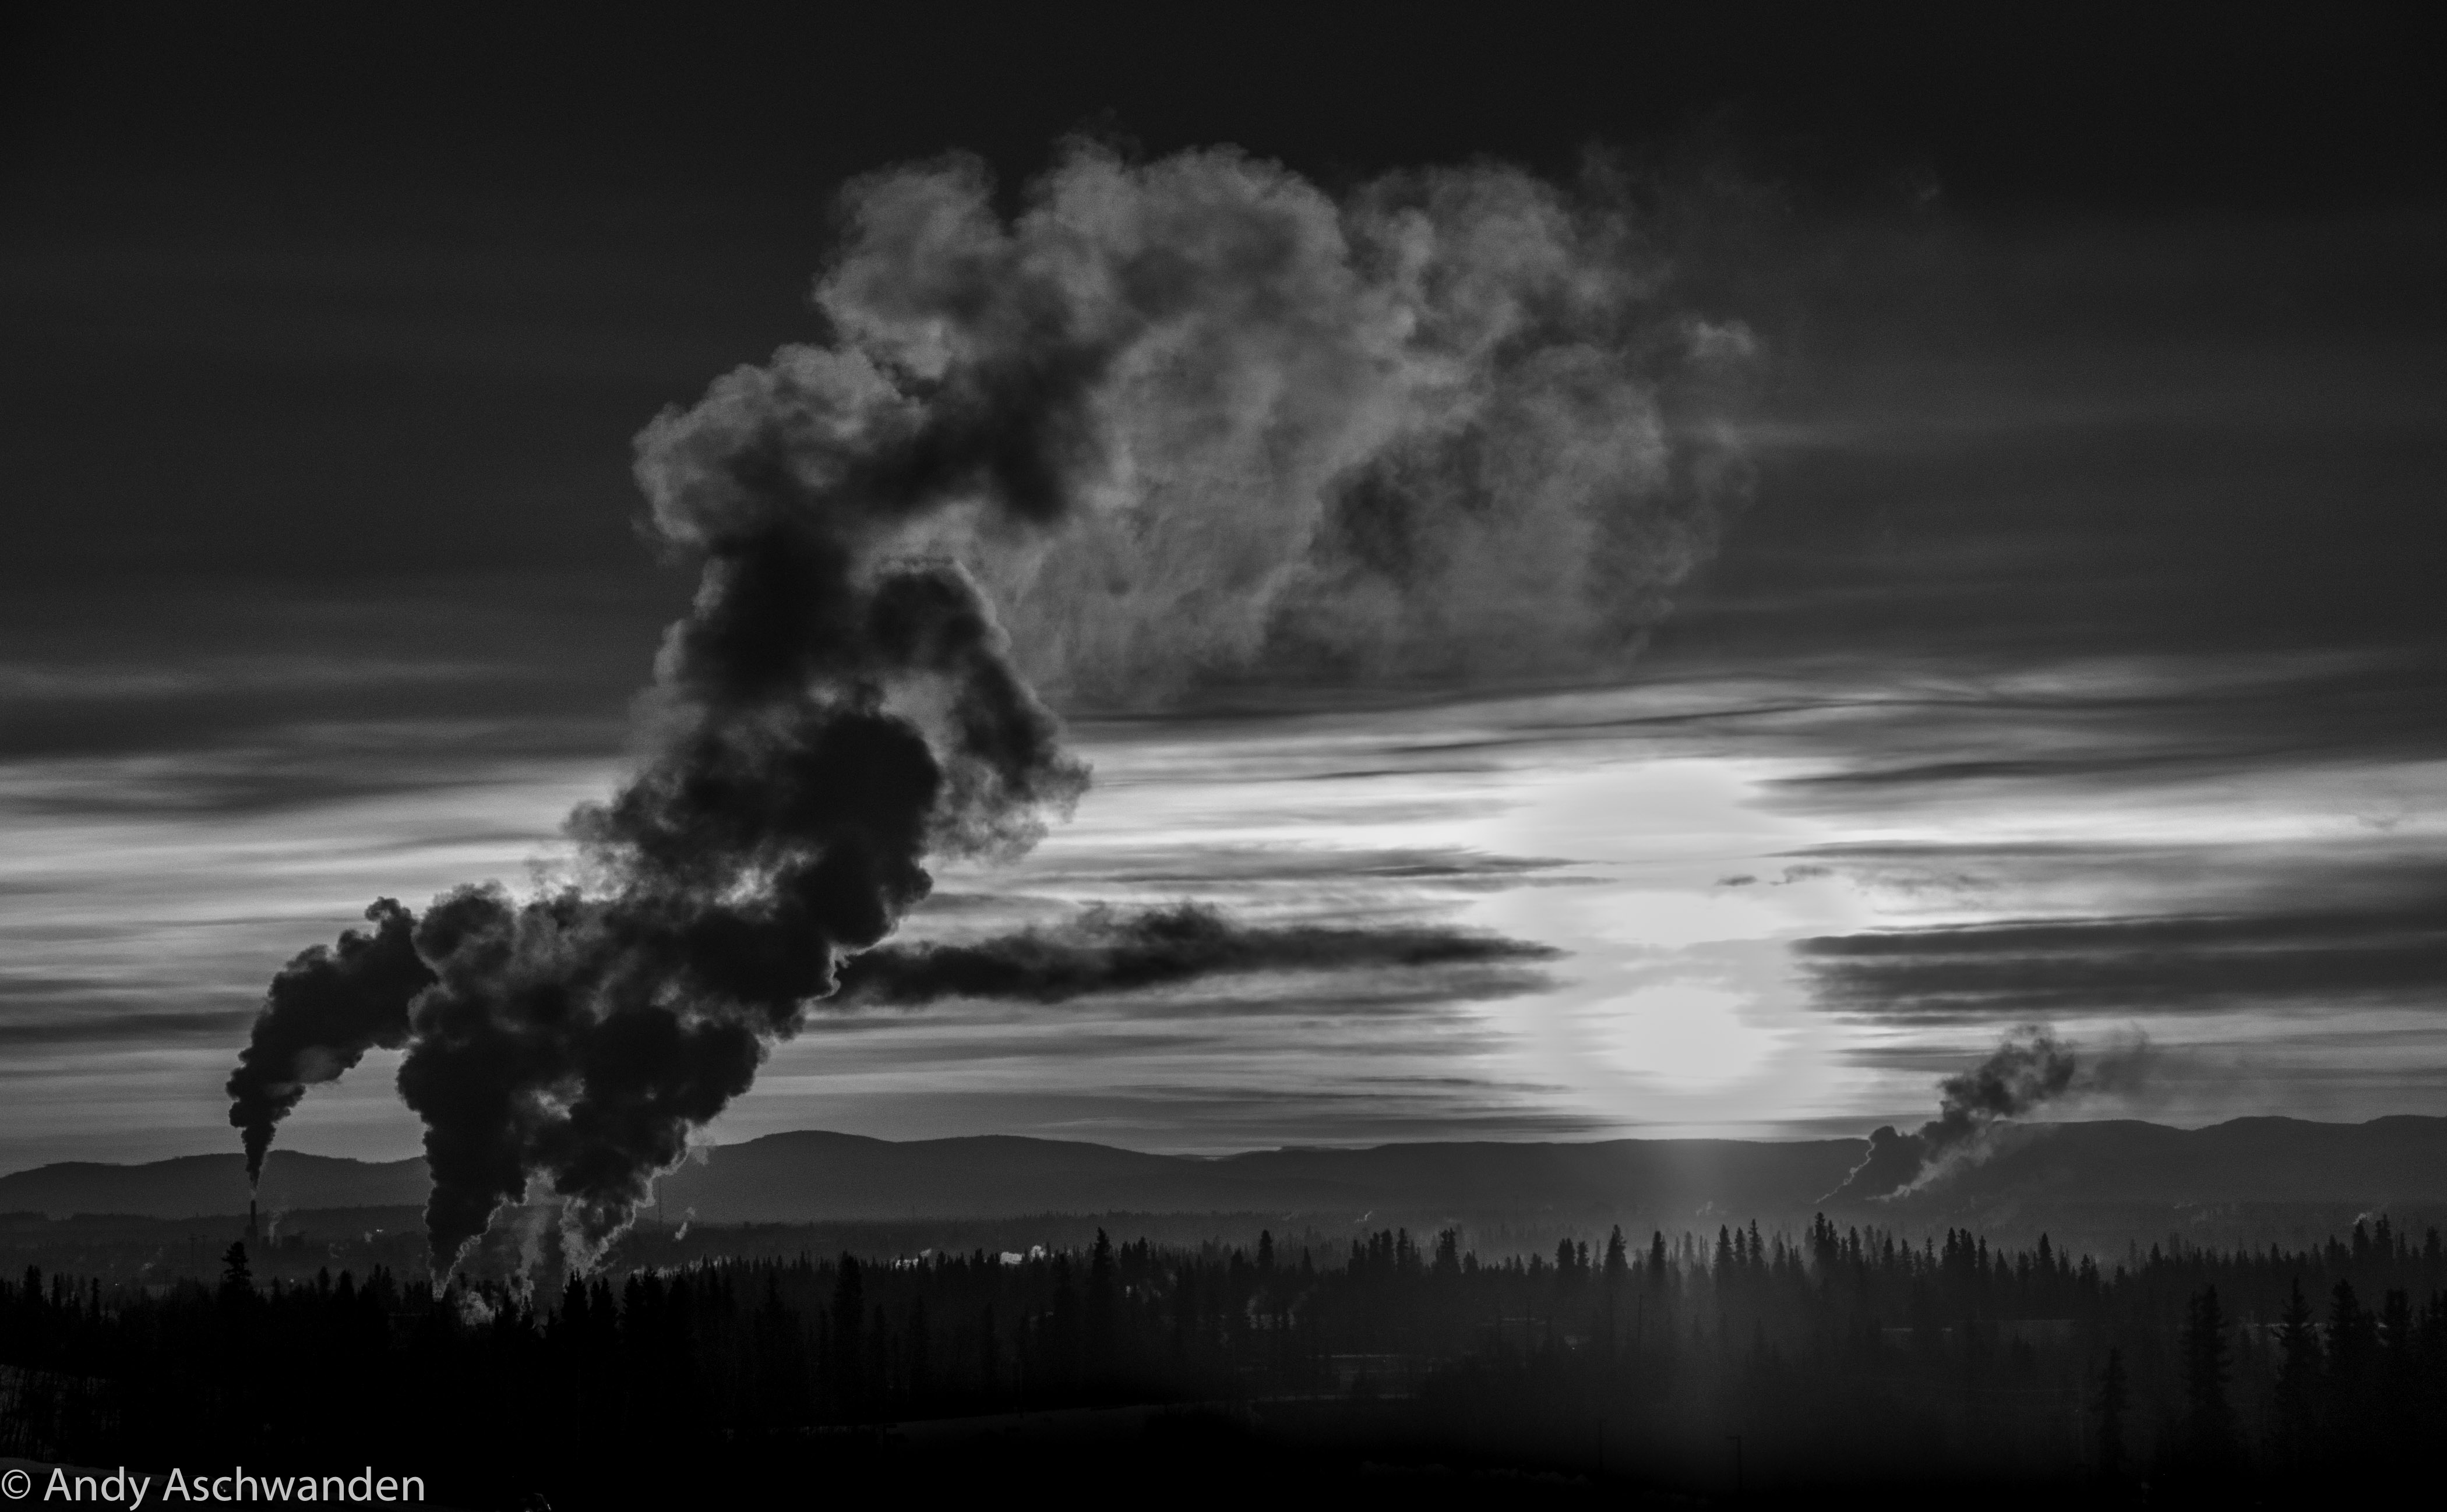
\includegraphics[height=\paperheight,width=\paperwidth]{uaf_power_plant}};}
} 

\begin{frame}[plain]
    \begin{itemize}
      \item Combustion of available fossil fuel resources sufficient to eliminate the Antarctic Ice Sheet (Winkelmann \emph{et al.}, 2015)
      \item this would raise sea level by 58\,m (plus another 7\,m from the Greenland Ice Sheet)
    \end{itemize}
\end{frame}


\setbeamertemplate{background canvas}
  {
     \tikz{\node[inner sep=0pt,opacity=1] {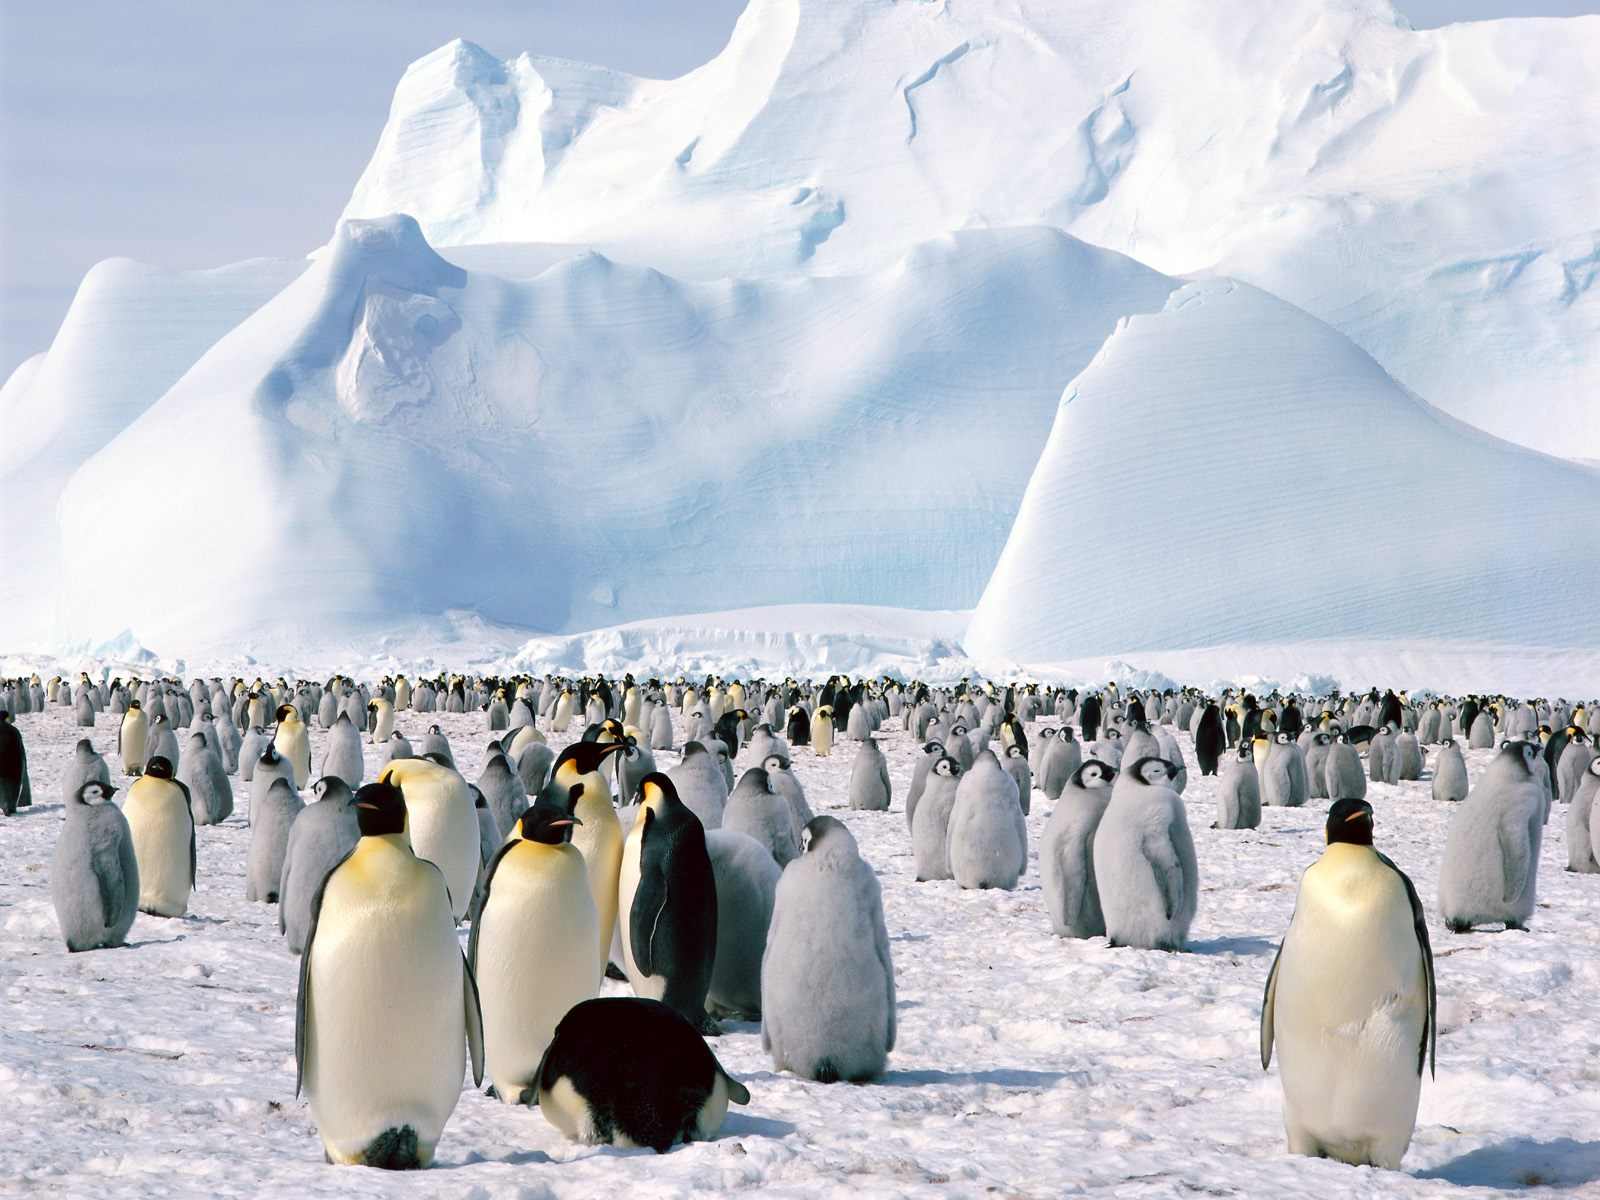
\includegraphics[height=\paperheight,width=\paperwidth]{ant_penguins}};}
} 

\begin{frame}[plain]
\end{frame}

\setbeamertemplate{background canvas}
  {
     \tikz{\node[inner sep=0pt,opacity=1] {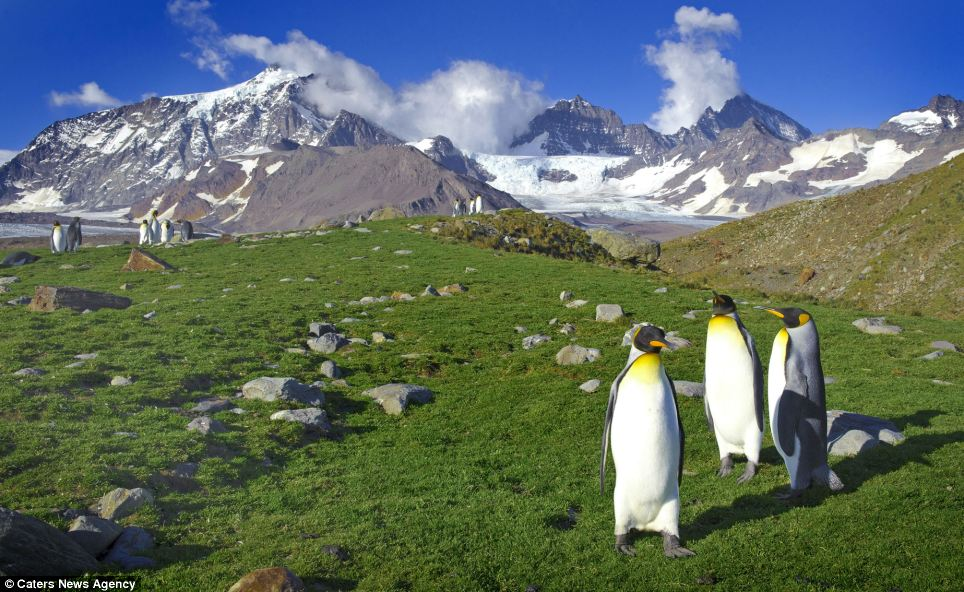
\includegraphics[height=\paperheight,width=\paperwidth]{green_penguins}};}
} 

\begin{frame}[plain]
\end{frame}



\setbeamertemplate{background canvas}
{
%
} 


\begin{frame}{How an ice sheet loses mass}
  \begin{figure}
    \includegraphics[width=\textwidth]{ice-sheet-cartoon}
  \end{figure}
  \note[item]{explain surface melt, ice discharge/calving, and basal melt}
  \note[item]{snow accumulates in the colder, higher altitude areas in the interior}
  \note[item]{turns into ice}
  \note[item]{and starts to flow downhill towards the coast}
  \note[item]{near the coast, surface melting can occur in the summer}
  \note[item]{but also some ice is dumped directly into the ocean}
  \note[item]{before the mid-90s mass loss was dominated by surface mass balance (80-90\%)}
  \note[item]{contribution of ice discharge was modest (10--20\%)}
  \note[item]{explaining in more detail in the next slide}
\end{frame}

\begin{frame}{Postitive feedsbacks}
(at least) two positive feedbacks accelerate mass loss
\begin{itemize}
\item with the climate (Bodvardsson effect)
\item geometrical instability (marine ice sheet hypothesis)
\end{itemize}
\end{frame}


\begin{frame}{Mountain Glacier}
 \begin{figure}
    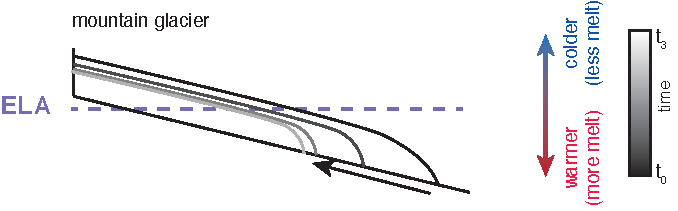
\includegraphics[width=\textwidth]{bodvardsson-effect_mountain_glacier}
  \end{figure}
\end{frame}

\begin{frame}{Ice Sheet}
 \begin{figure}
    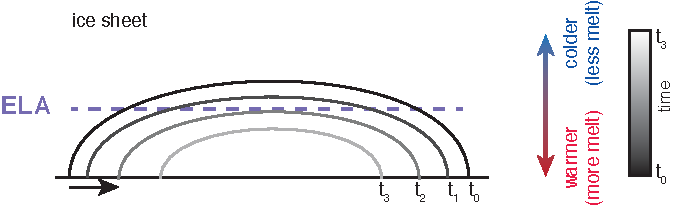
\includegraphics[width=\textwidth]{bodvardsson-effect_ice_sheet}
  \end{figure}
\end{frame}


\begin{frame}{Marine Ice Sheet Instability}
 \begin{figure}
    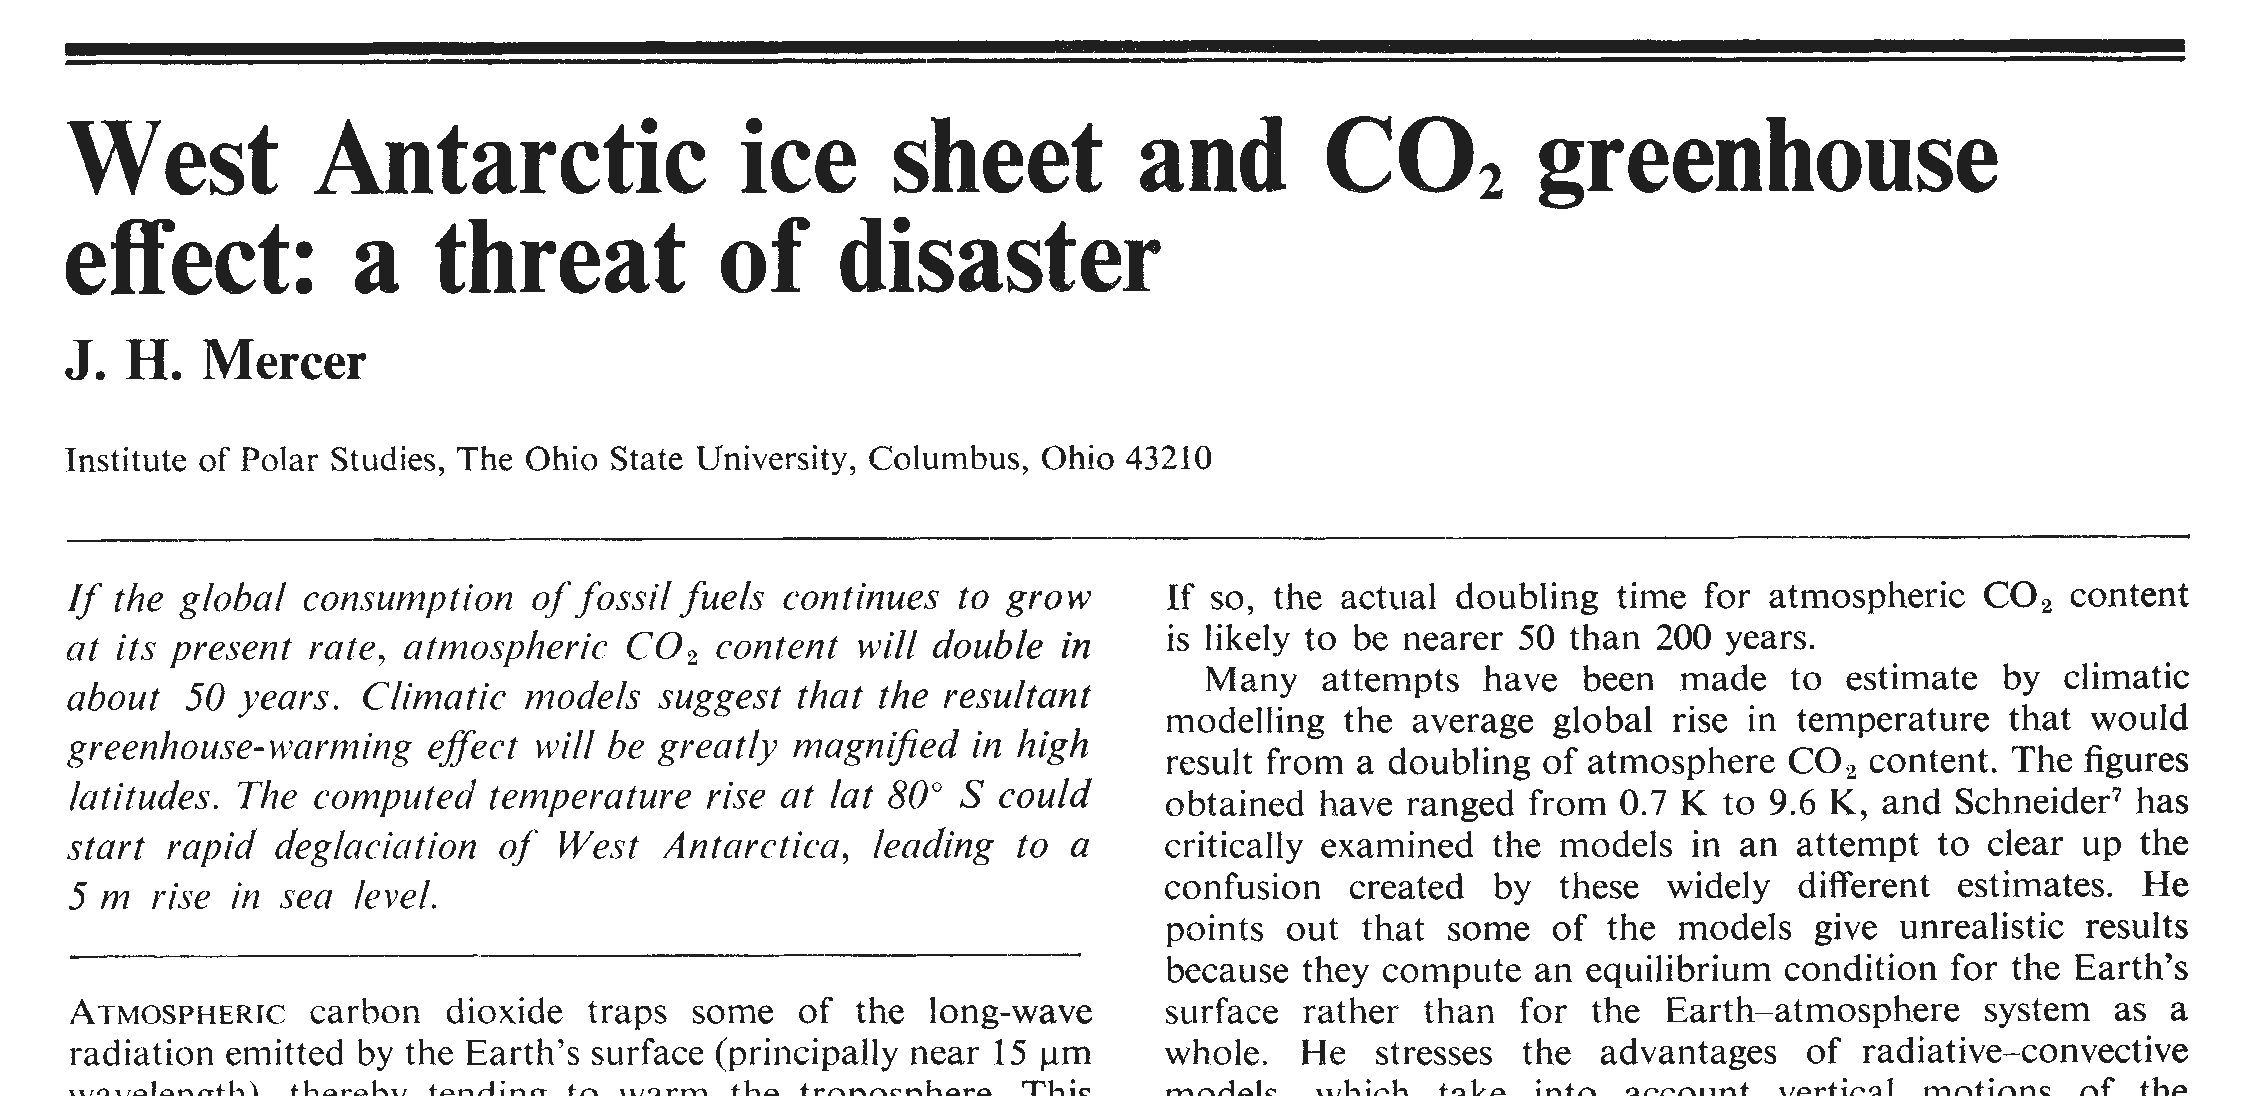
\includegraphics[width=\textwidth]{mercer_1978}
  \end{figure}
\end{frame}

\begin{frame}{Marine Ice Sheet Instability}
 \begin{figure}
    \includegraphics[height=8cm]{ant-marine}
  \end{figure}
\end{frame}

\setbeamertemplate{background canvas}
  {
     \tikz{\node[inner sep=0pt,opacity=.75] {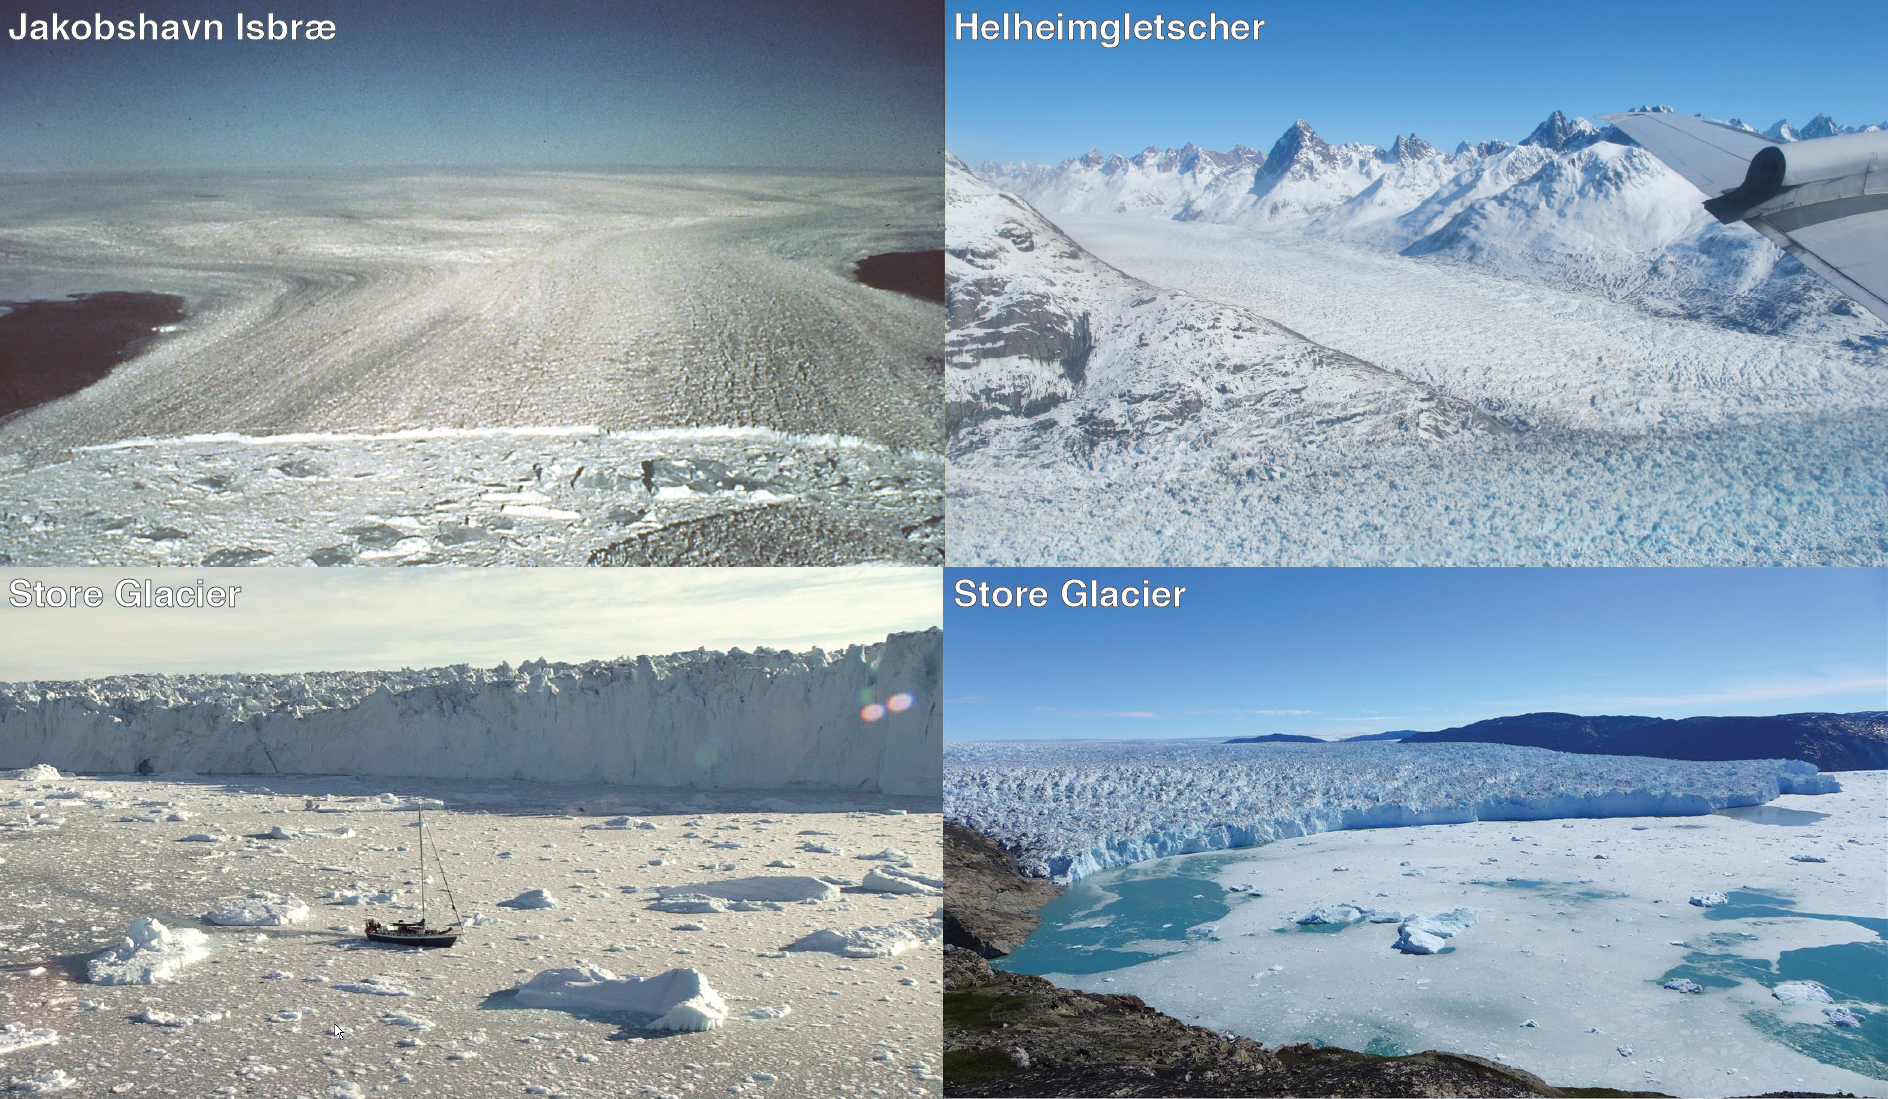
\includegraphics[height=\paperheight,width=\paperwidth]{outlet-glacier-collage-01}};}
}

\begin{frame}[plain]
  \textbf{In Greenland}
    \begin{itemize}
    \item ice discharge to the ocean occurs through 200+ ``outlet glaciers''
    \item outlet glaciers are flowing fast ($>$200\,m/yr), are controlled by bedrock geometry, and terminate in narrow fjords ($\sim <$10\,km wide)
    \end{itemize}
    \note[item]{outlet glaciers look pretty spectacular}
\end{frame}
 

\setbeamertemplate{background canvas}
  {
     \tikz{\node[inner sep=0pt,opacity=1] {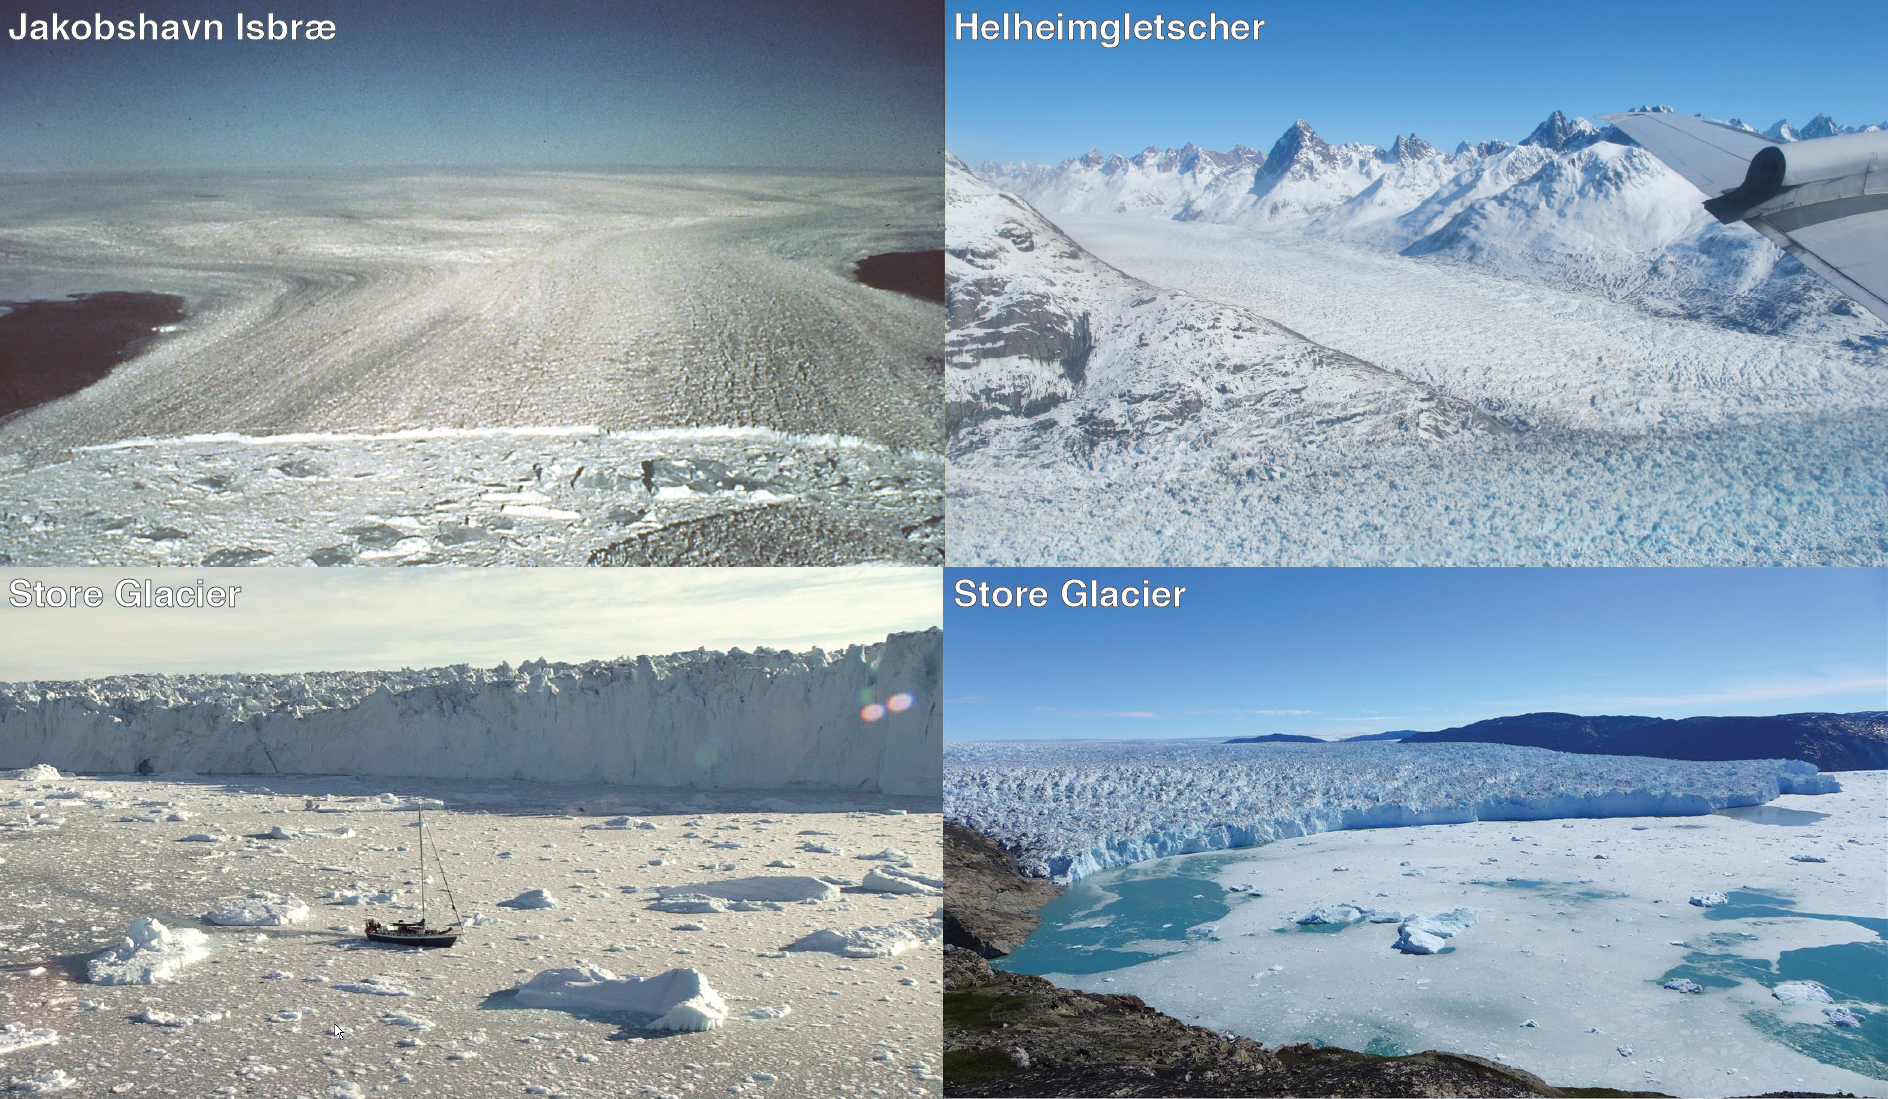
\includegraphics[height=\paperheight,width=\paperwidth]{outlet-glacier-collage-01}};}
}

\begin{frame}[plain]
  \note[item]{some very passionate glaciologists get really close to the terminus in their sailing boats}
\end{frame}


\setbeamertemplate{background canvas}
  {
     \tikz{\node[inner sep=0pt,opacity=1] {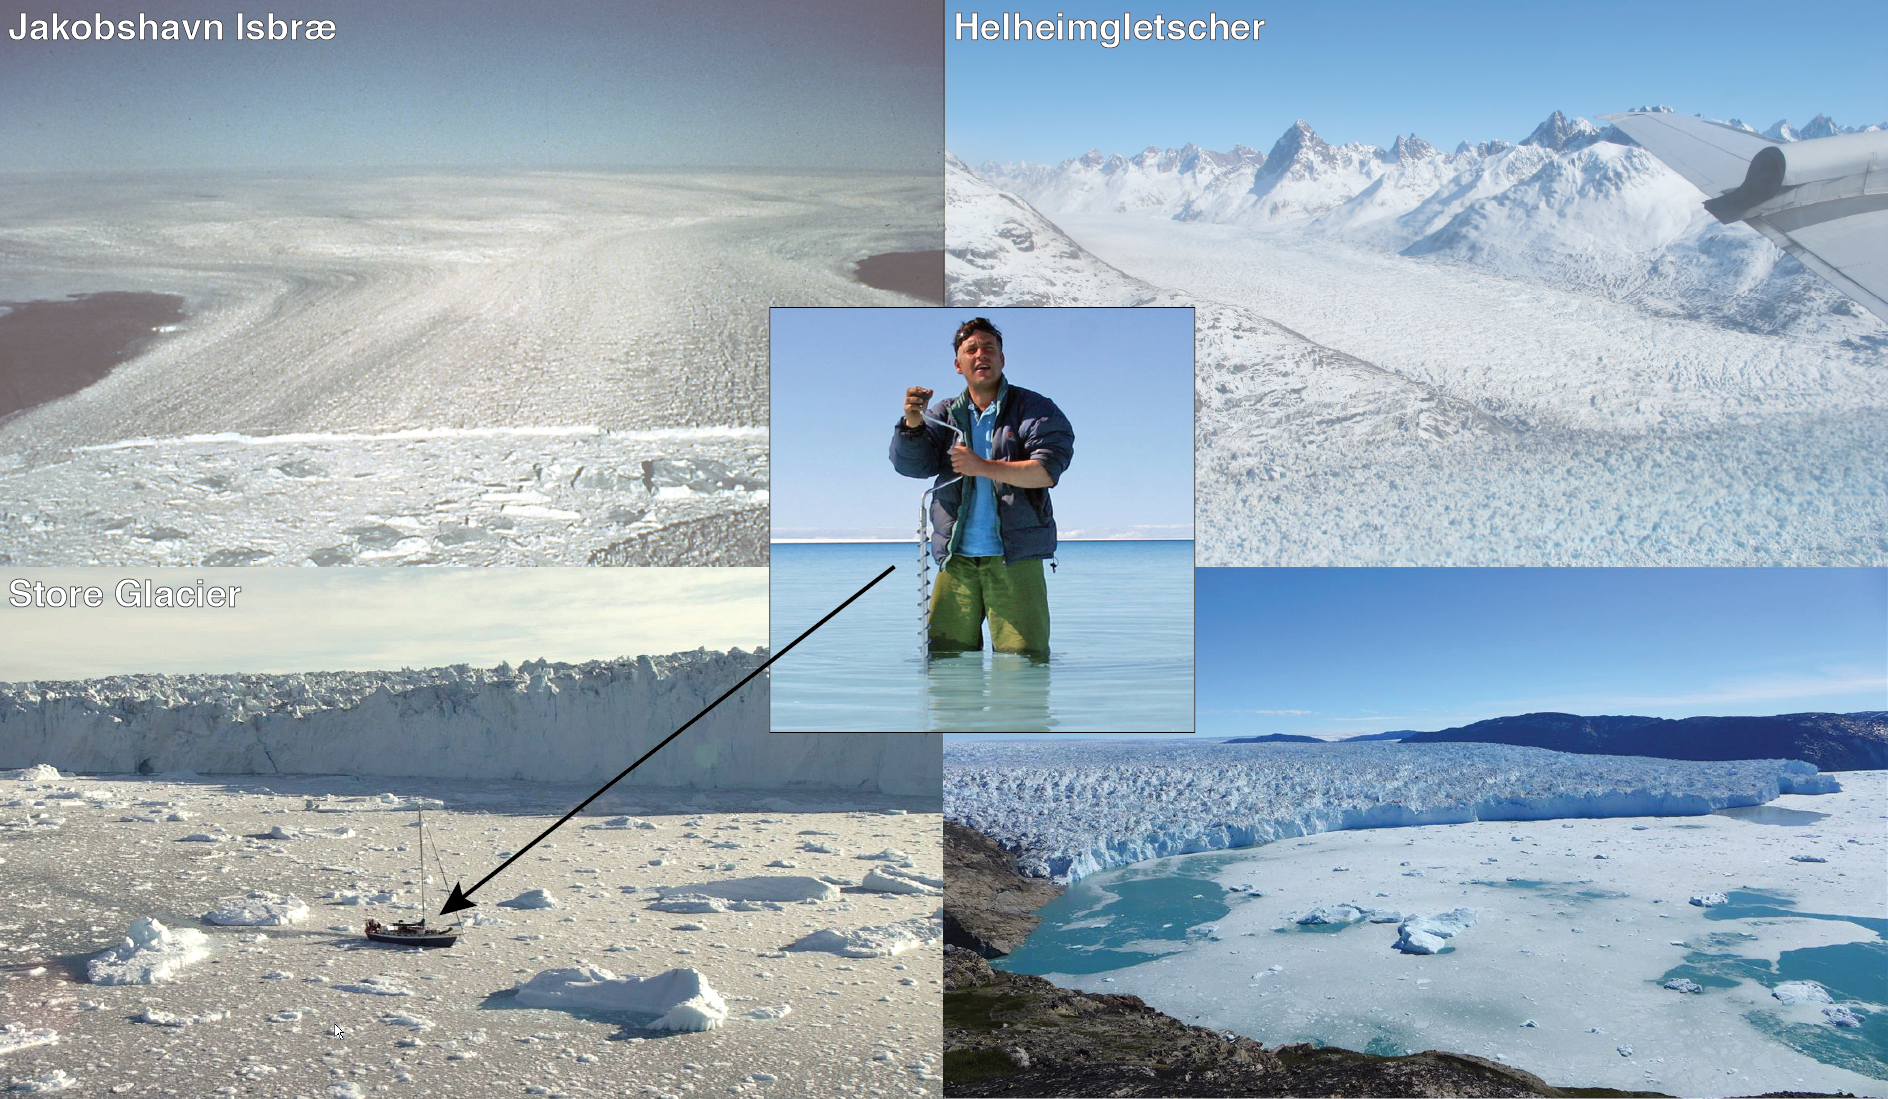
\includegraphics[height=\paperheight,width=\paperwidth]{outlet-glacier-collage-alun-01}};}
}

\begin{frame}[plain]
  \note[item]{some very passionate glaciologists get really close to the terminus in their sailing boats}
\end{frame}



\setbeamertemplate{background canvas}
{
%
} 


\begin{frame}{Jakobshavn Isbr{\ae}, west Greenland}
 \begin{figure}
    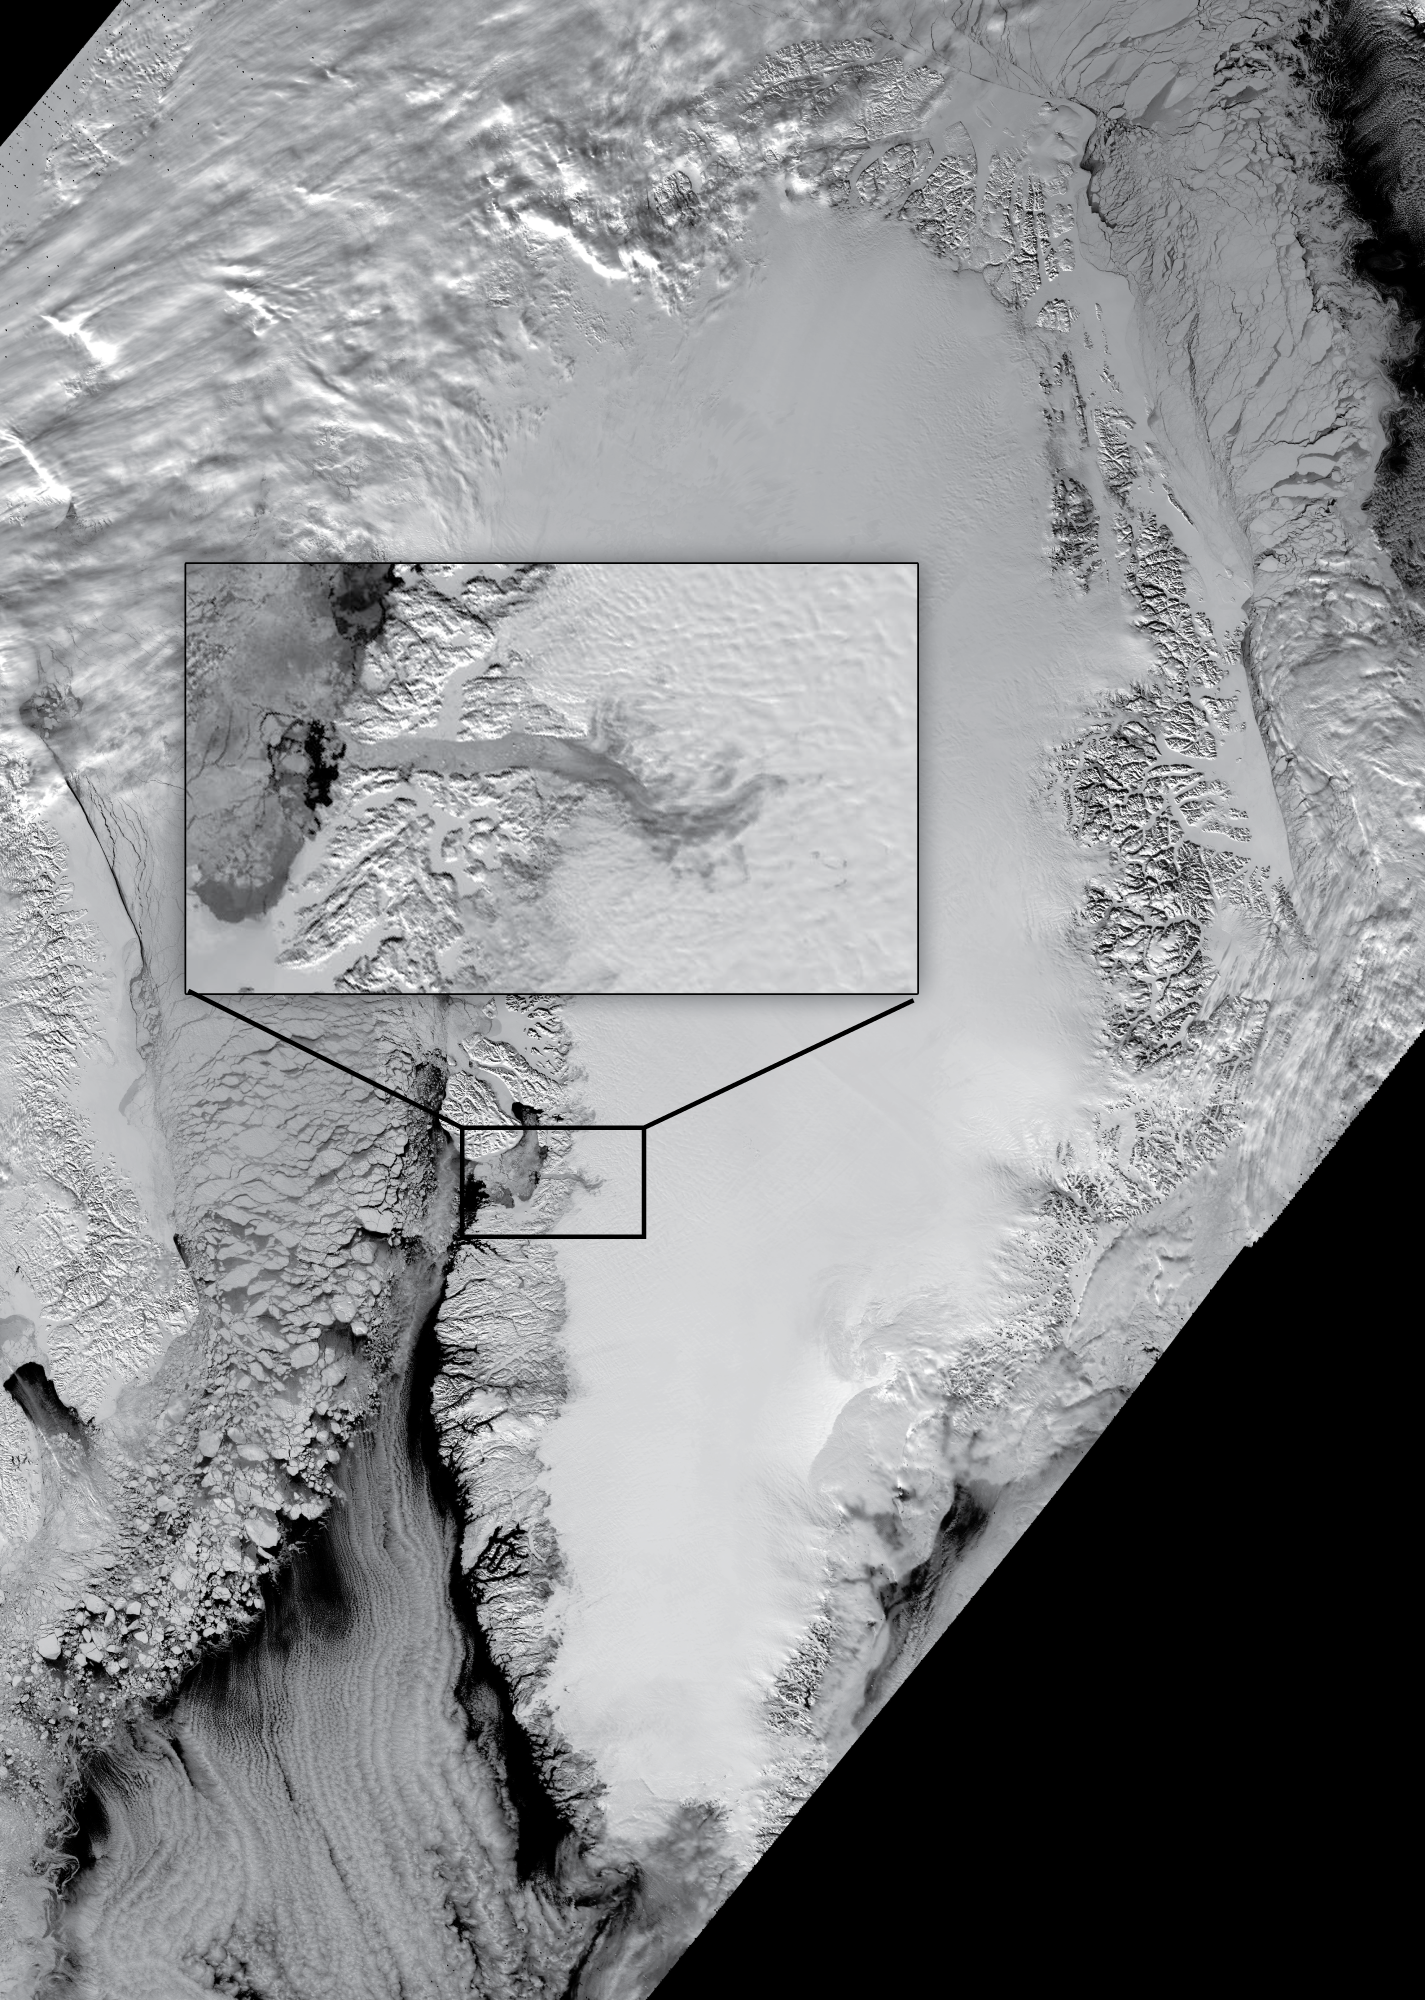
\includegraphics[height=.8\textheight]{MODISGreenlandJakobshavn} \\
    \scriptsize{based on MODIS data from M. Fahnestock}
  \end{figure}
  \note[item]{in this talk I will focus on Jakobshavn}
  \note[item]{Greenland's biggest and fastest flowing outlet glacier}
  \note[item]{drains about 7\% of the entire ice sheet}
\end{frame}


\begin{frame}{A short history}
 \begin{figure}
    \includegraphics[width=\textwidth]{Jakobshavn_groundline_retreat} \\
  \end{figure}
  \note[item]{Will Harrison and late Keith Echelmeyer investigated Jakobshavn in the mid-80s}
  \note[item]{at that time JIB had a $\sim$10\,km long floating tongue}
  \note[item]{they found high flow speeds}
  \note[item]{relatively steady behavior}
  \note[item]{in 1997, the glacier suddenly switched from slow thickening to rapid thinning}
  \note[item]{caused by an increase in subsurface ocean temperature from 1.7degC in 1995 to 3.3degC in 1998, leading to increased melting}
  \note[item]{In summer 1998 the first major increase in surface velocity was seen}
  \note[item]{first departure from the normal pattern of frontal positions 1998}
  \note[item]{retreat of the ice front started around 2002}
\end{frame}


\begin{frame}{Frontal retreat 1990--2005}
 \begin{figure}
    \includegraphics<1>[width=\textwidth]{jib-front-1990}
    \includegraphics<2>[width=\textwidth]{jib-front-1990-floating}
    \includegraphics<3>[width=\textwidth]{jib-front-2005}
    \includegraphics<4>[width=\textwidth]{jib-front-1990-2005-change}
    \includegraphics<5>[width=\textwidth]{jib-front-1990-2005-plug}
  \end{figure}
  \note[item]{the loss of the floating tongue is what I'm calling pulling the plug}
  \note[item]{exact timing of the break-up remains elusive due to poor satellite coverage at that time}
\end{frame}


\begin{frame}{When you pull the plug: speed-up 1992-2000}
  \begin{itemize}
    \item almost doubled its flow speed between the 1992 and 2000
    \item slow but steady increase since then
  \end{itemize}
  \begin{figure}
    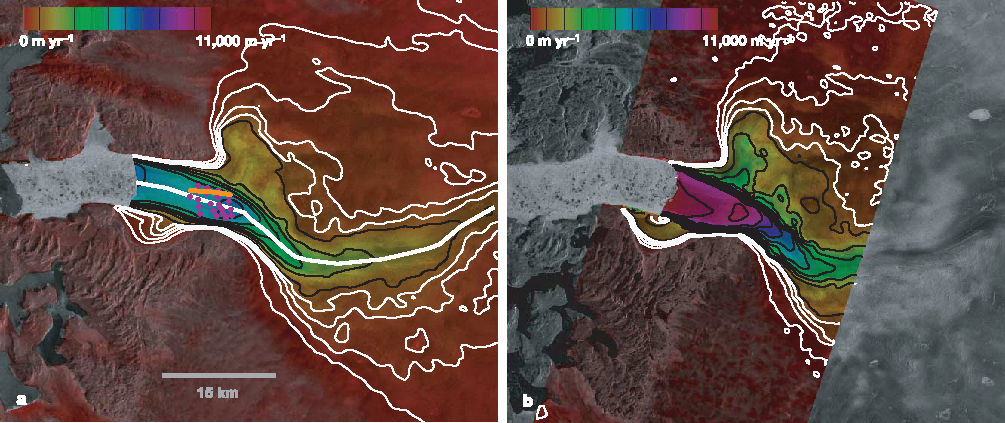
\includegraphics[width=\textwidth]{Joughin2004Fig2} \\
    \footnotesize{Joughin et al. (2004)}
  \end{figure}
  \note[item]{illustration of the speed up}
\end{frame}


\setbeamertemplate{background canvas}
  {
     \tikz{\node[inner sep=0pt,opacity=0.8] {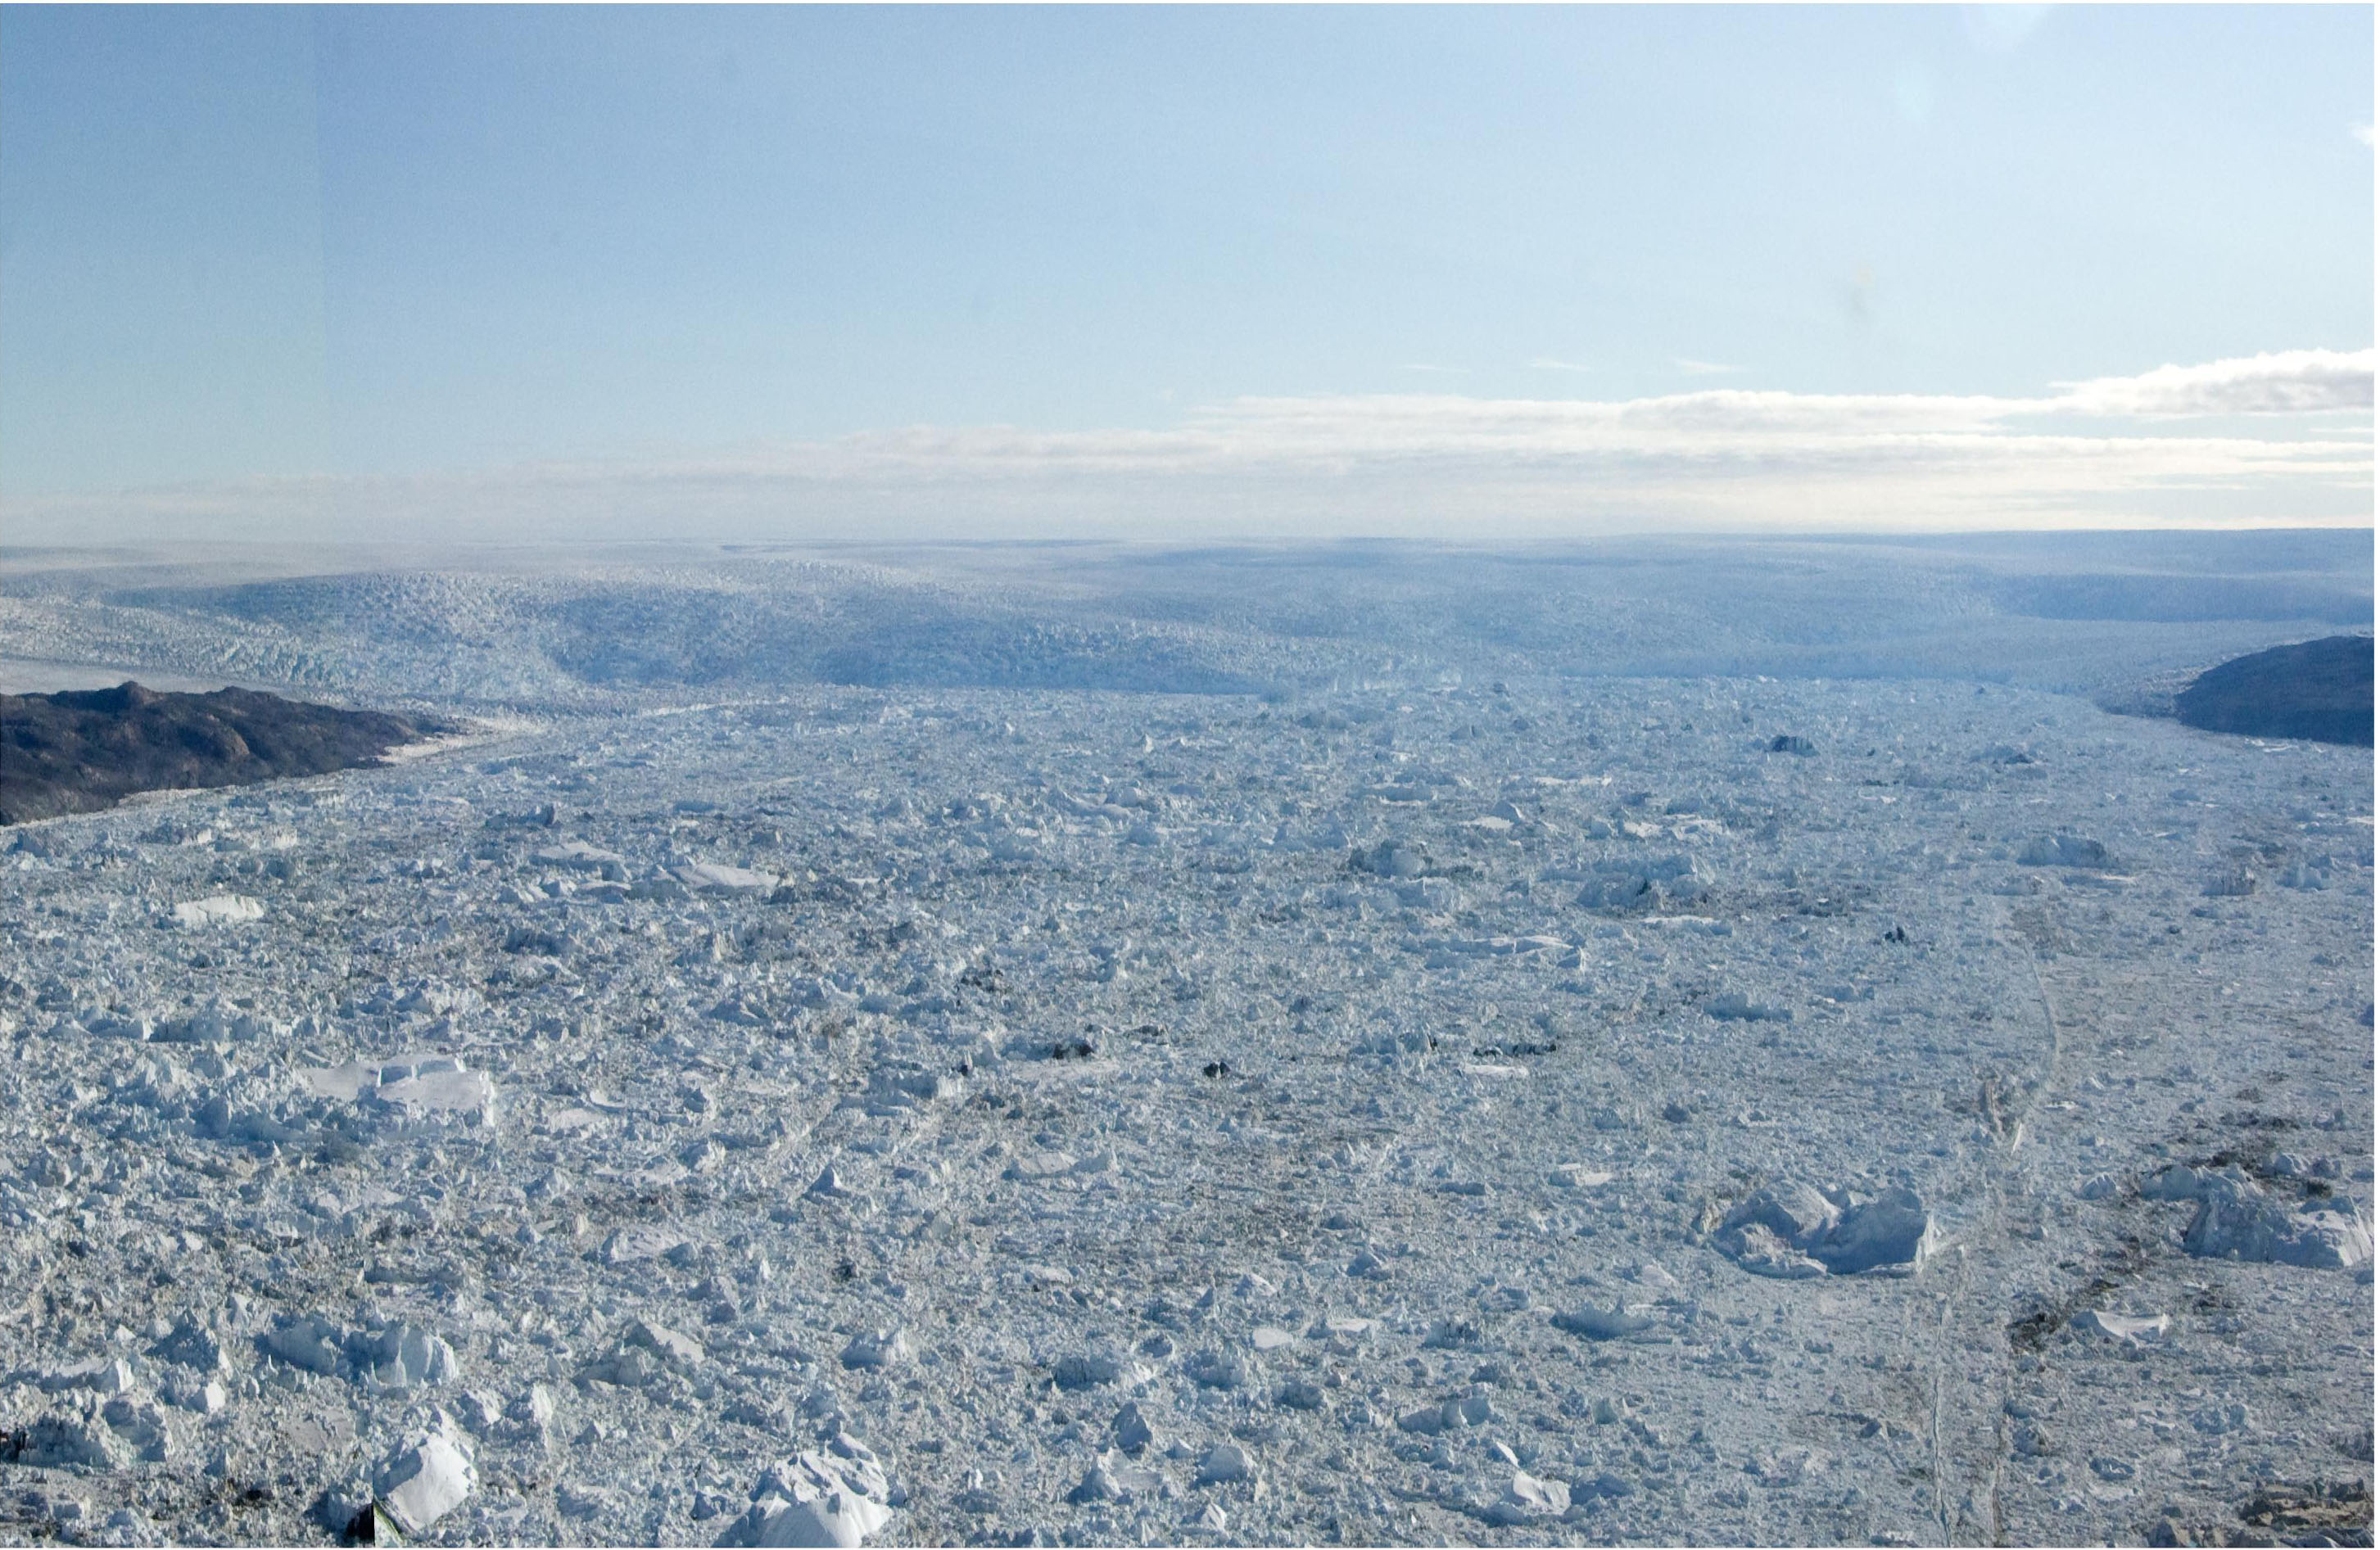
\includegraphics[height=\paperheight,width=\paperwidth]{jakobshavn-2007}};}
}


\begin{frame}{When you pull the plug: changes in ice discharge 2000-2010}
  \begin{itemize}
  \item increase in discharge from 40\,Gt/yr in 2000 to $\sim$60\,Gt/yr in 2010
  \item compared to $\sim$75\,Gt/yr total mass loss from all Alaskan glaciers
  \end{itemize}
  \note[item]{illustration of the speed up}
\end{frame}


\setbeamertemplate{background canvas}
{
%
} 

\begin{frame}{When you pull the plug: surface elevation changes 1985-2007}

  \begin{figure}
    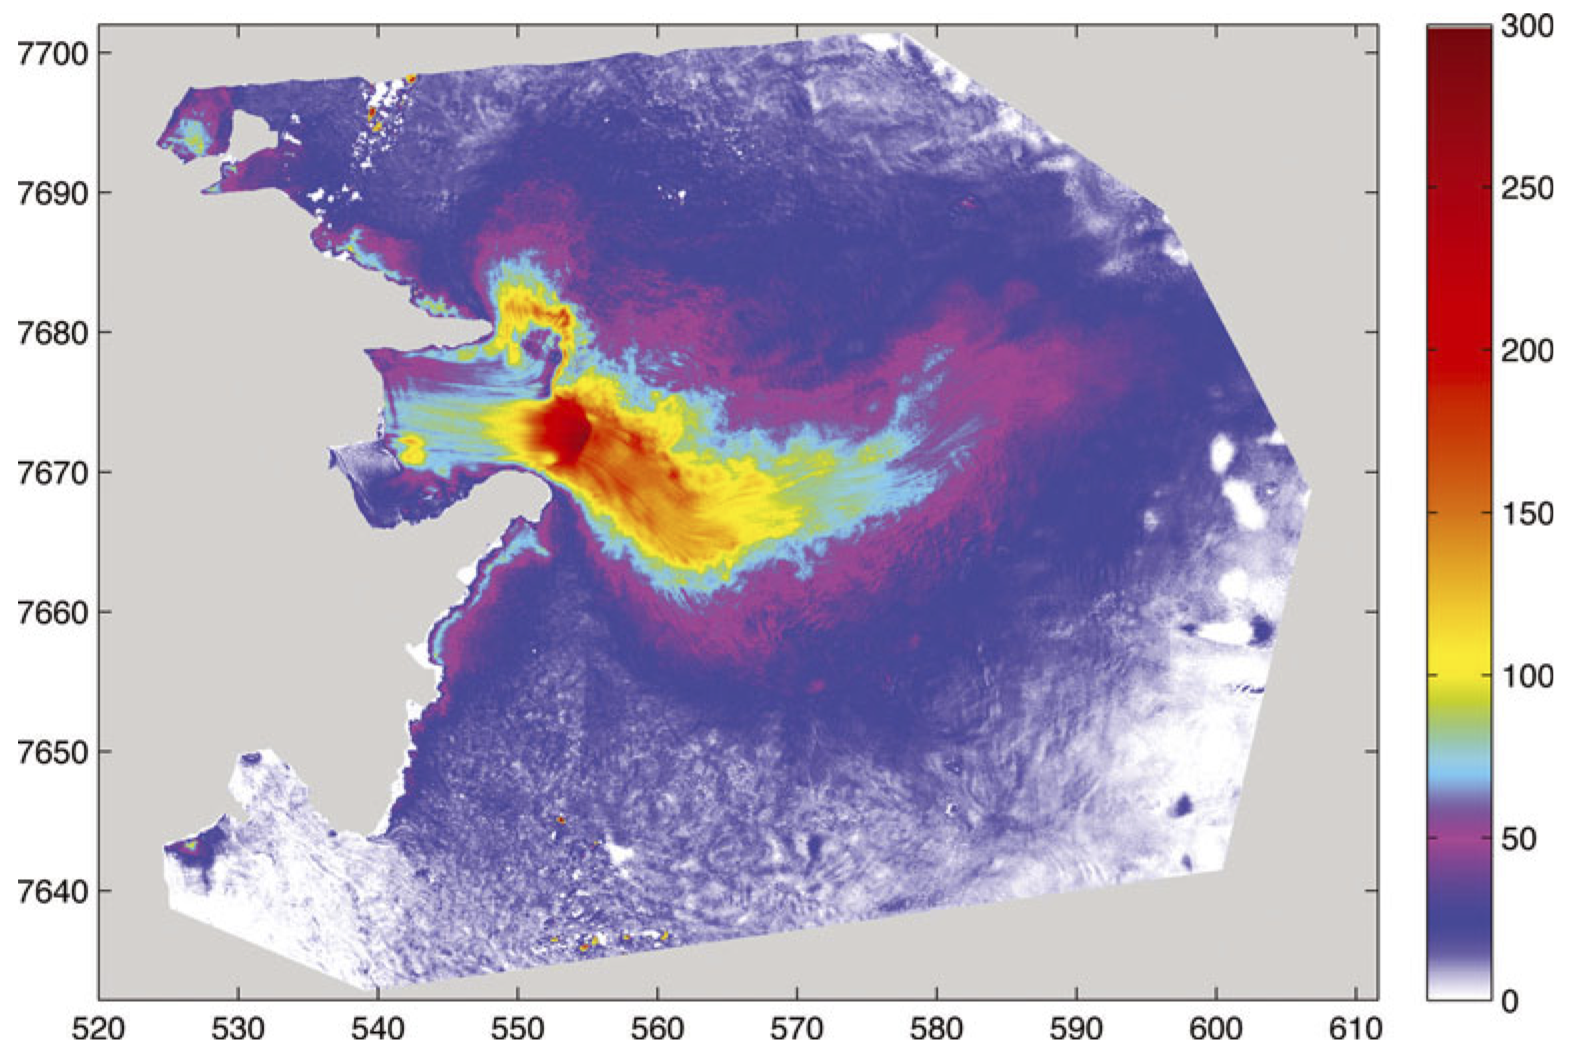
\includegraphics[width=.8\textwidth]{jib-obs-surface-diff-motyka} \\
    \footnotesize{Motyka, Fahnestock, Truffer (2010)}
  \end{figure}
  \note[item]{as a consequence of the increased discharge, the ice surface is drawing down near the glacier terminus}
\end{frame}


\begin{frame}{How can we reconcile/understand these changes?}
 \begin{figure}
    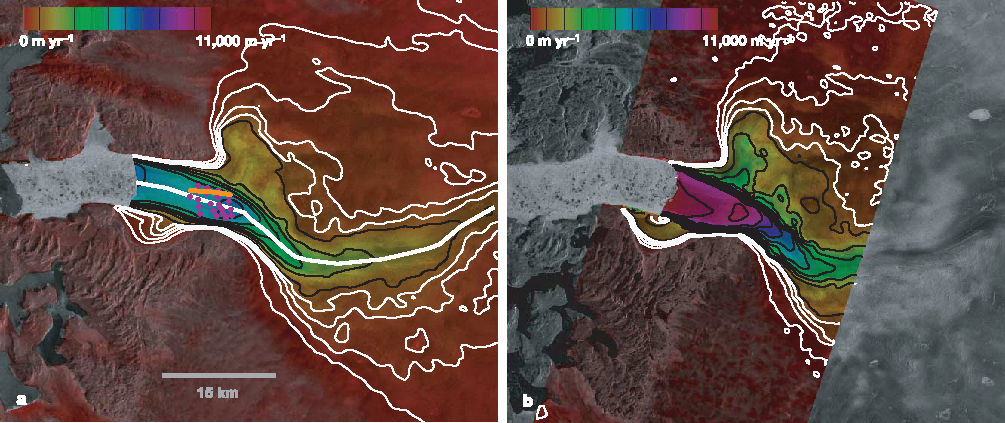
\includegraphics[height=4.15cm]{Joughin2004Fig2} \\
    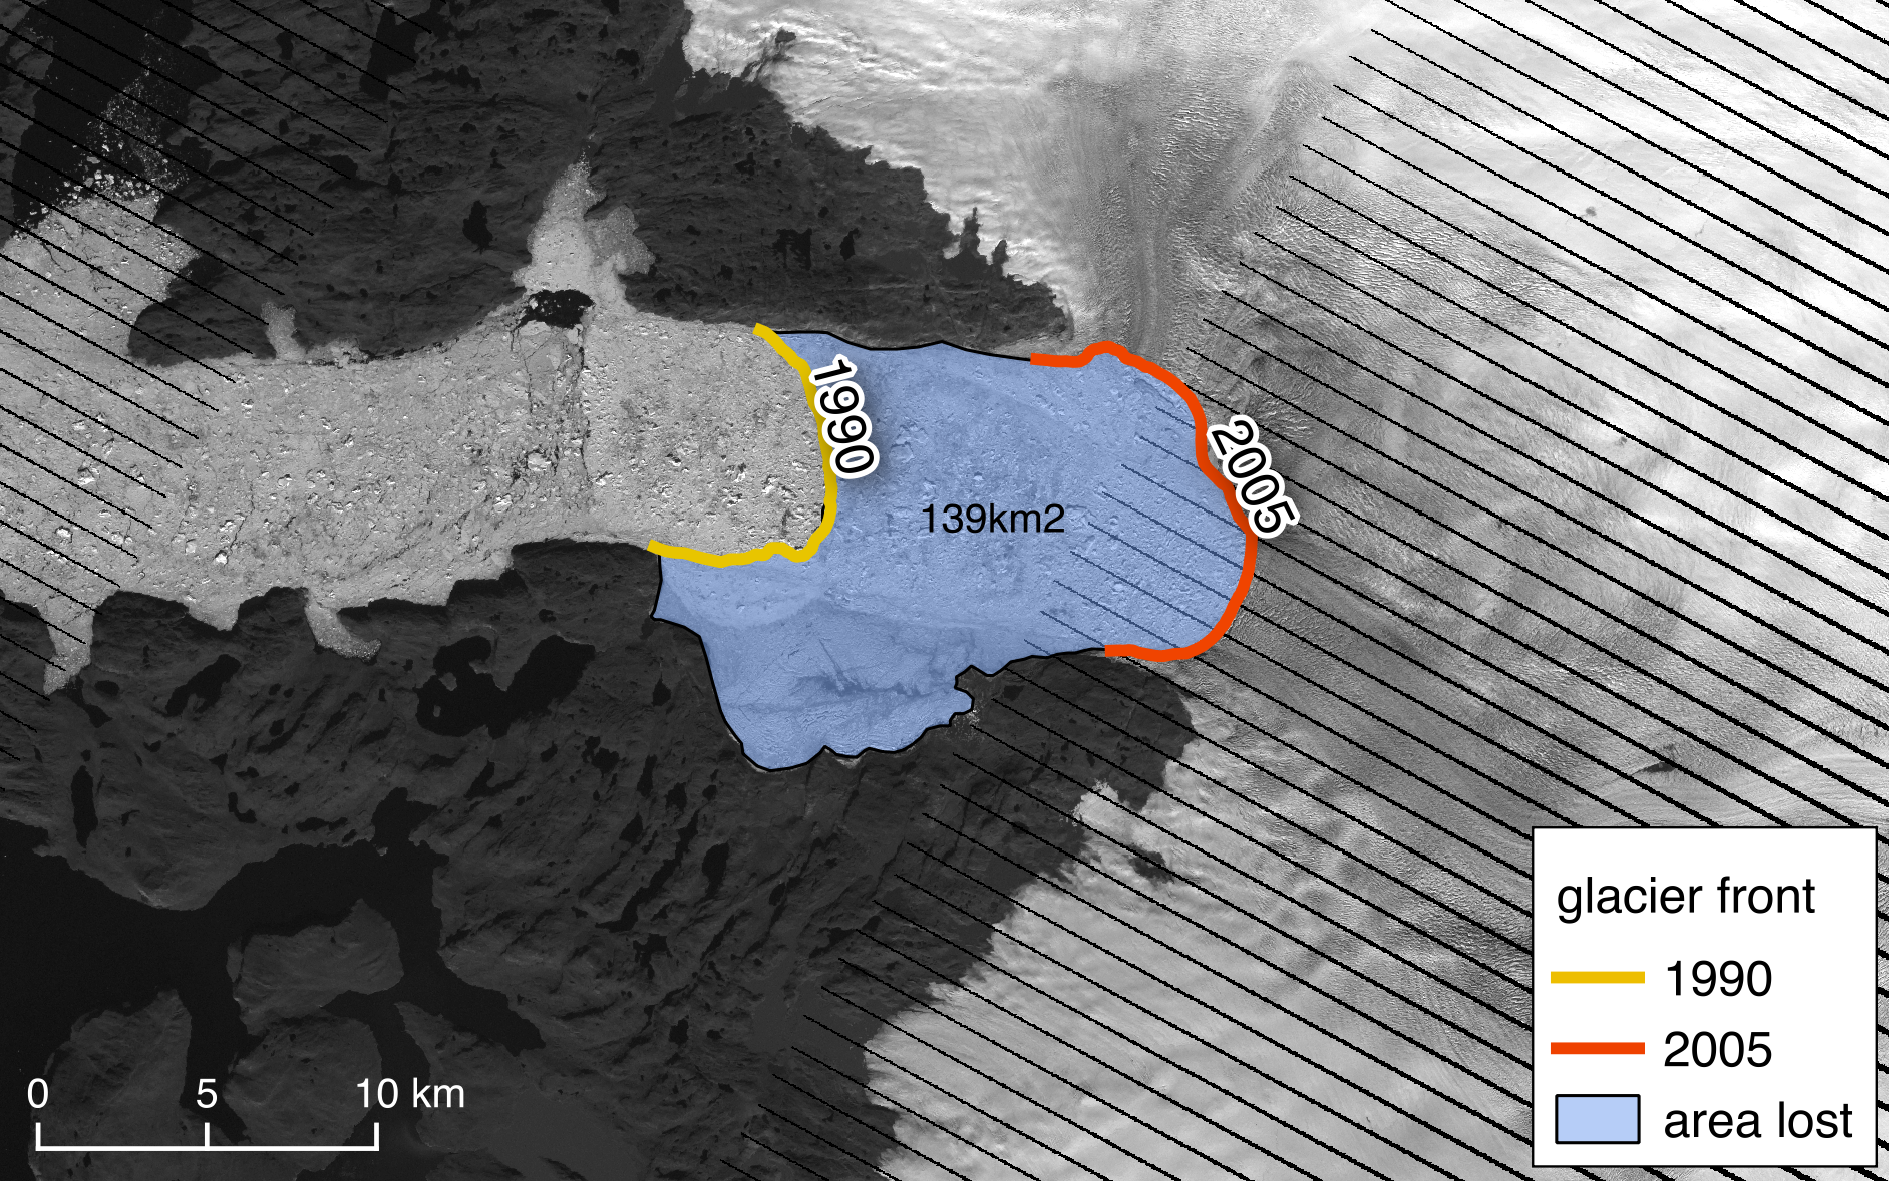
\includegraphics[height=3.20cm]{jib-front-1990-2005-change}
    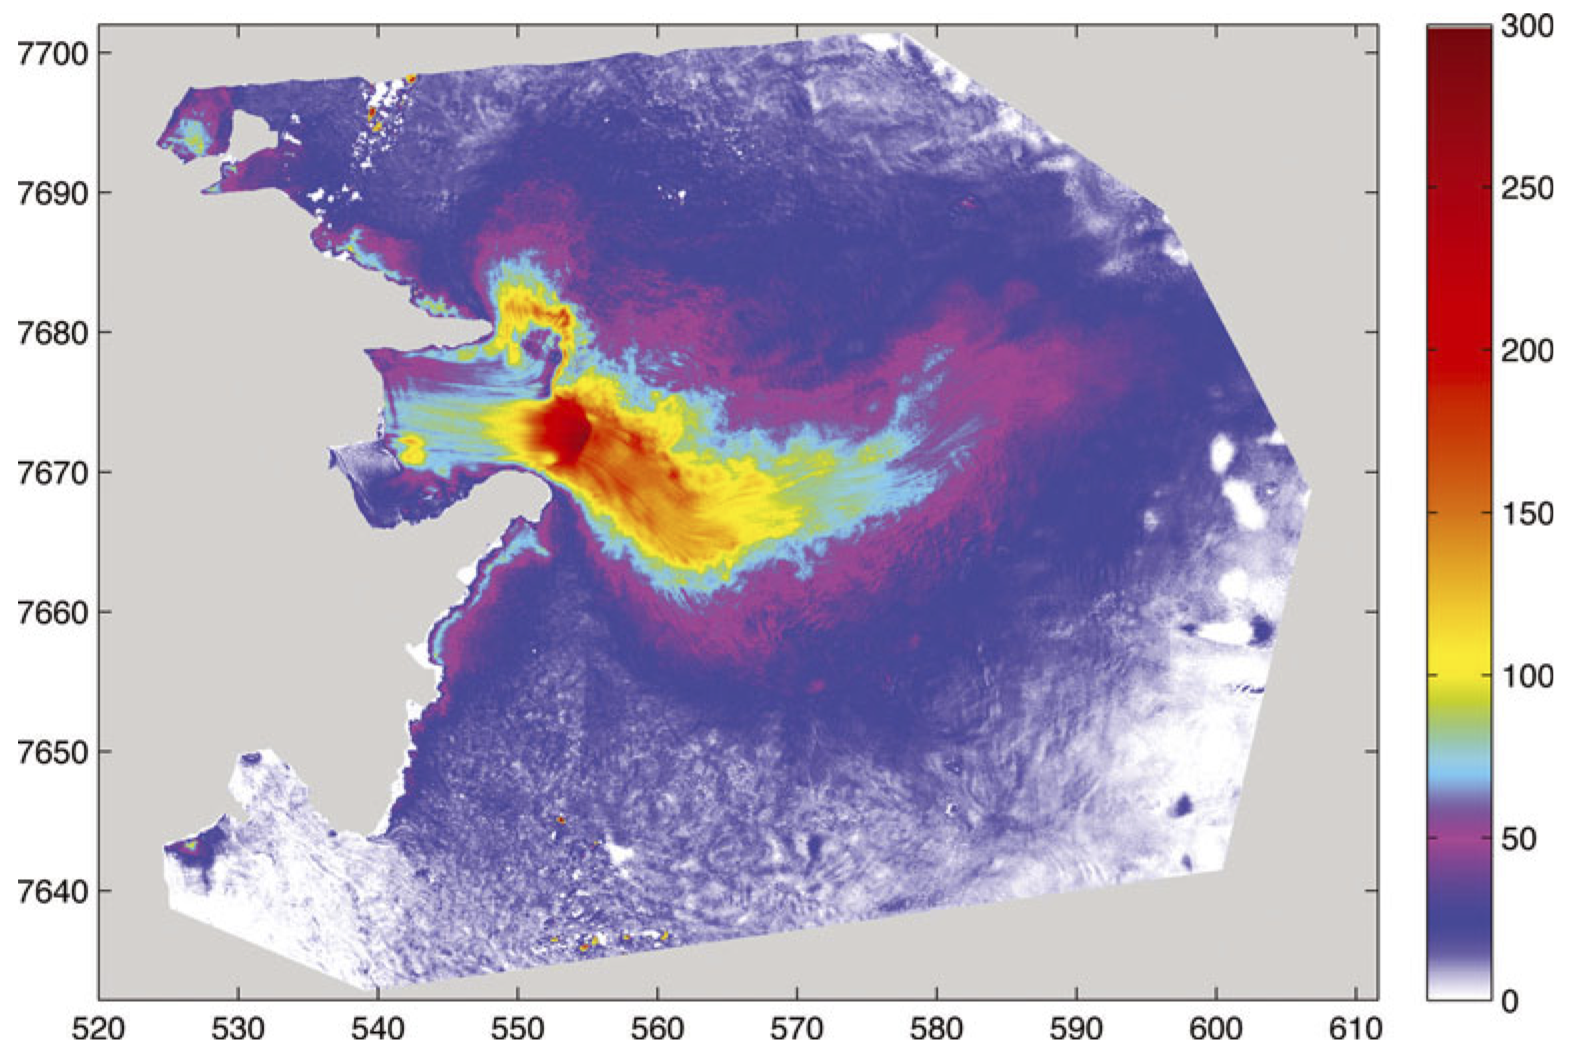
\includegraphics[height=3.20cm]{jib-obs-surface-diff-motyka}
  \end{figure}
\end{frame}


\begin{frame}{Answer: use an ice sheet model}
  \begin{figure}
    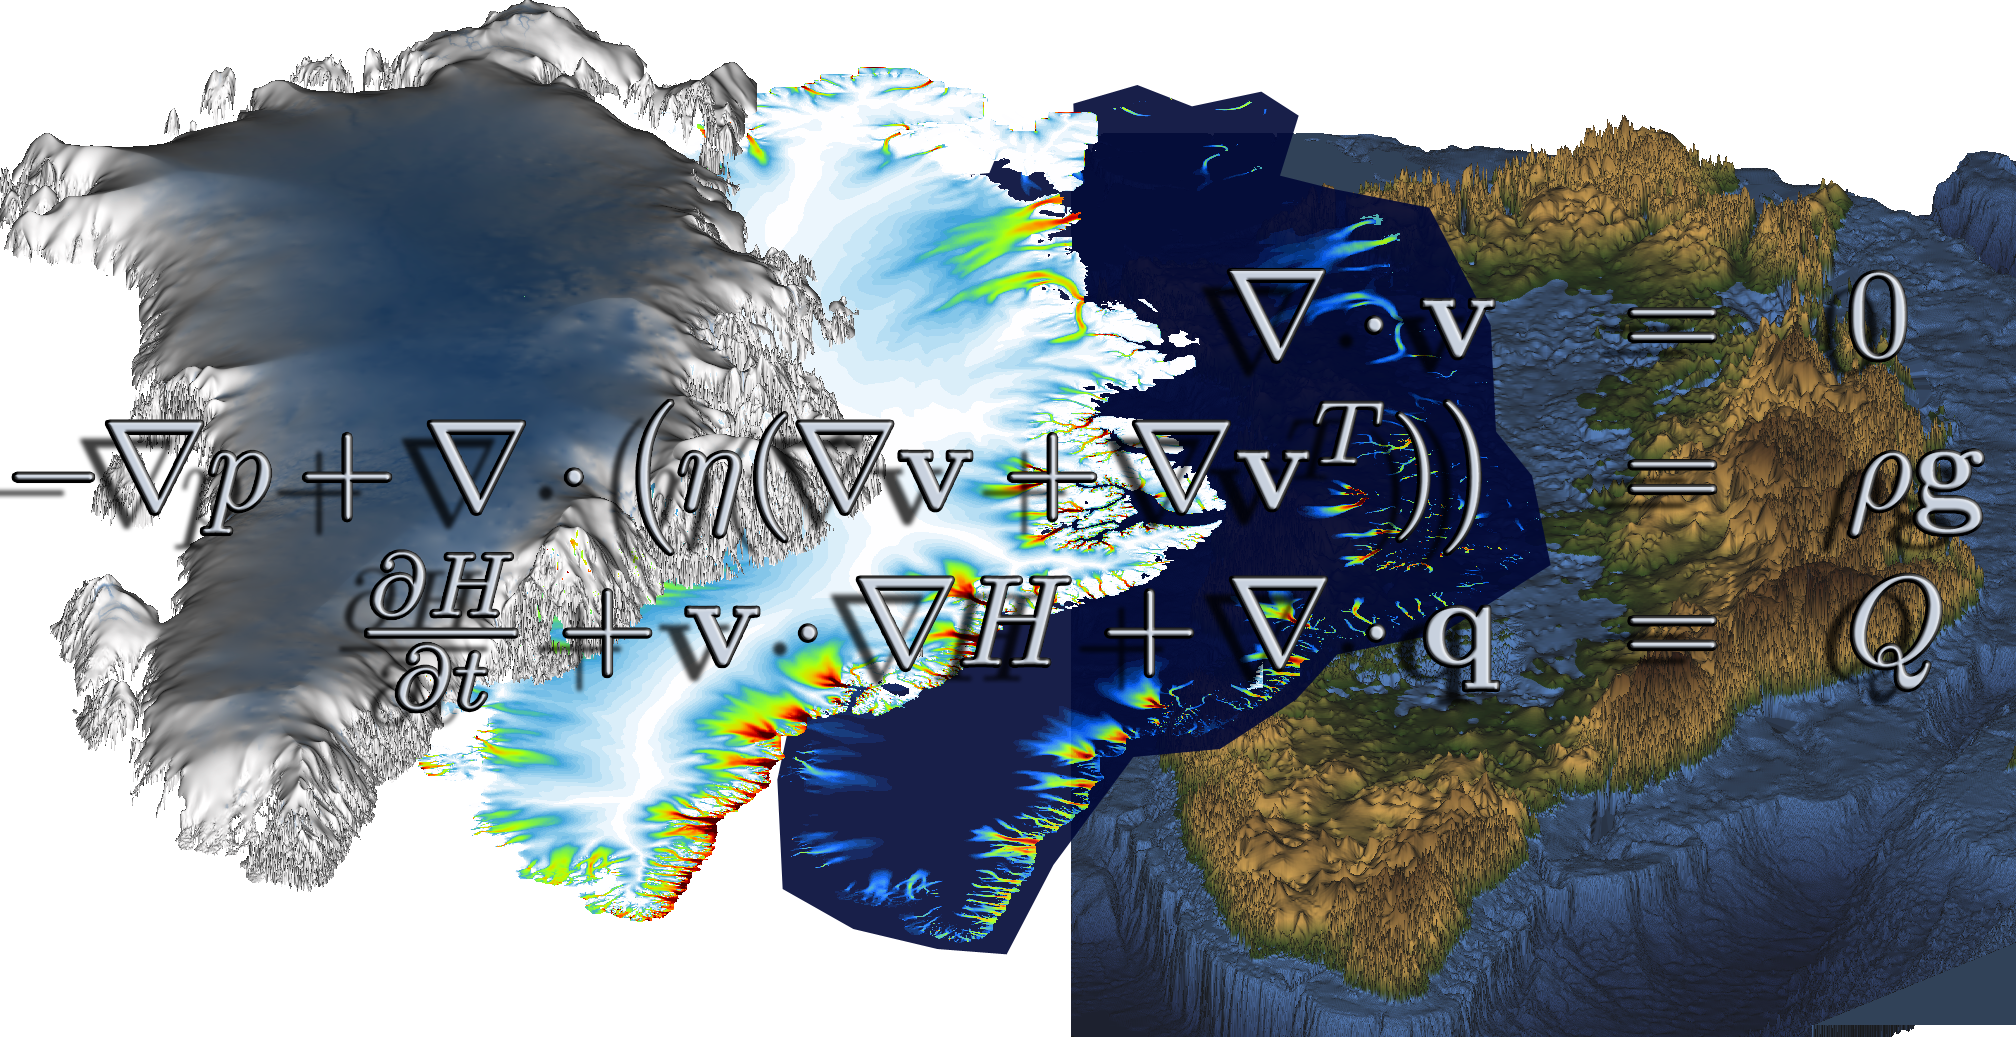
\includegraphics[width=8cm]{grn_system_eqns}
  \end{figure}
  \begin{columns}[c]
    \begin{column}{.40\linewidth}
      \begin{itemize}
      \item ice dynamics
      \item thermodynamics
      \item surface processes
      \end{itemize}
    \end{column}
    \begin{column}{.55\linewidth}
      \begin{itemize}
      \item boundary conditions
      \item hydrology
      \item ice-ocean interaction (e.g. calving)
      \end{itemize}
    \end{column}
  \end{columns}
  \note[item]{An ice sheet model solves numerical approximations to the balance equations of mass, momentum}
  \note[item]{Ice flow is governed by Stokes equations with a power-law rheology}
  \note[item]{Because the viscosity of ice strongly depends on the thermal state, we also need to solve an energy balance equation}
  \note[item]{This makes the problem thermomechanically-coupled.}
\end{frame}


\begin{frame}{Why ice sheet modeling is easy}
  \begin{columns}[c]
    \begin{column}{.28\linewidth}
      \begin{figure}
        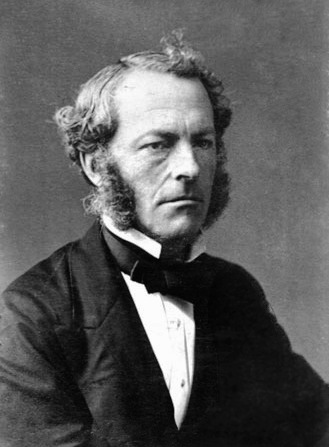
\includegraphics[width=\linewidth]{ggstokes}
        \\ \scriptsize{G.~G.~Stokes}
      \end{figure}
    \end{column}
    \begin{column}{.67\linewidth}
      \begin{itemize}[<+- | alert@+>]
      \item composed of a single, largely homogeneous material
      \item flow governed by the Stokes equations known since the mid-19th century
      \item flows slowly: we can ignore turbulence, Coriolis and other inertial effects
      \item no density/salinity stratification
      \item most of what makes atmosphere and ocean flow interesting is missing
      \item so what makes the flow of slow, cold, laminar ice interesting?
      \end{itemize}
    \end{column}
  \end{columns}
\end{frame}


\begin{frame}{Why ice sheet modeling is so hard}
    \begin{columns}[c]<1-2>
      \begin{column}{.28\linewidth}
        \begin{figure}
          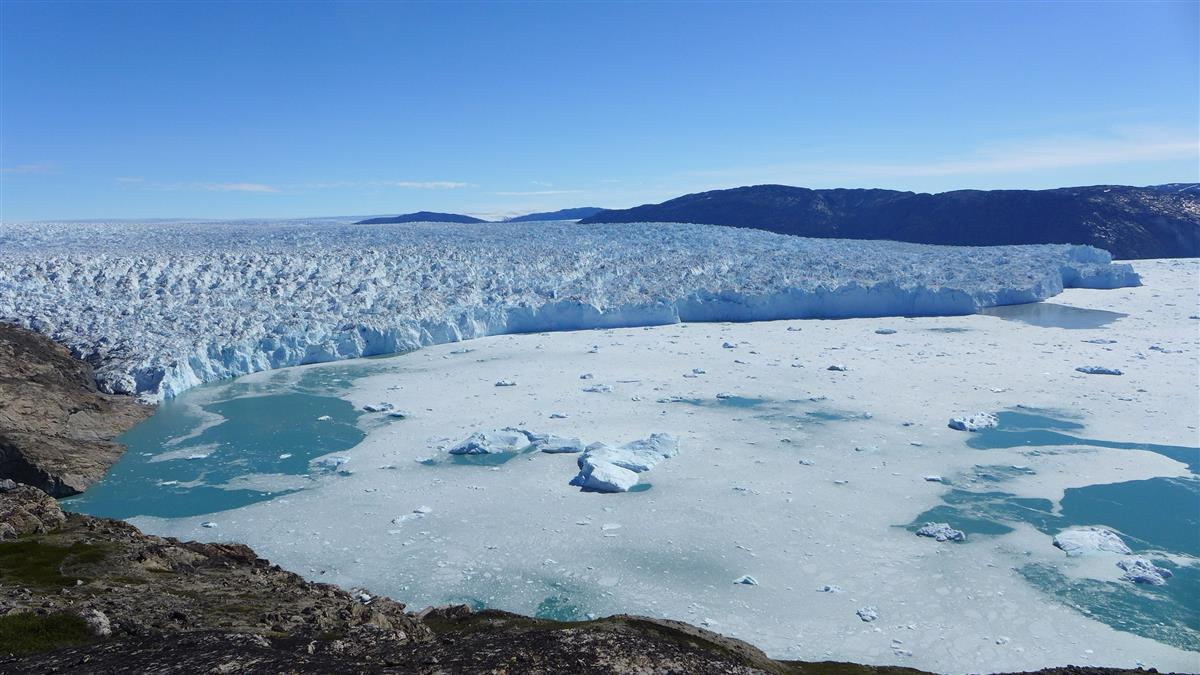
\includegraphics[width=\linewidth]{storeglacier}
        \end{figure}
      \end{column}
      \begin{column}{.67\linewidth}
        \begin{block}{Boundary conditions}
        \begin{itemize}
        \item seaward margin boundary condition
        \item basal boundary condition
        \end{itemize}
      \end{block}
      \end{column}
    \end{columns}
    \begin{columns}[c]<1>
      \begin{column}{.28\linewidth}
        \begin{figure}
          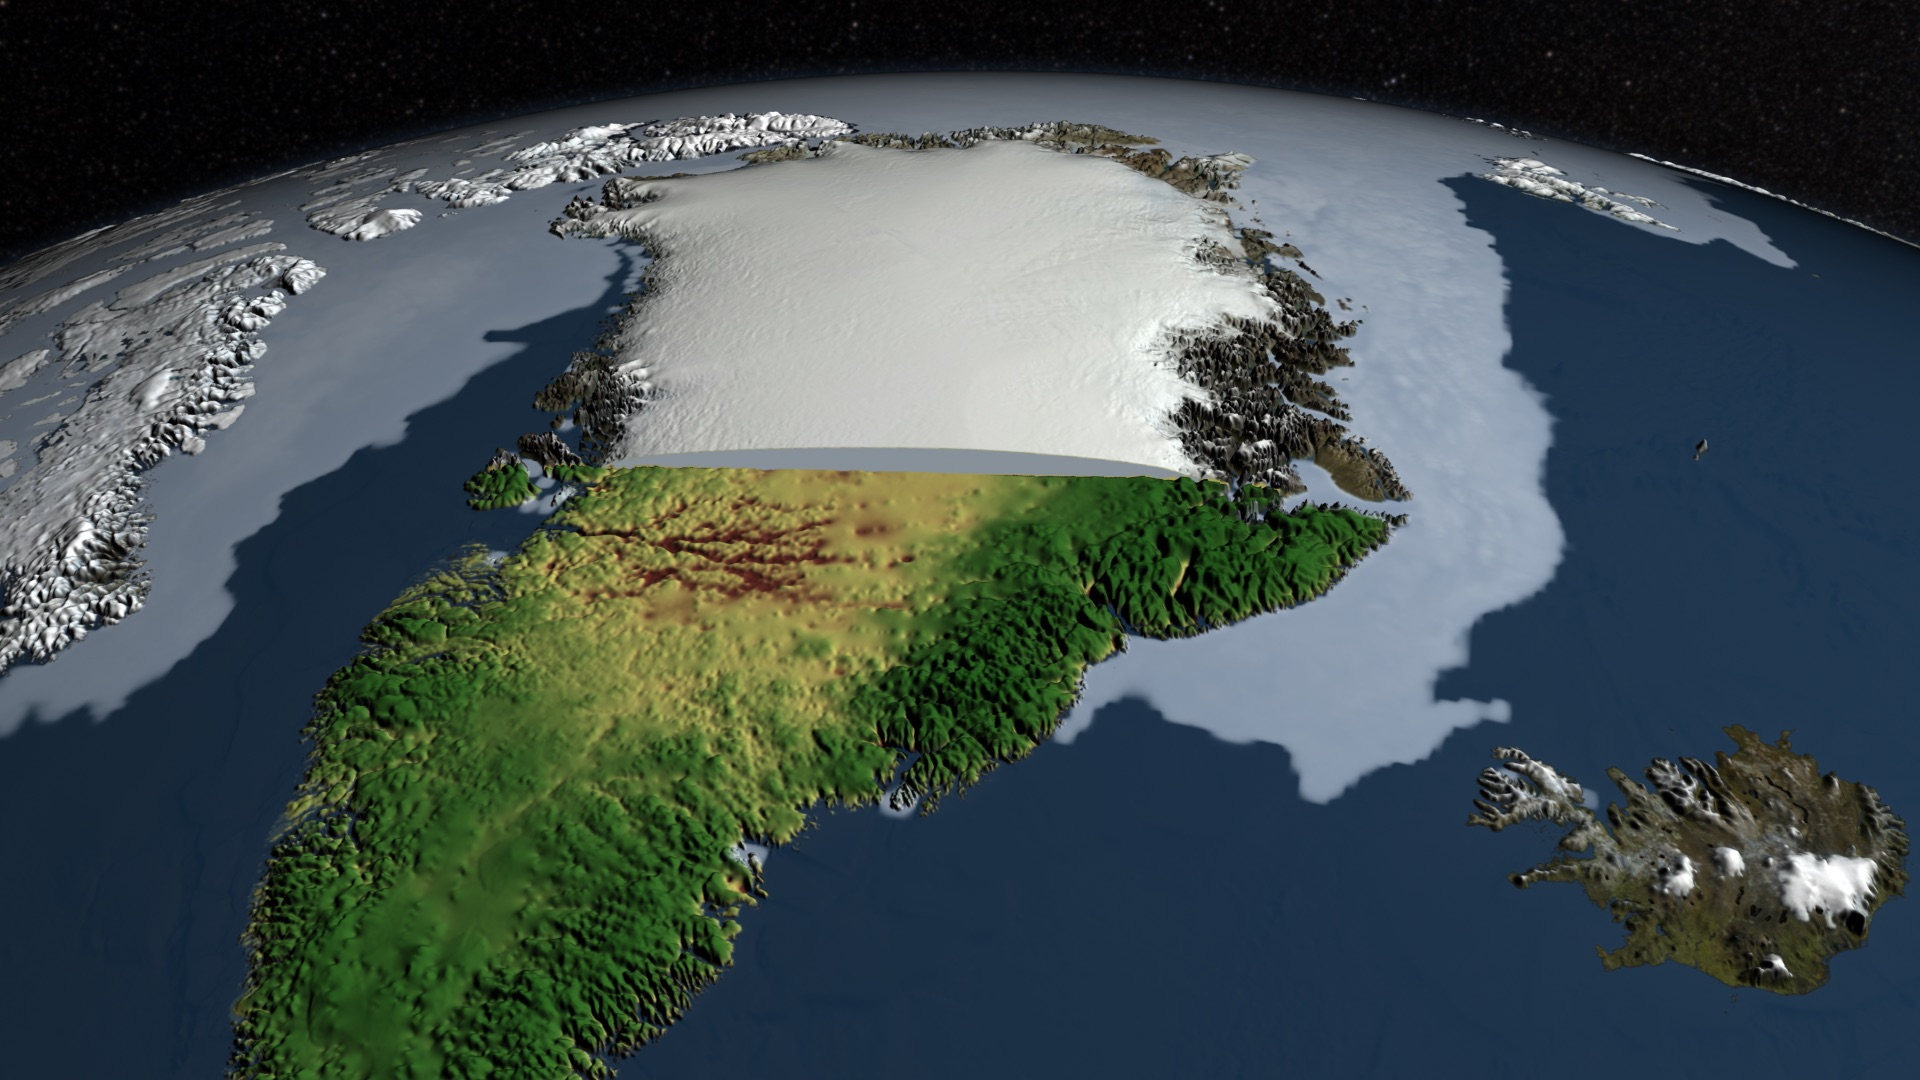
\includegraphics[width=\linewidth]{canale_grande_V05}
        \end{figure}
      \end{column}
      \begin{column}{.67\linewidth}
        \begin{block}{Initial conditions}
        \begin{itemize}
        \item ice thickness / subglacial topography is a first order constraint on ice flow
        \end{itemize}
      \end{block}
      \end{column}
    \end{columns}
    \begin{columns}[c]<1>
      \begin{column}{.3\linewidth}
        \begin{figure}
          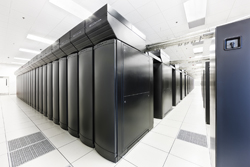
\includegraphics[width=\linewidth]{bw_front_sm}
        \end{figure}
      \end{column}
      \begin{column}{.67\linewidth}
        \begin{block}{Computational costs}
        \begin{itemize}
        \item solving the Stokes equations is computationally very expensive
        \end{itemize}
      \end{block}
      \end{column}
    \end{columns}
\end{frame}


\begin{frame}{Challenge: basal boundary condition}
  \begin{columns}[c]
    \begin{column}{.45\linewidth}
      \begin{figure}
        \scriptsize{basal resistance} \\
        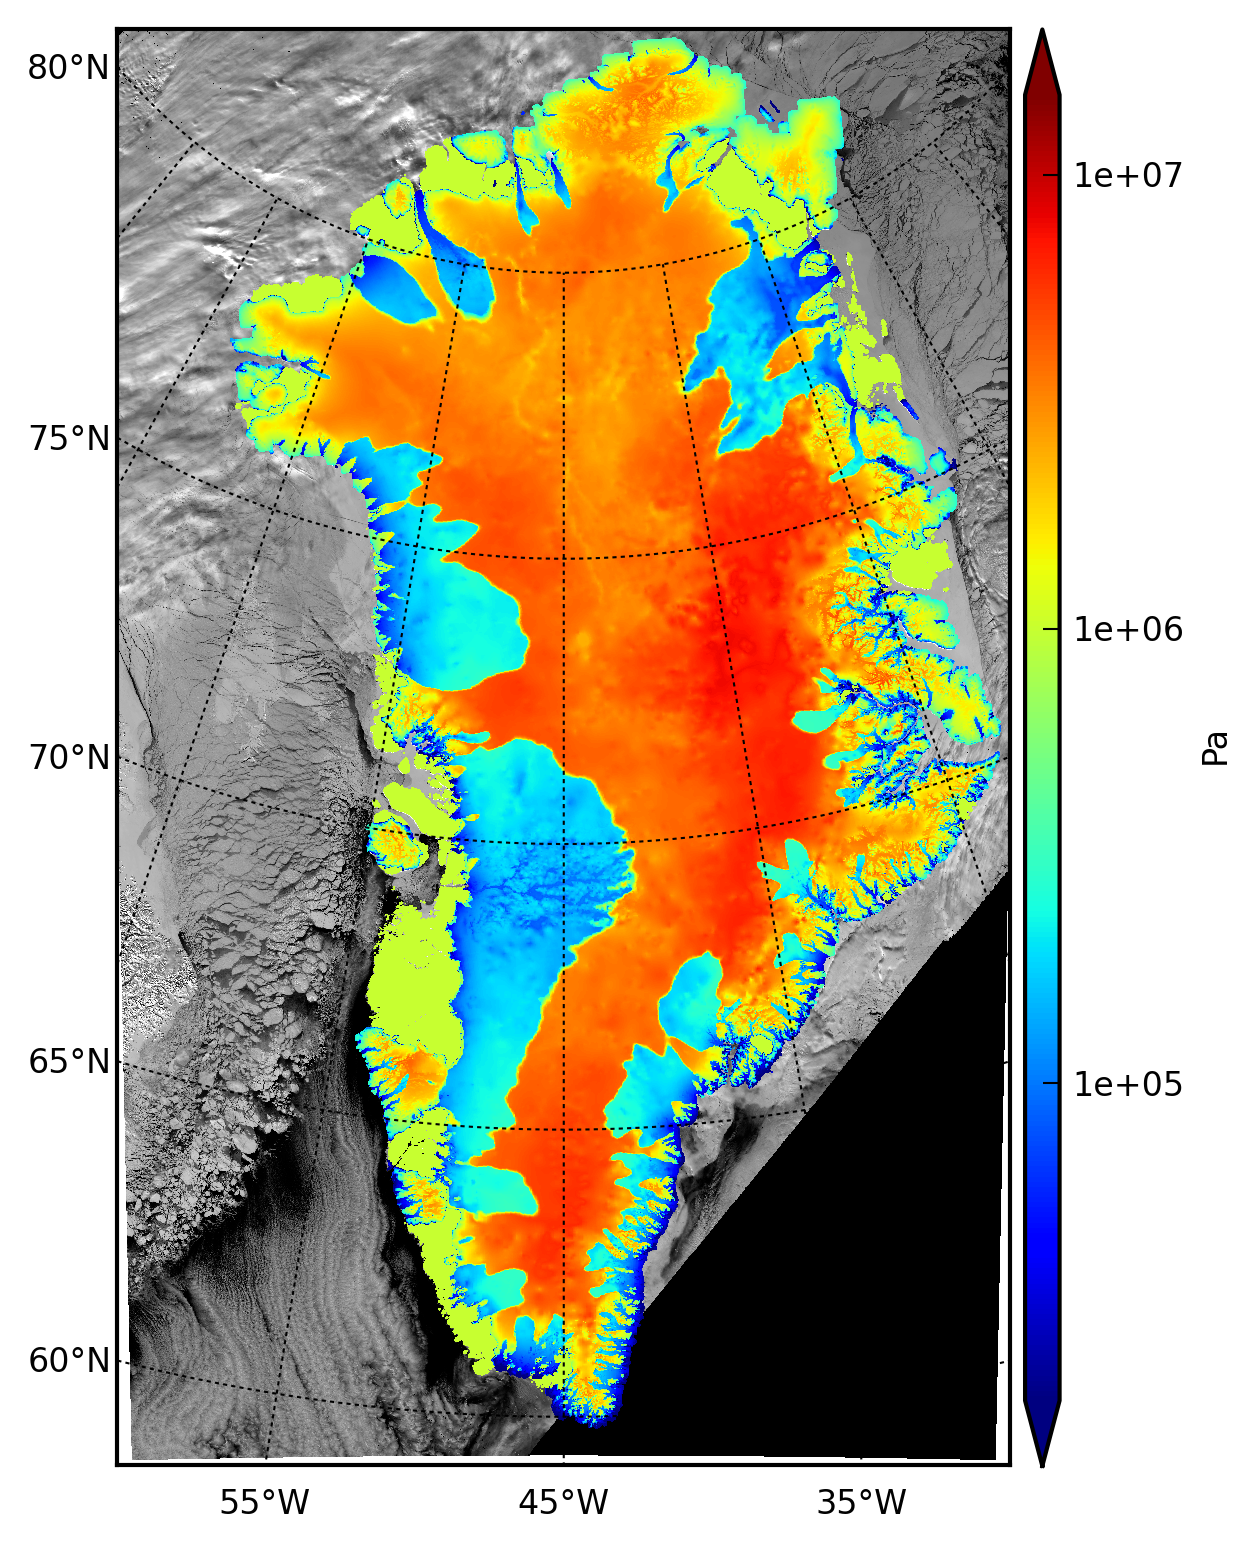
\includegraphics[width=\textwidth]{tauc}
      \end{figure}
    \end{column}
    \begin{column}{.54\linewidth}
      \begin{itemize}
      \item stresses vary by orders of magnitude
      \item basal hydrology, the glacier's ``plumbing system'' runs on a faster ime scale than ice flow
      \item despite more than 5 decades of research, we only have crude parametrizations
      \end{itemize}
    \end{column}
  \end{columns}
  \note[item]{First, stresses at the base vary by several orders of magnitude}
  \note[item]{depend on many factors, most importantly on the presence or absence of water}
  \note[item]{basal hydrology (the glacier's plumbing system) runs on a faster time scale than the ice flow itself}
  \note[item]{but the sub-glacial environment is not easy accessible}
  \note[item]{at the basal boundary, interactions between water flow, friction, heat flow, and sediment deformation is so complex that a deriving a theory from first principles is real challenge}
\end{frame}


\begin{frame}{Challenge: seaward margin boundary condition}
      \begin{figure}
        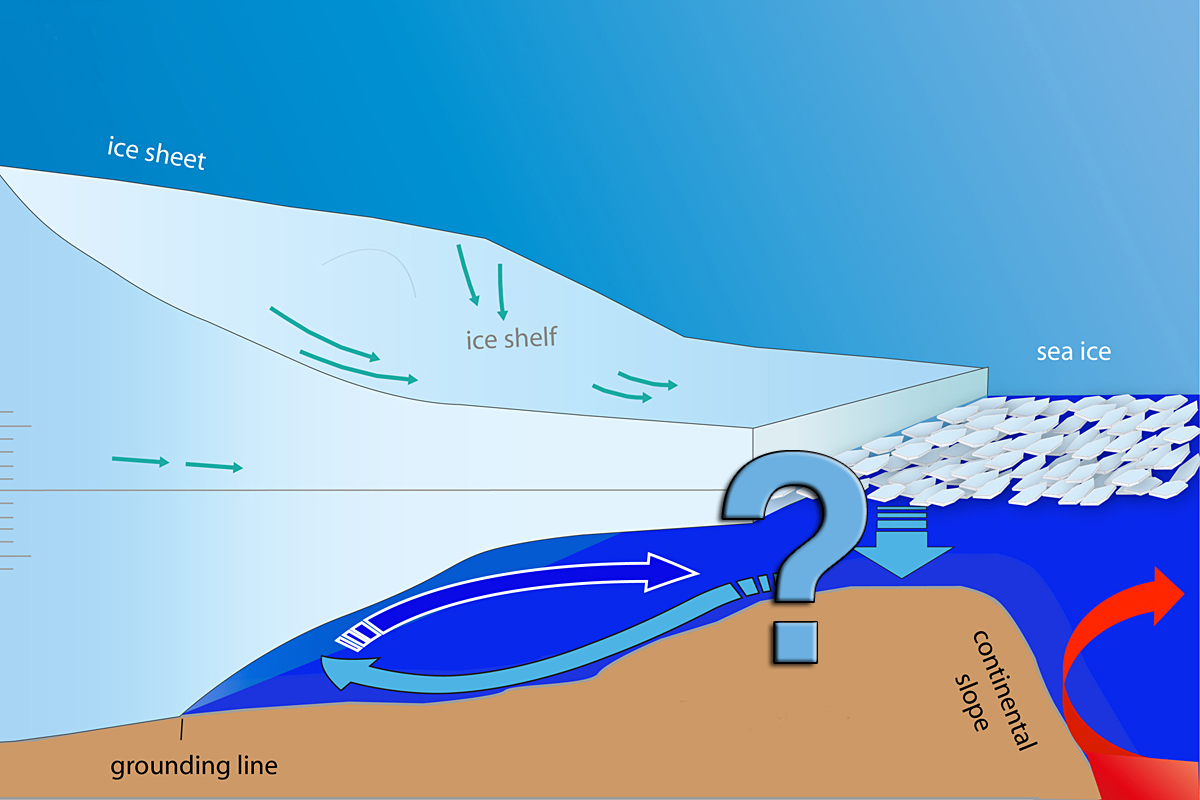
\includegraphics[width=.75\textwidth]{ice-shelf}
      \end{figure}
      \begin{itemize}
      \item ocean circulation $\Rightarrow$ basal melt rates
      \item calving mechanism
      \end{itemize}
      \note[item]{a big challenge is to understand how changing ocean currents and ocean temperatures affects sub-shelf basal melt rates}
      \note[item]{how this can weaken a shelf, and potentially lead to break up}
\end{frame}


\begin{frame}{Why ice sheet modeling is so hard}
    \begin{columns}[c]<1>
      \begin{column}{.28\linewidth}
        \begin{figure}
          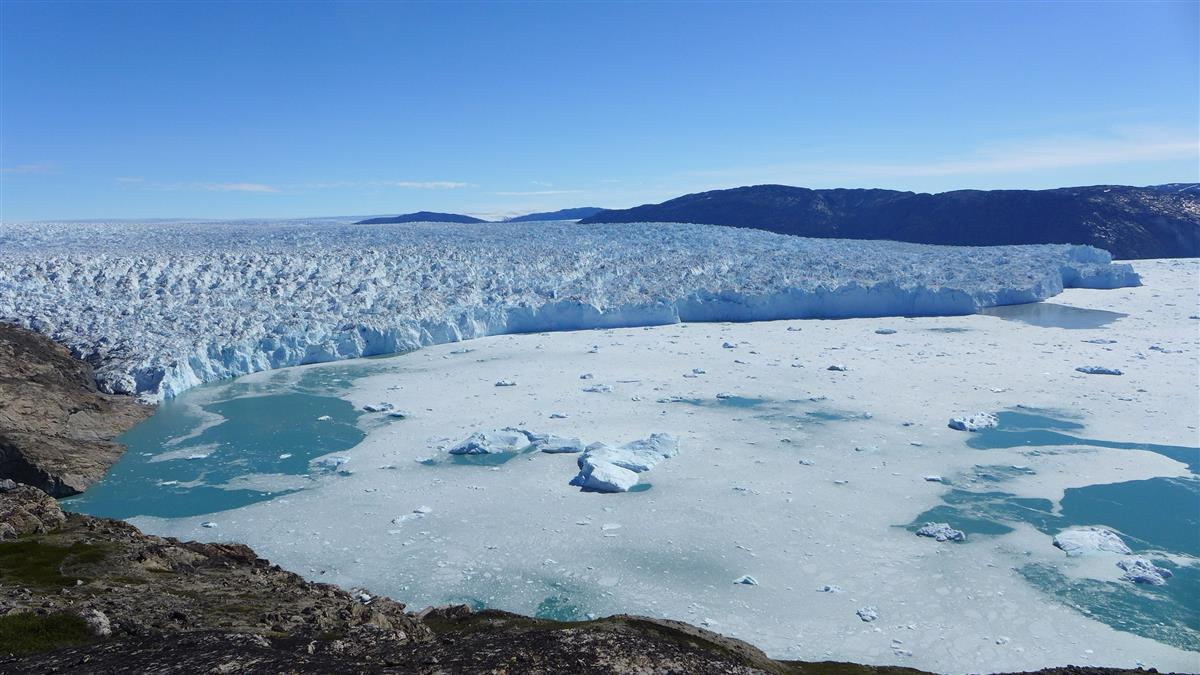
\includegraphics[width=\linewidth]{storeglacier}
        \end{figure}
      \end{column}
      \begin{column}{.67\linewidth}
        \begin{block}{Boundary conditions}
        \begin{itemize}
        \item seaward margin boundary condition
        \item basal boundary condition
        \end{itemize}
      \end{block}
      \end{column}
    \end{columns}
    \begin{columns}[c]<1-2>
      \begin{column}{.28\linewidth}
        \begin{figure}
          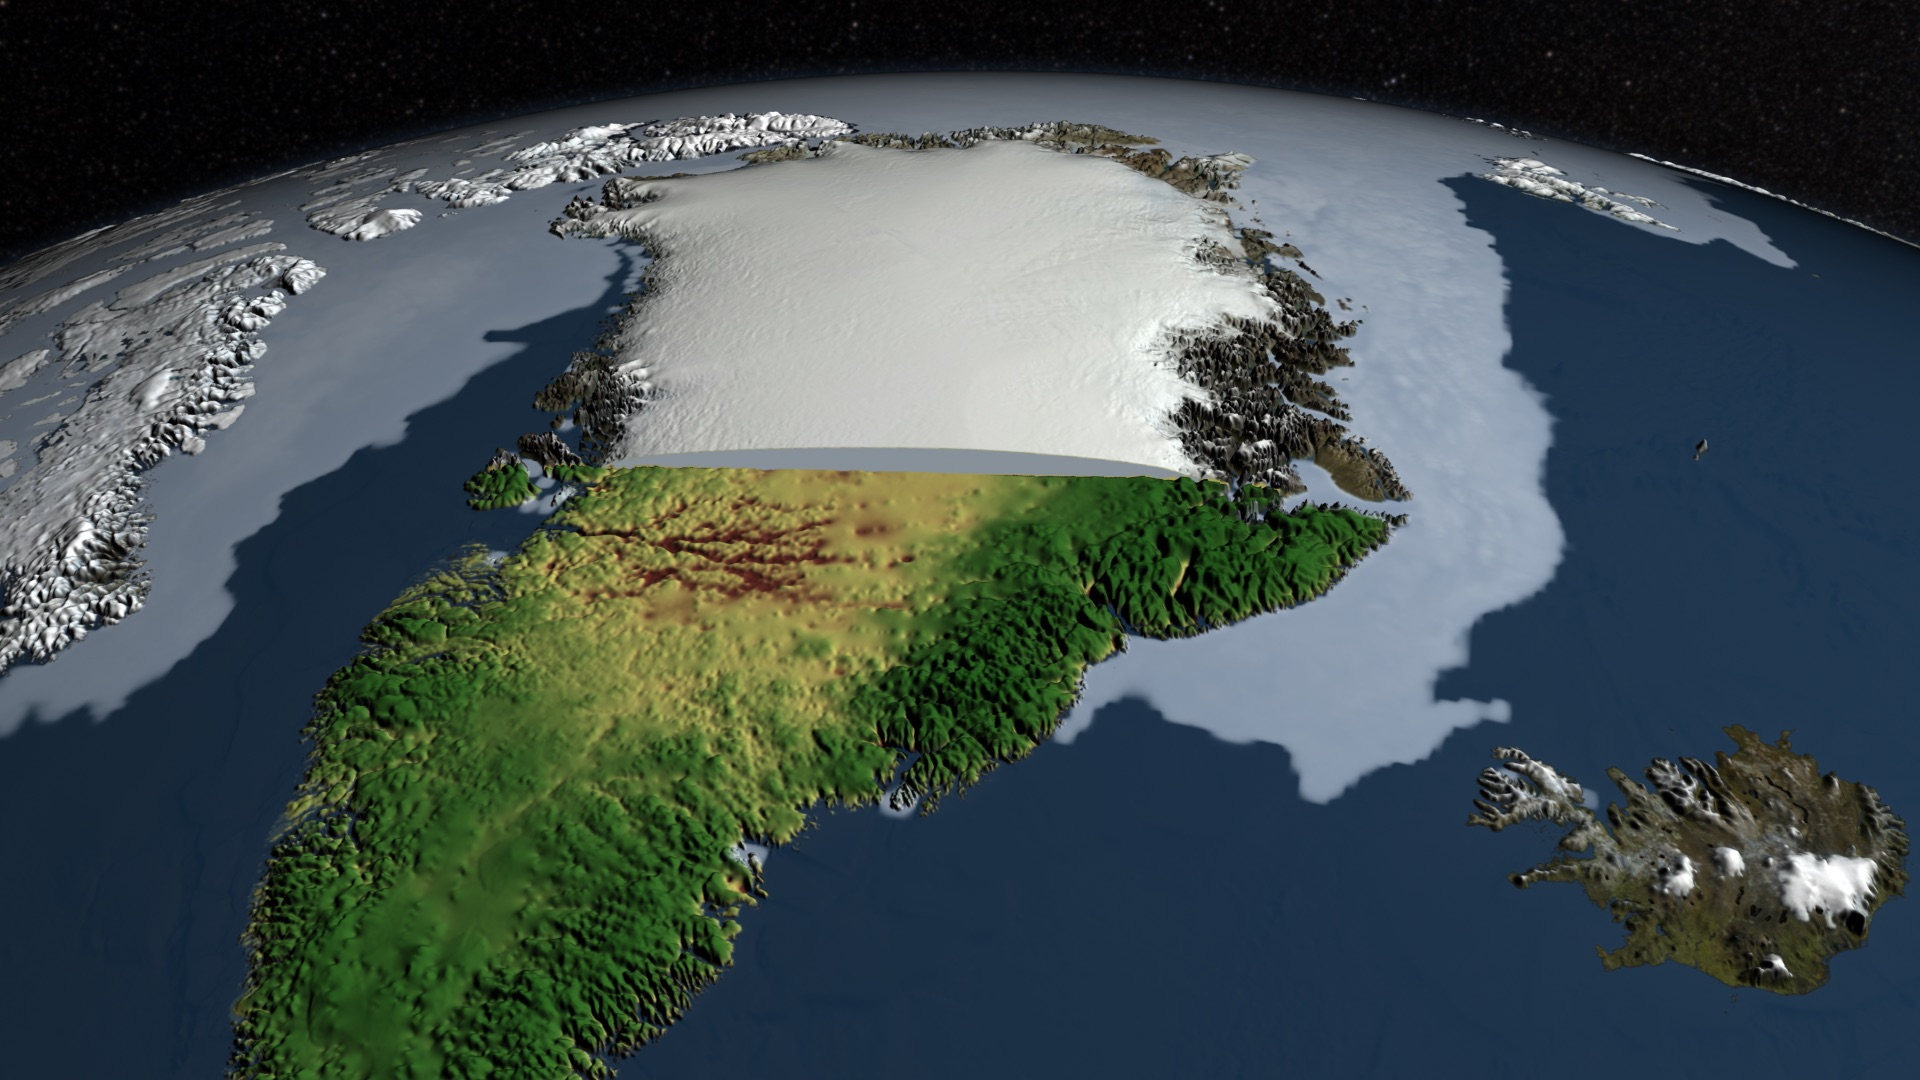
\includegraphics[width=\linewidth]{canale_grande_V05}
        \end{figure}
      \end{column}
      \begin{column}{.67\linewidth}
        \begin{block}{Initial conditions}
        \begin{itemize}
        \item ice thickness / subglacial topography is a first order constraint on ice flow
        \end{itemize}
      \end{block}
      \end{column}
    \end{columns}
    \begin{columns}[c]<1-3>
      \begin{column}{.3\linewidth}
        \begin{figure}
          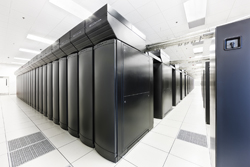
\includegraphics[width=\linewidth]{bw_front_sm}
        \end{figure}
      \end{column}
      \begin{column}{.67\linewidth}
        \begin{block}{Computational costs}
        \begin{itemize}
        \item solving the Stokes equations is computationally very expensive
        \end{itemize}
      \end{block}
      \end{column}
    \end{columns}
    \note<2->[item]{the main focus of my talk is on}
    \note<2->[item]{initial conditions and computational costs}
    \note<2->[item]{solving the Stokes equations is expensive}
\end{frame}


\begin{frame}{1. Simplify the Stokes equations}
  \begin{block}{Ice sheets are shallow}
    \begin{itemize}
    \item below in red is a no-vertical-exaggeration cross section of Greenland at $71^\circ$
      \small
    \item green and blue: standard vertically-exaggerated cross section
    \end{itemize}
    \begin{center}
      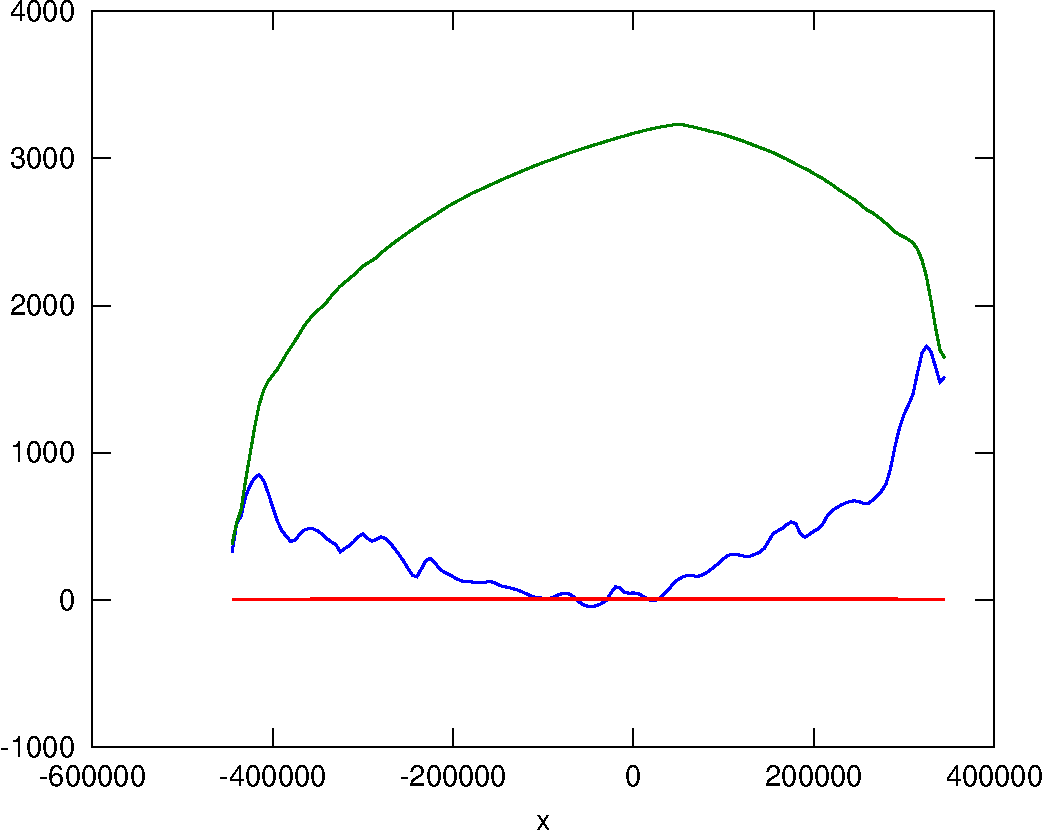
\includegraphics[width=0.4\textwidth]{green_transect} \\
      \footnotesize{Figure by E. Bueler}
    \end{center}
  \end{block}
\end{frame}

\begin{frame}{2. High Performance Computing (HPC)}
  \begin{block}{Exploit modern HPC through parallelism}
    \begin{figure}
      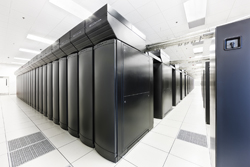
\includegraphics[width=5.5cm]{bw_front_sm}
      \hfill
      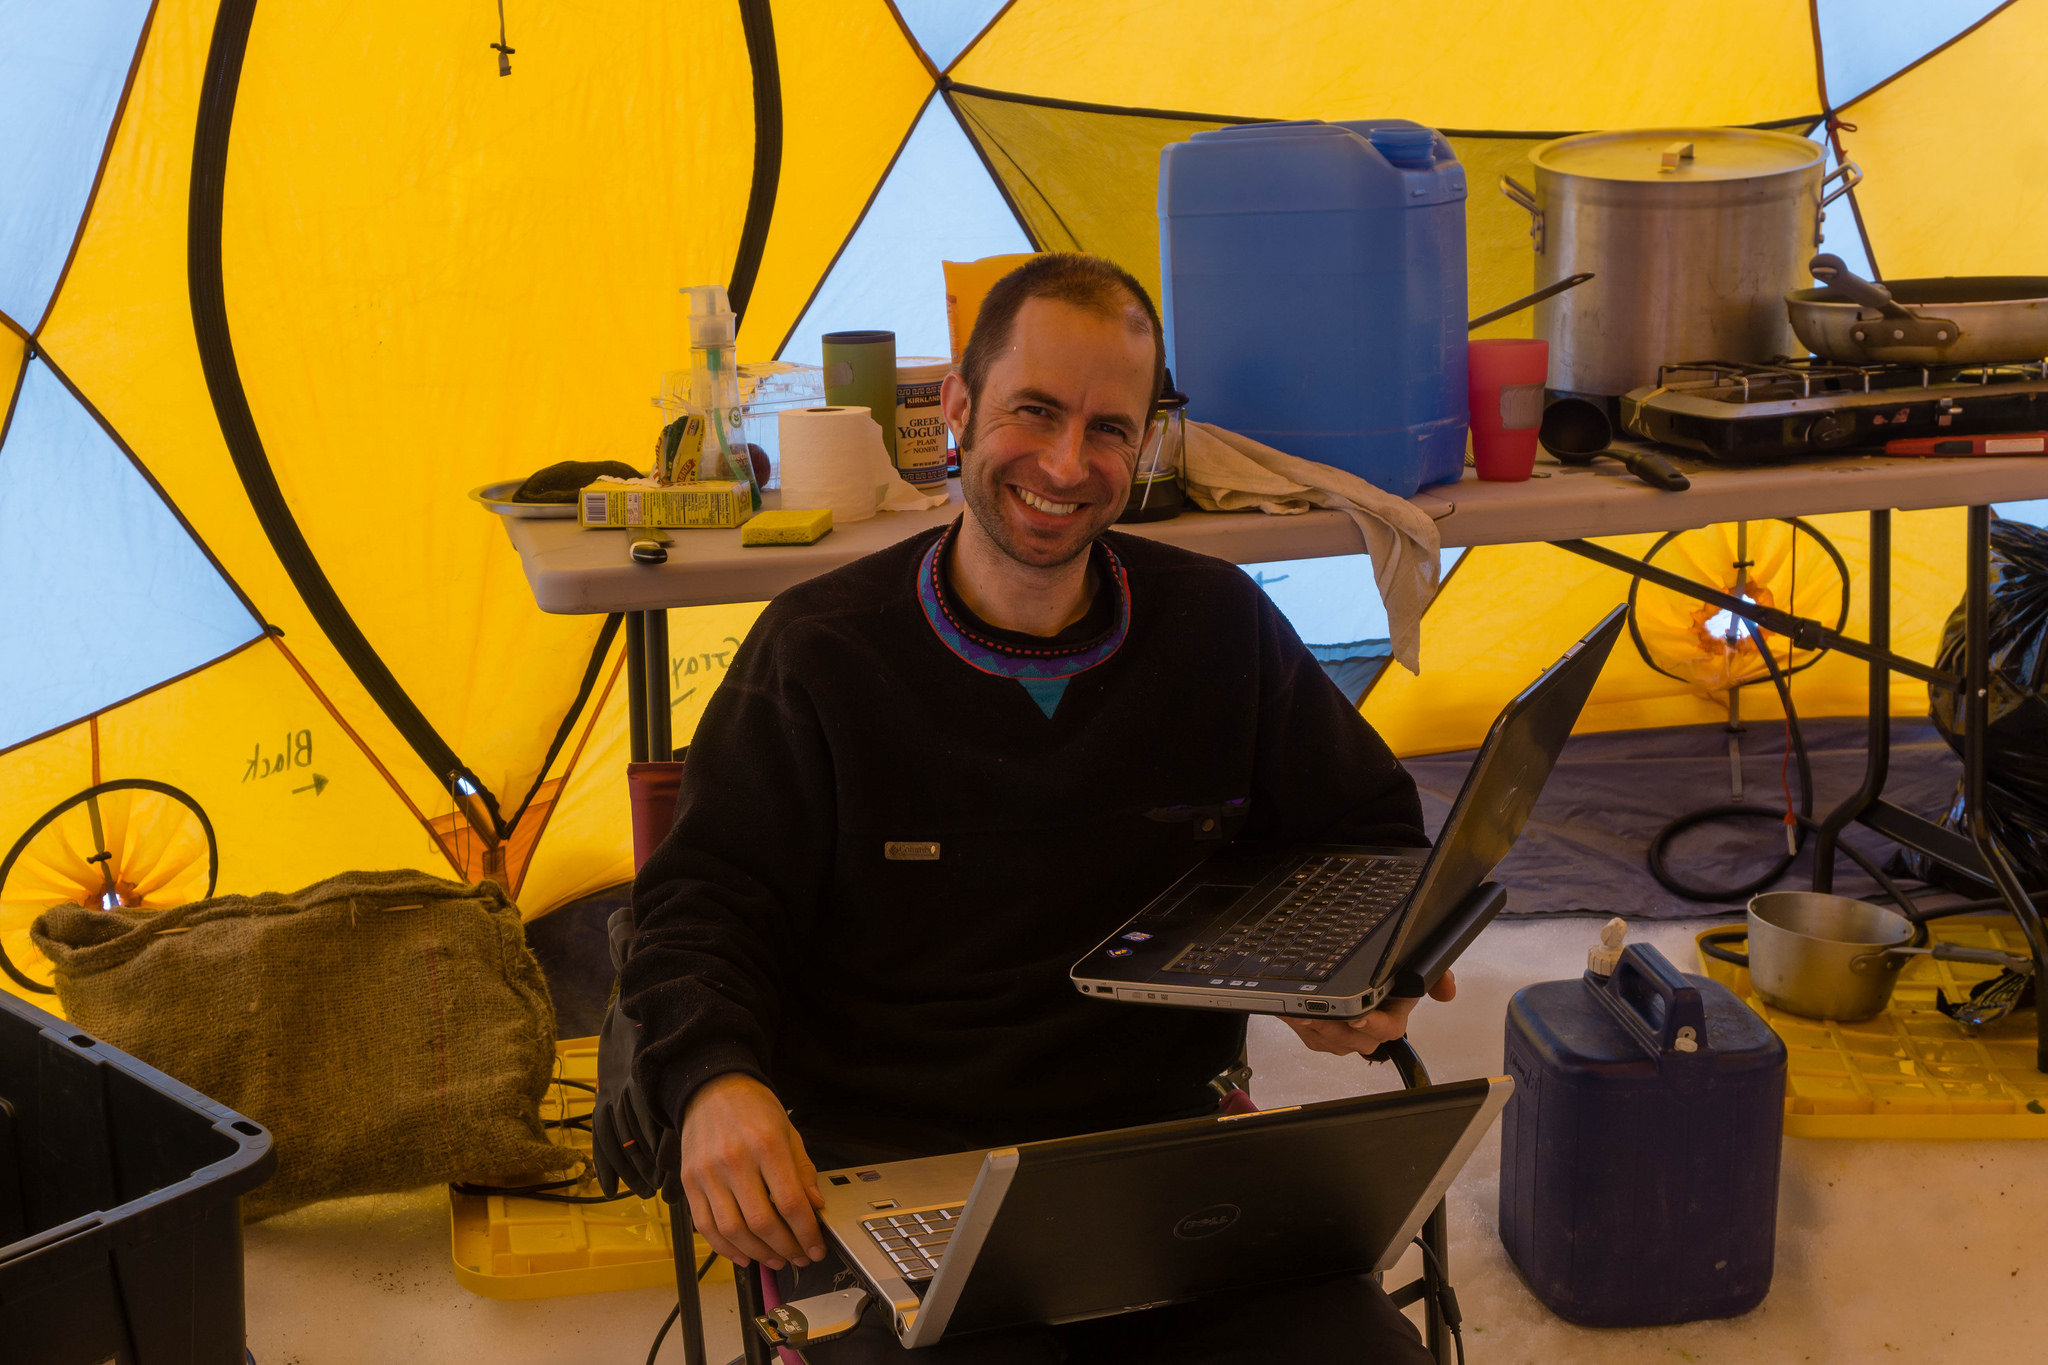
\includegraphics[width=5.5cm]{jason-parallel}
    \end{figure}
  \end{block}
\end{frame}


\begin{frame}{Parallel Ice Sheet Model (PISM)}
  
\includegraphics[width=4cm]{pism-logo}
  \begin{itemize}
  \item open-source, fully-parallel from start in 2006
  \item primary development at UAF, with global user base
  \item $>$100k lines of code; mostly C++
  \item sustained NASA support \tiny (NAG5-11371, NNX09AJ38C, NNX13AM16G, NNX13AK27G), PI's Bueler, Aschwanden
  \end{itemize}
  \begin{columns}
    \column[c]{4.75cm}
    \begin{figure}
      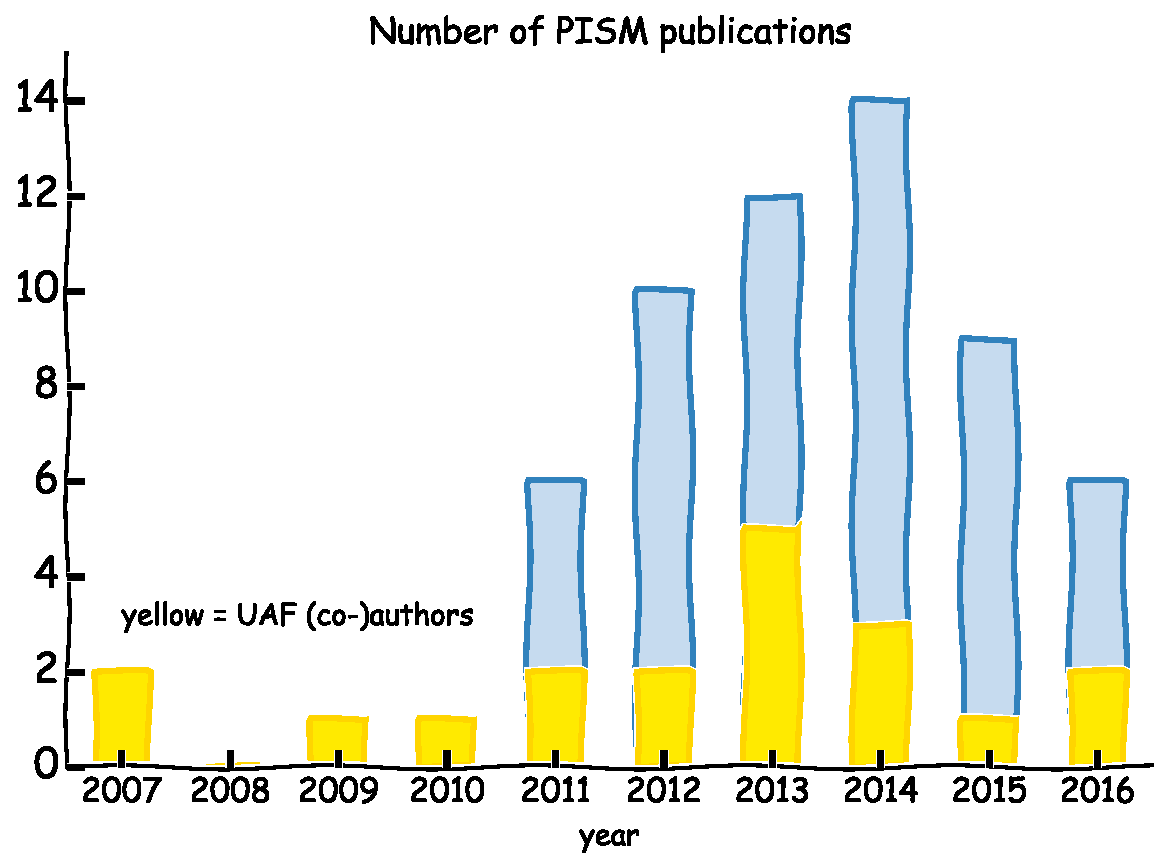
\includegraphics[width=\textwidth]{pism-uaf-publications}
    \end{figure}
    \column[c]{6.25cm}
    \includegraphics<1>[width=\textwidth]{pism-users}
  \end{columns}
\end{frame}

\begin{frame}{Parallel Ice Sheet Model (PISM) cont.}
  
\includegraphics[width=4cm]{pism-logo}
  \begin{itemize}
  \item PISM uses a computationally-efficient approximation to the Stokes equations
  \item PISM runs on large HPC systems
  \item currently installed on GI RCS's pacman, fish, \& chinook, as well as on NASA's pleiades cluster
  \item simulations typically use 100-500 cores and may take up to two weeks wall time to complete
  \end{itemize}
\end{frame}


\begin{frame}{Why ice sheet modeling is so hard}
    \begin{columns}[c]<1>
      \begin{column}{.28\linewidth}
        \begin{figure}
          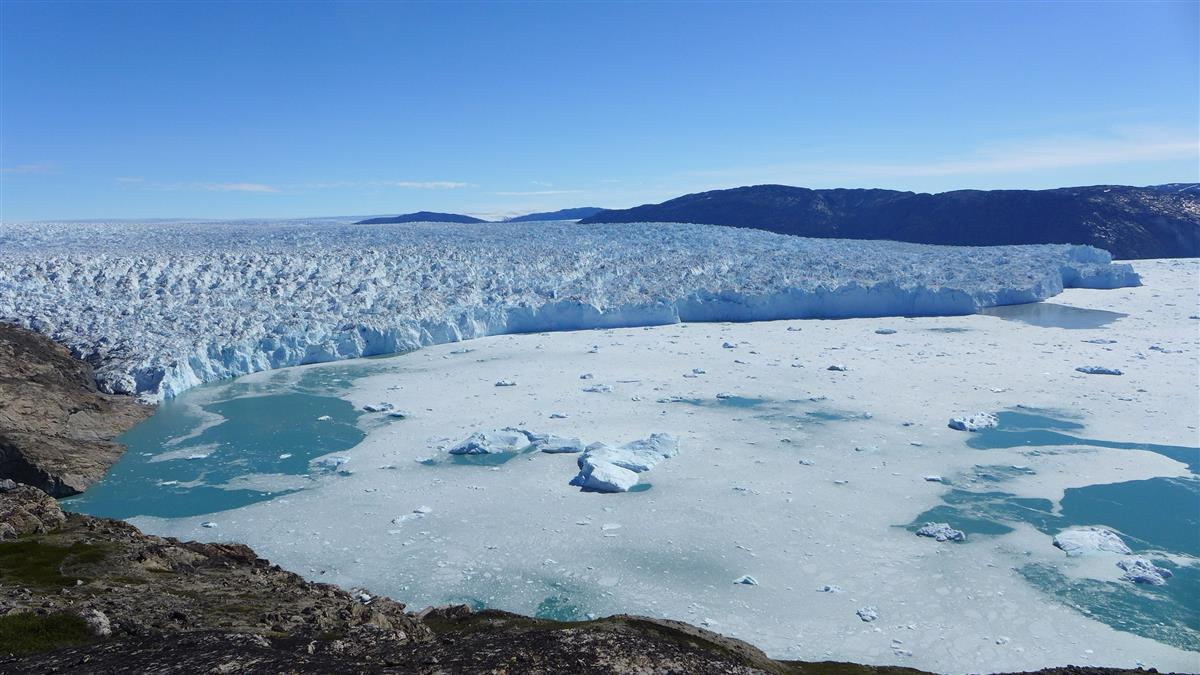
\includegraphics[width=\linewidth]{storeglacier}
        \end{figure}
      \end{column}
      \begin{column}{.67\linewidth}
        \begin{block}{Boundary conditions}
        \begin{itemize}
        \item seaward margin boundary condition
        \item basal boundary condition
        \end{itemize}
      \end{block}
      \end{column}
    \end{columns}
    \begin{columns}[c]<1-2>
      \begin{column}{.28\linewidth}
        \begin{figure}
          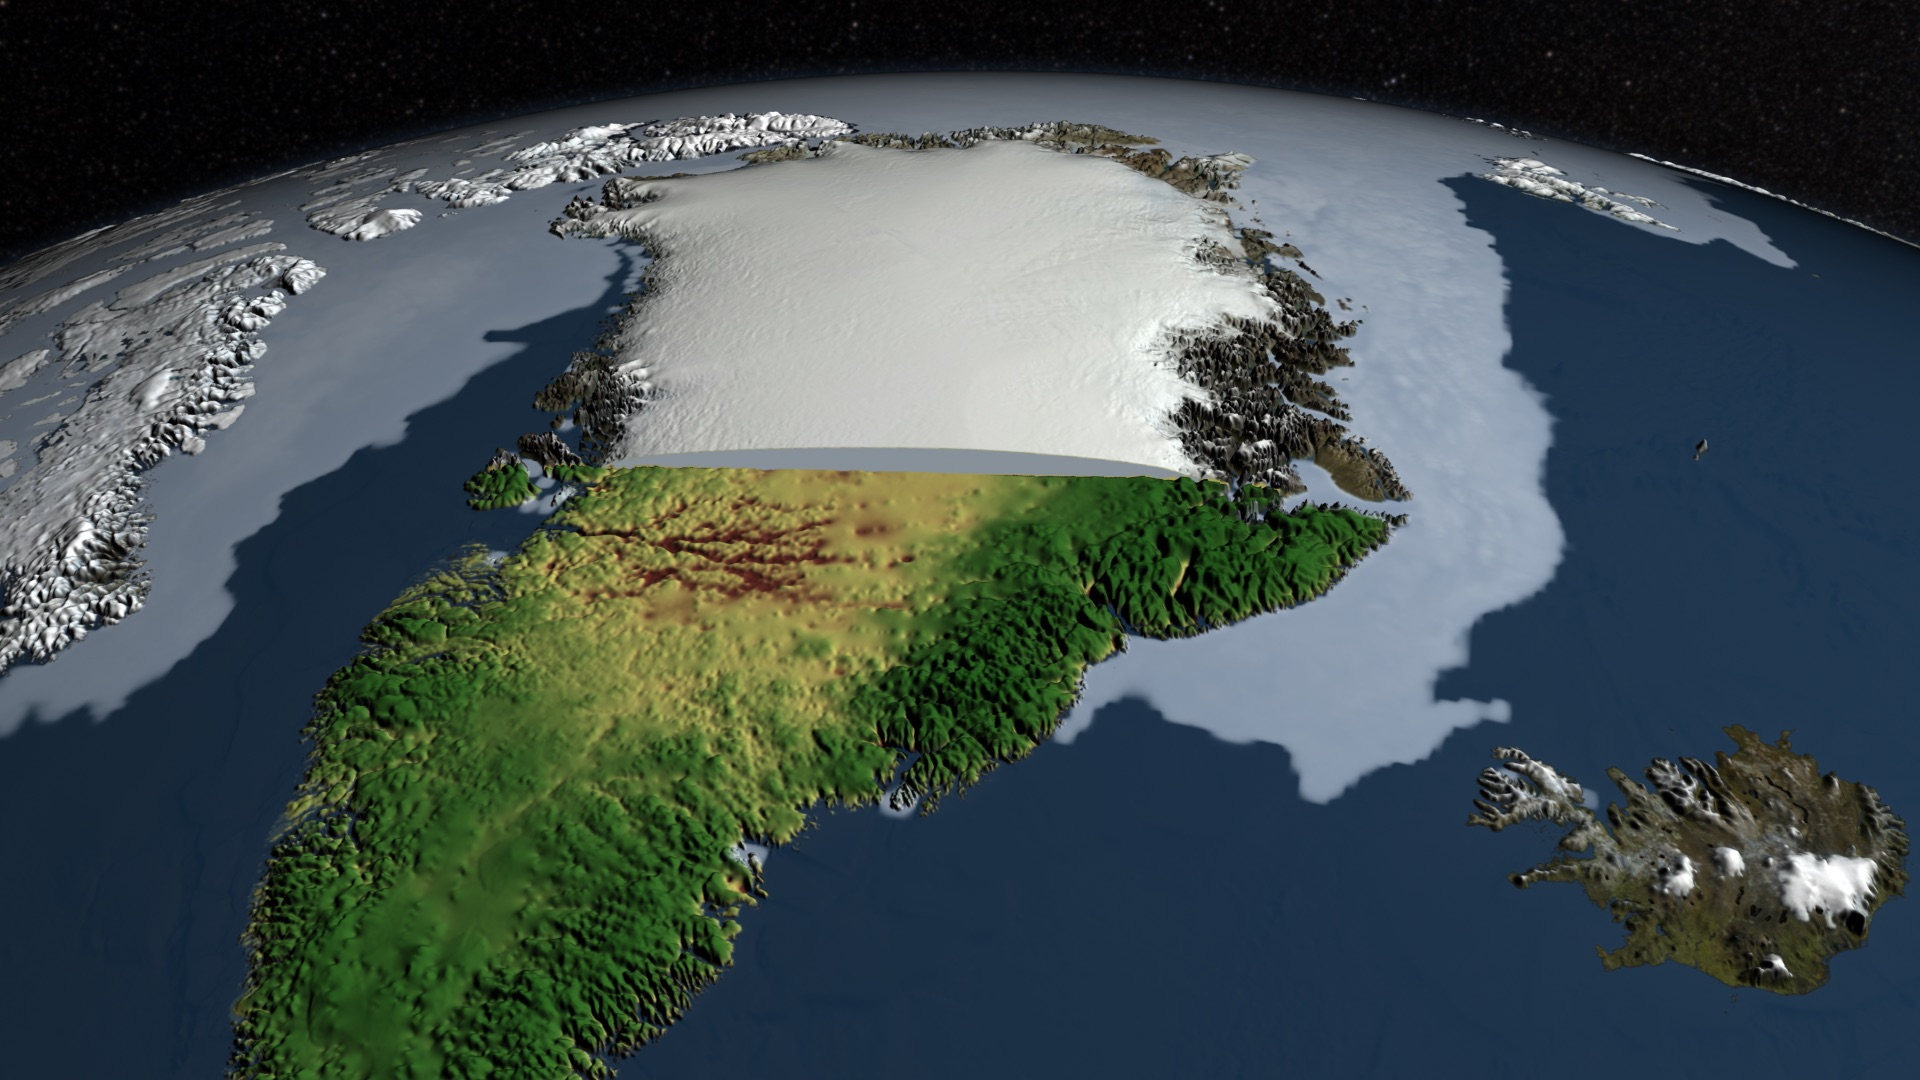
\includegraphics[width=\linewidth]{canale_grande_V05}
        \end{figure}
      \end{column}
      \begin{column}{.67\linewidth}
        \begin{block}{Initial conditions}
        \begin{itemize}
        \item ice thickness / subglacial topography is a first order constraint on ice flow
        \end{itemize}
      \end{block}
      \end{column}
    \end{columns}
    \begin{columns}[c]<1>
      \begin{column}{.3\linewidth}
        \begin{figure}
          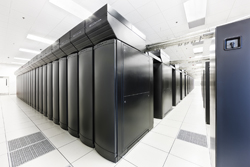
\includegraphics[width=\linewidth]{bw_front_sm}
        \end{figure}
      \end{column}
      \begin{column}{.67\linewidth}
        \begin{block}{Computational costs}
        \begin{itemize}
        \item solving the Stokes equations is computationally very expensive
        \end{itemize}
      \end{block}
      \end{column}
    \end{columns}
\end{frame}


\begin{frame}{Challenge: ice thickness}
  \begin{columns}
    \column[c]{1.25cm}
    
\includegraphics[width=\textwidth]{nasa-logo} \\
    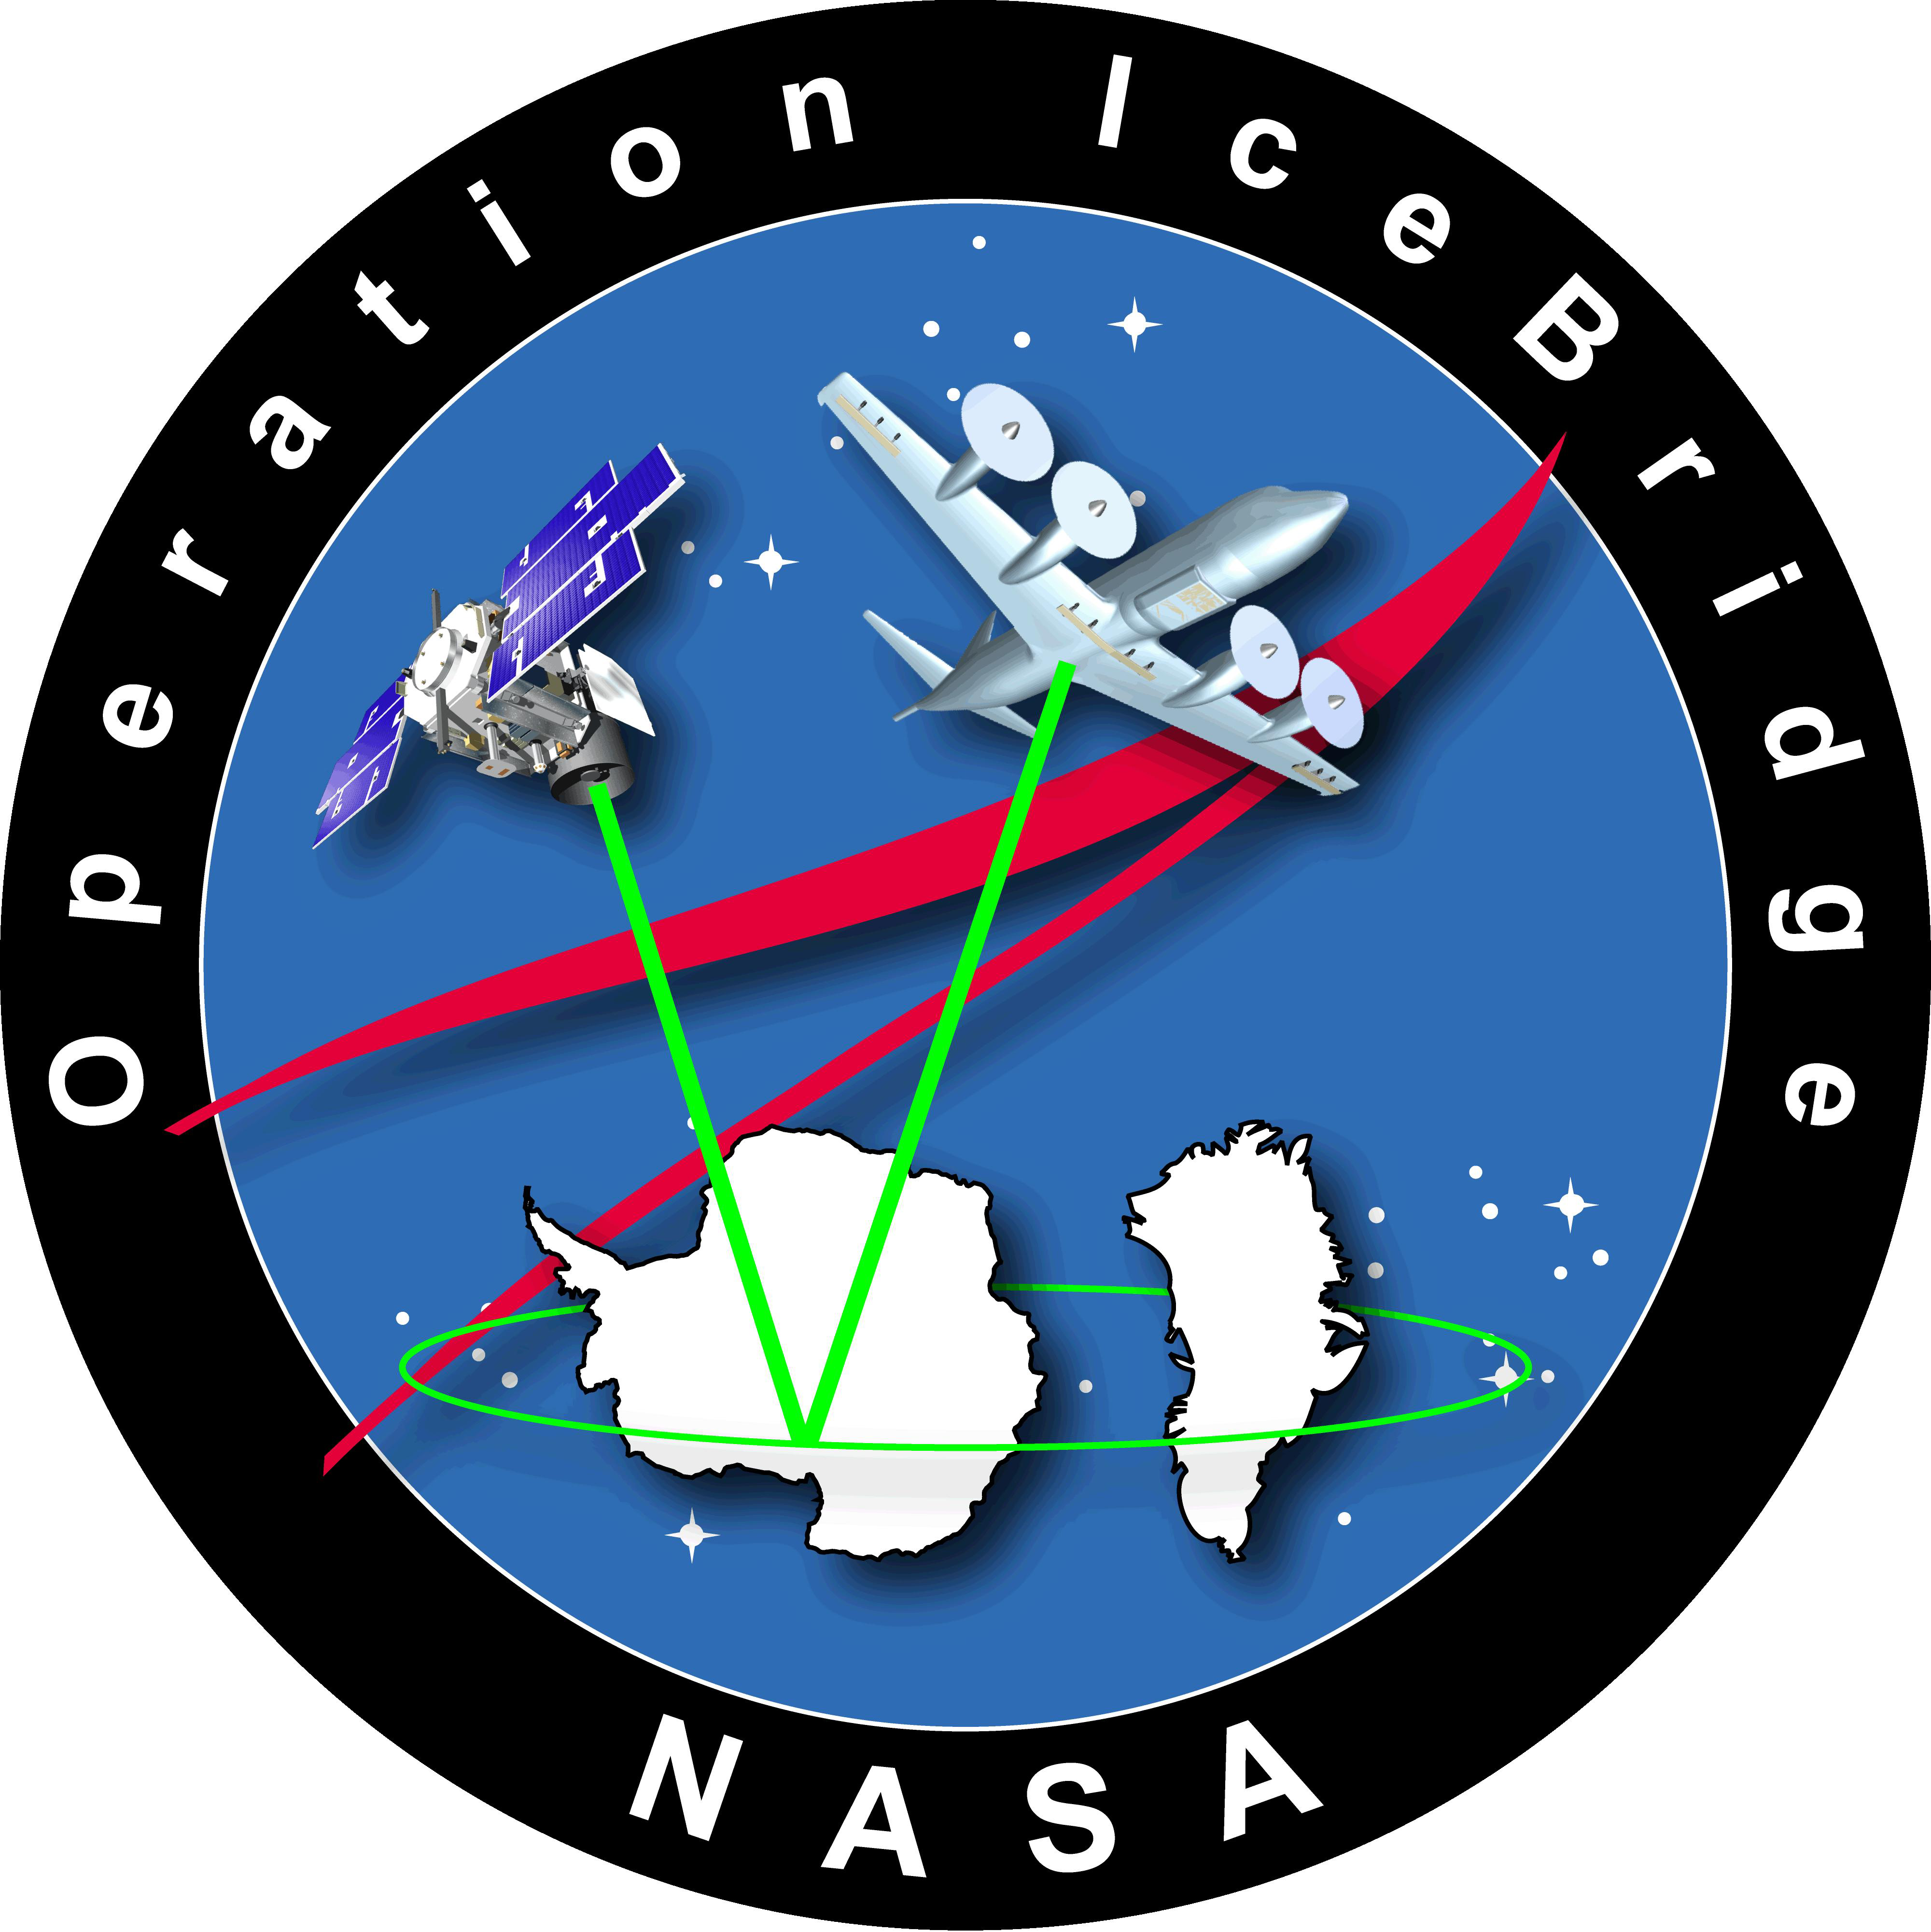
\includegraphics[width=\textwidth]{oib}
    \column[c]{10cm}
    \begin{itemize}
    \item ice thickness is a leading order constraint on ice flow
    \item but expensive to measure
    \item NASA realized that collecting a lot more ice thickness measurements is crucial to make ice sheet models better
    \item ice thickness measurements using the CReSIS radar became an important part of their Operation IceBridge mission (2009--today)
    \end{itemize}
  \end{columns}
  \begin{figure}
    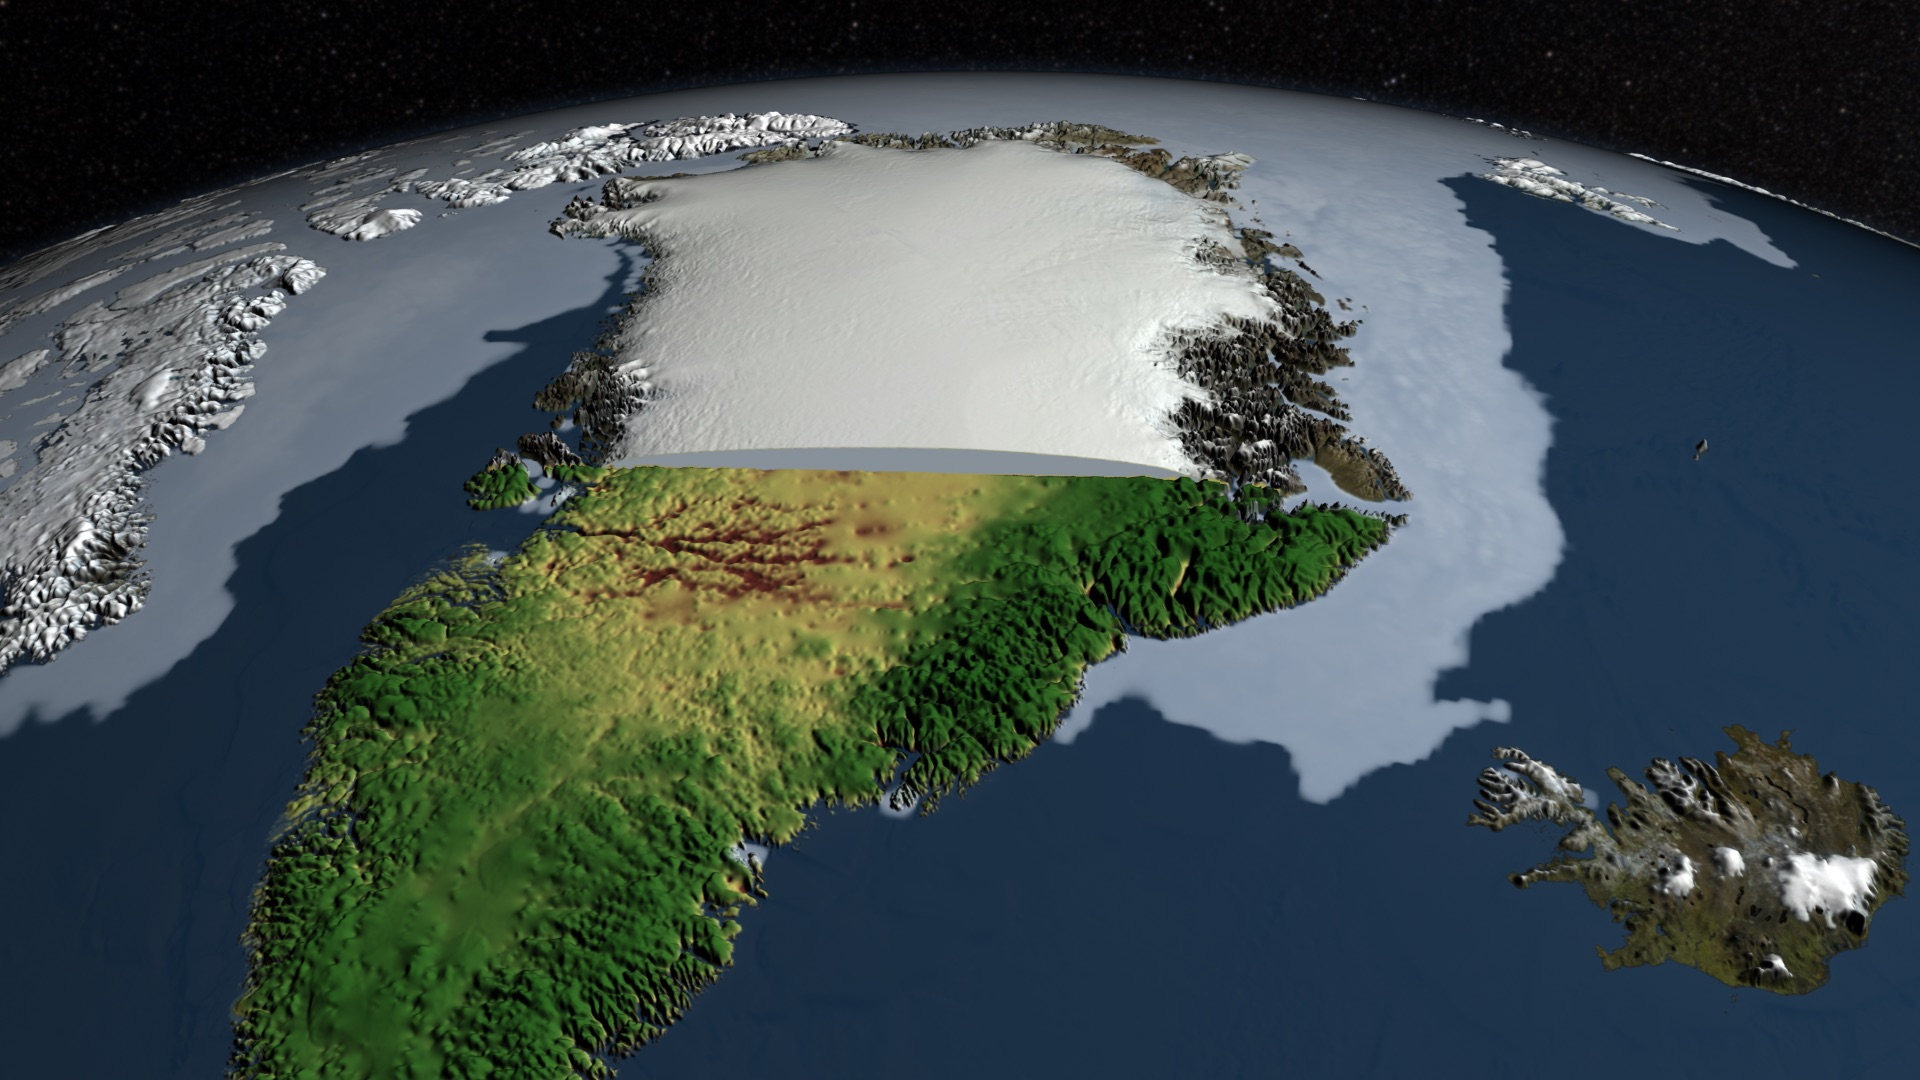
\includegraphics[width=6cm]{canale_grande_V05}
  \end{figure}
\note[item]{ice thickness is the difference between ice upper surface and the subglacial topography}
\end{frame}


\begin{frame}{NASA Operation IceBridge}
  \vspace{-0.74em}
  \begin{columns}
    \column[c]{4cm}
    \begin{itemize}
    \item additional flight lines since 2009
    \end{itemize}
    \column[c]{6cm}
    \begin{figure}
      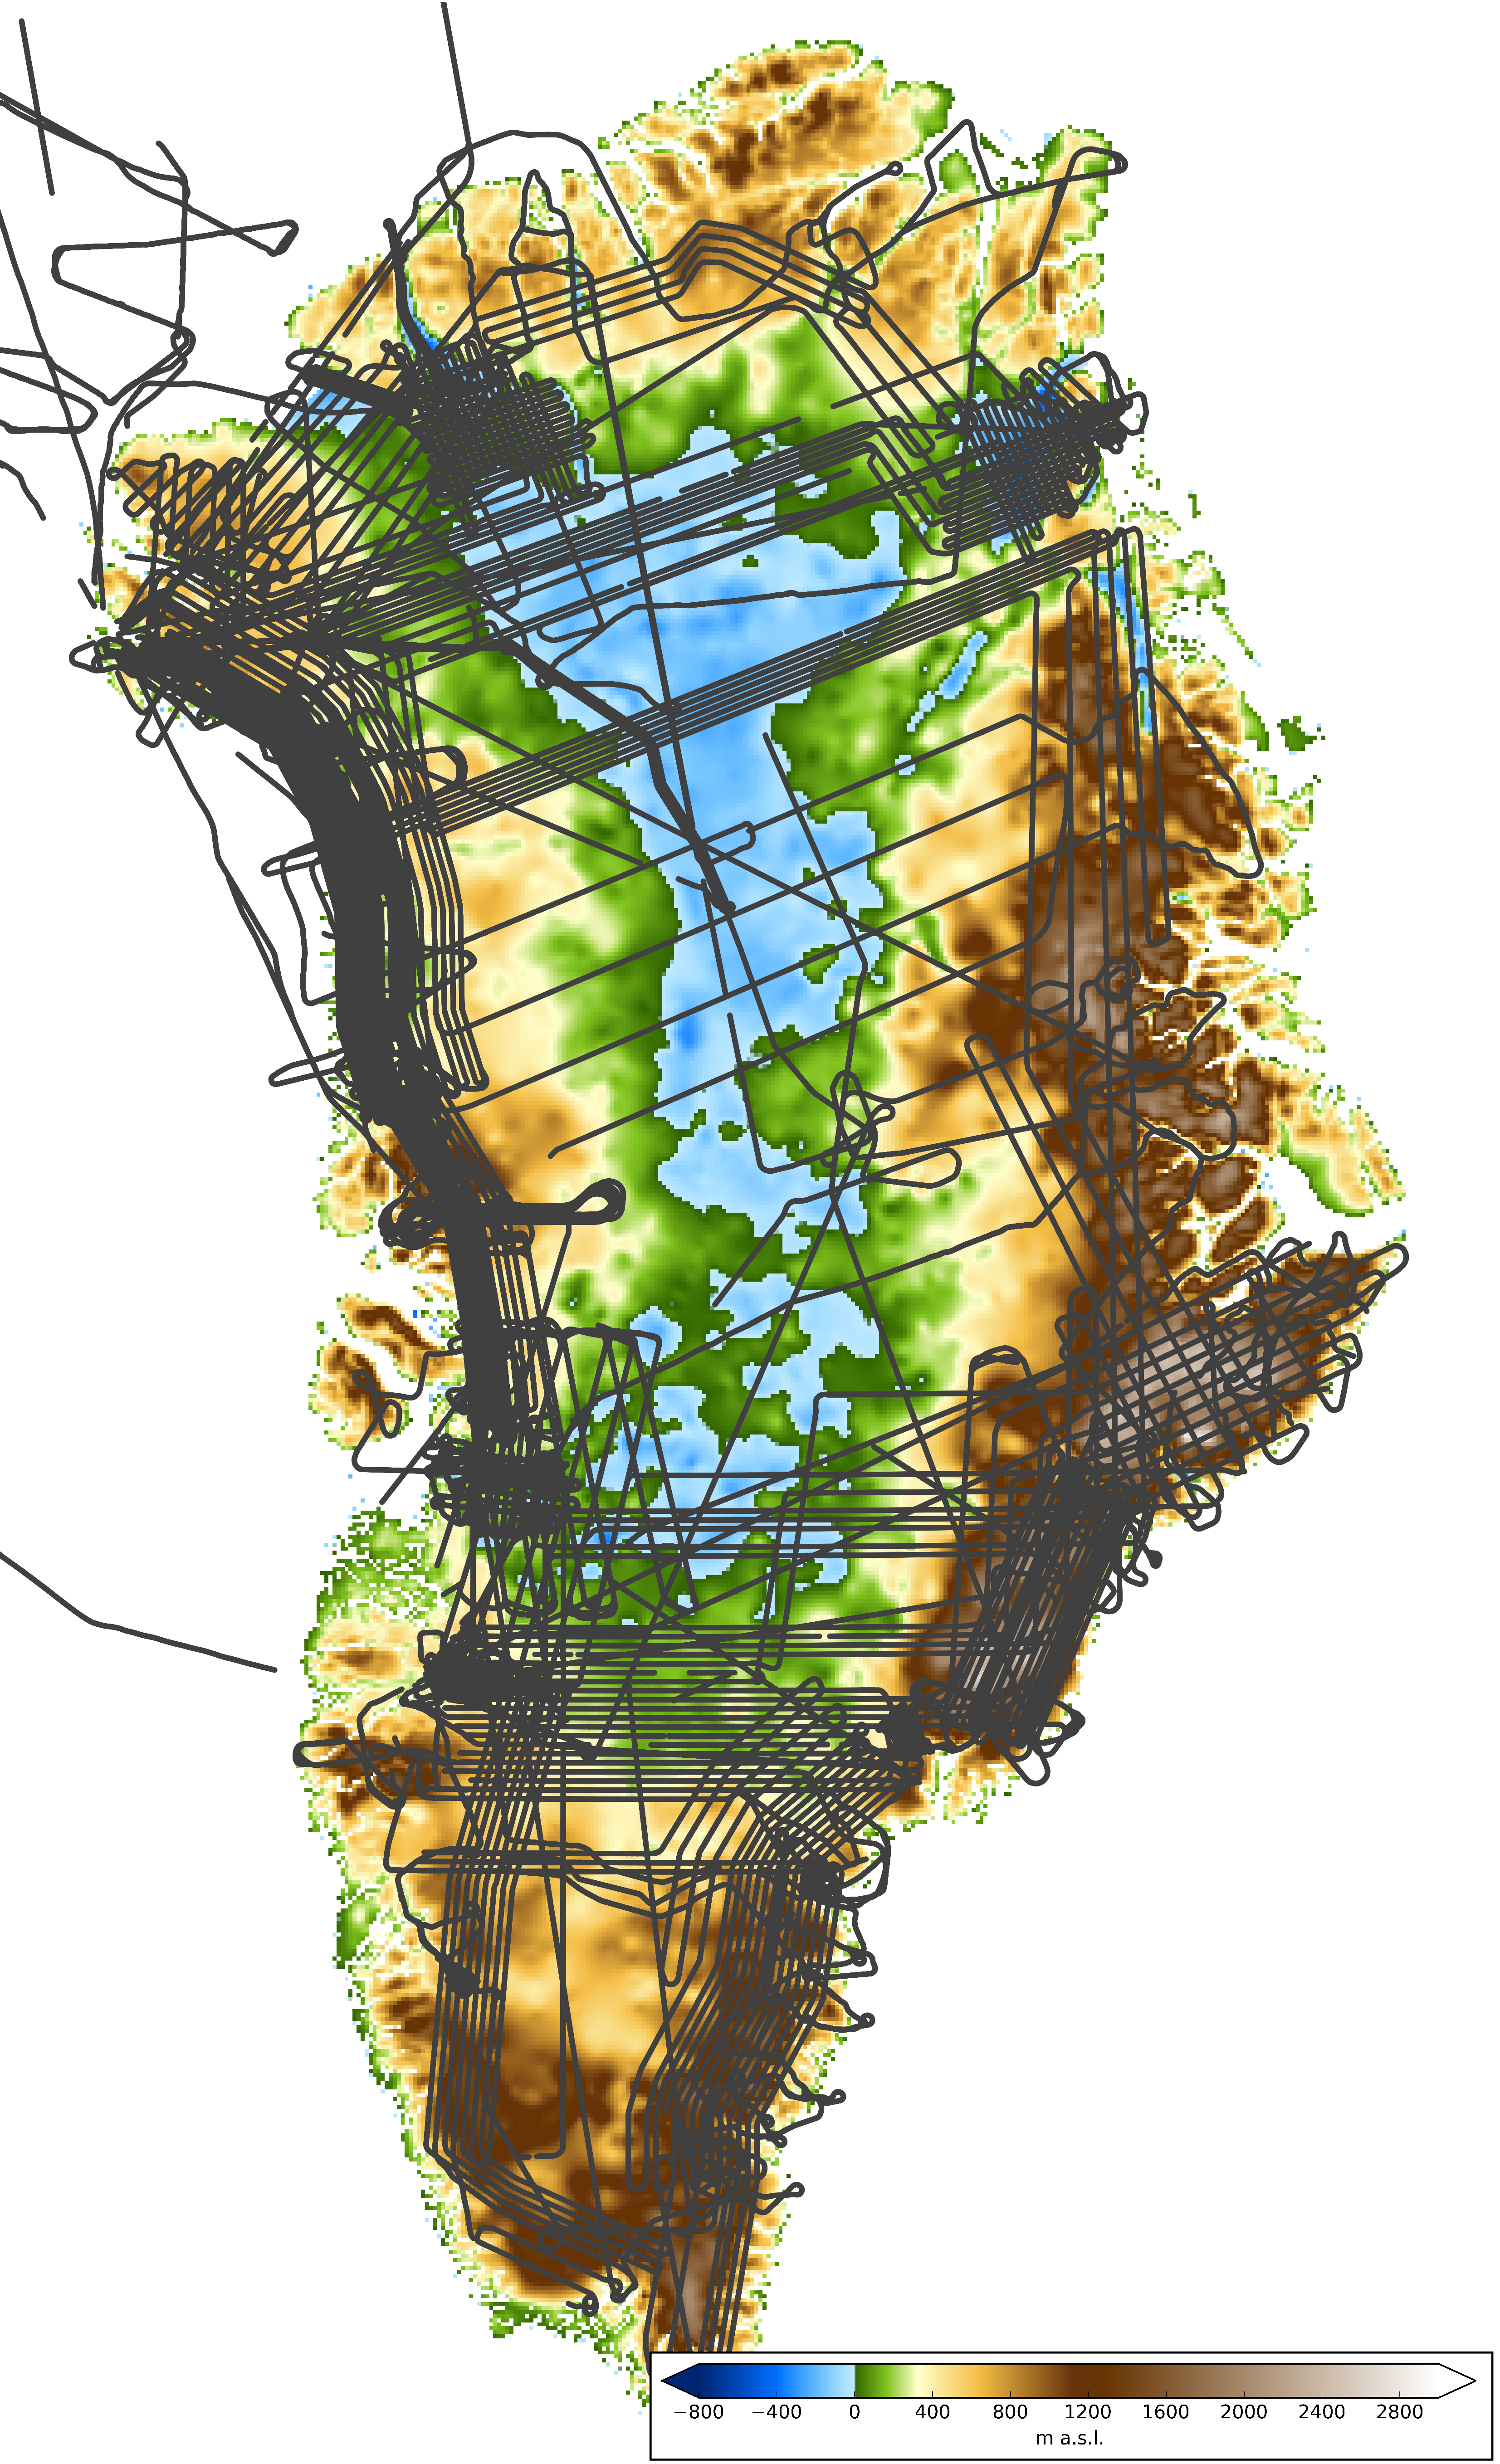
\includegraphics[height=8cm]{greenland-bed-old-oib}
    \end{figure}
  \end{columns}
\end{frame}

\begin{frame}{Zoom in to Jakobshavn Isbr{\ae}}
  \begin{figure}
    \small{old (2001) \hspace{5em} new (2014)}
    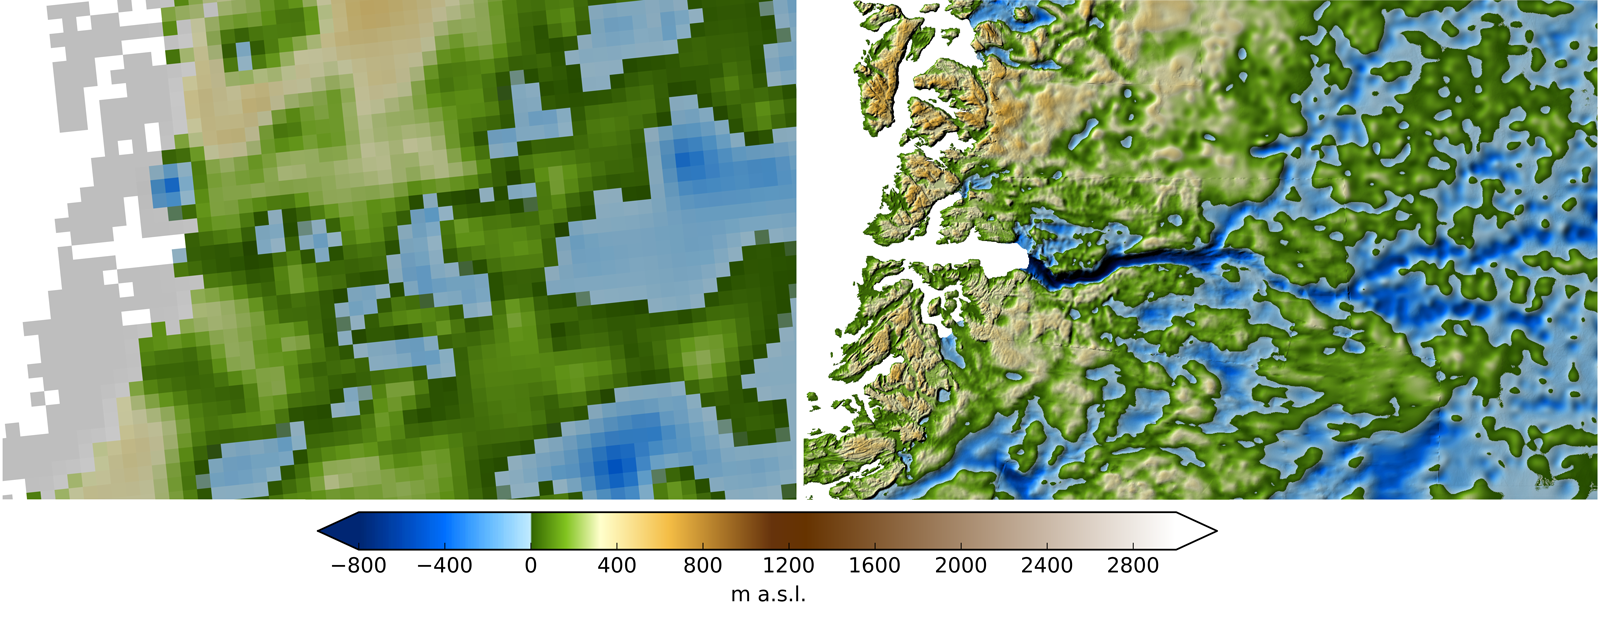
\includegraphics[width=12cm]{jako_bed}
 \end{figure}
\end{frame}


\begin{frame}{NASA Operation IceBridge}
  \begin{columns}
    \column[c]{8cm}
    \begin{figure}
      \small{old (2001) \hspace{4em} new (2014)}
      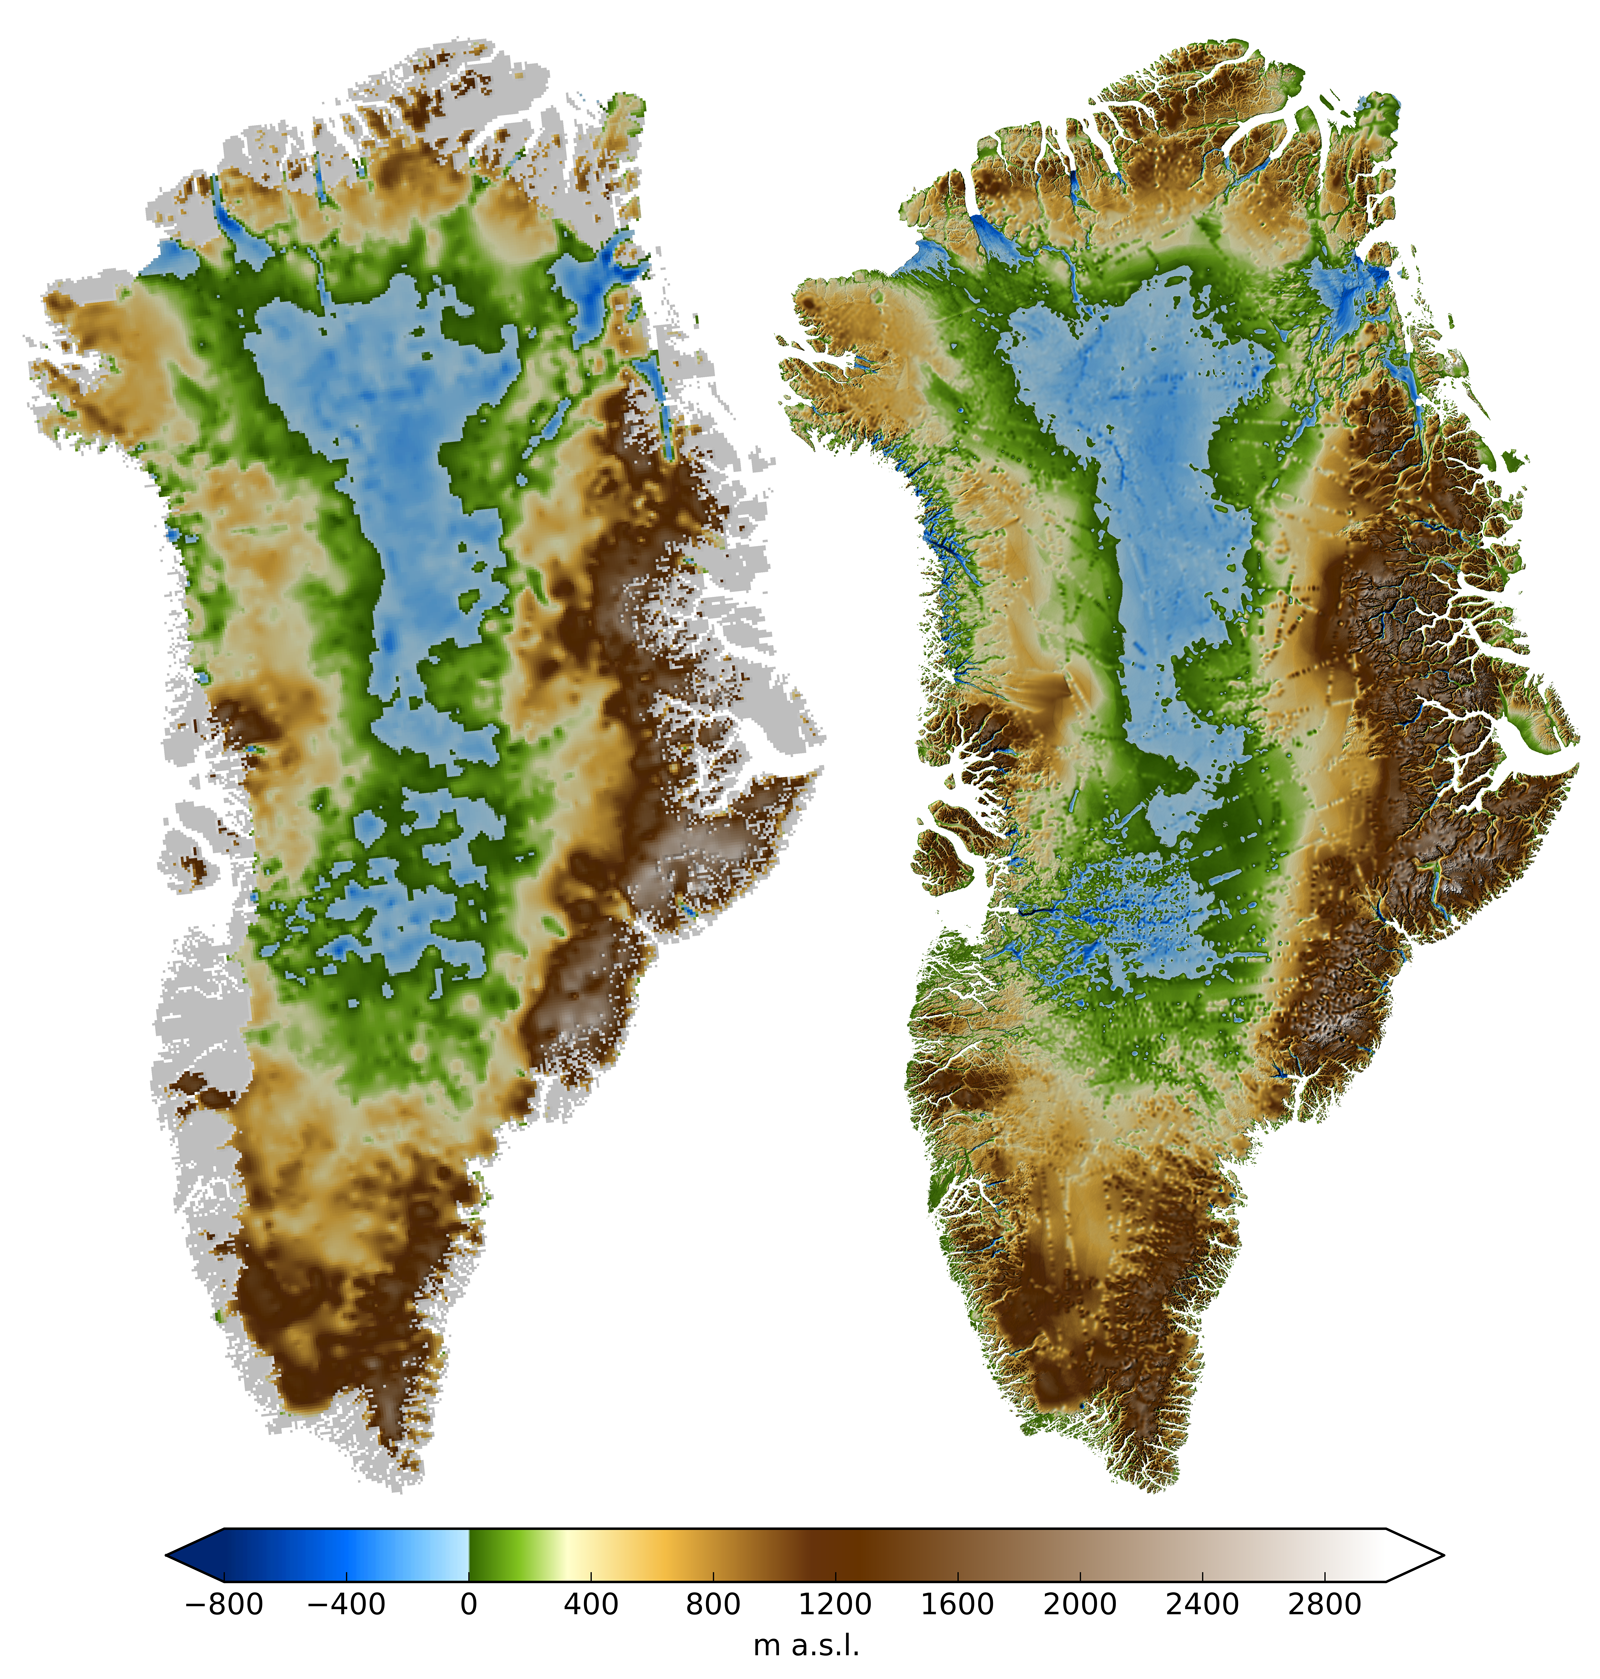
\includegraphics[height=7.5cm]{greenland_bed}
    \end{figure}
    \column[c]{4cm}
    \begin{itemize}
    \item from 5\,km to 150\,m horizontal grid resolution
    \end{itemize}
  \end{columns}
\end{frame}

\begin{frame}{NASA Operation IceBridge}
  \begin{figure}
    
\includegraphics[height=2.5cm]{nasa-logo} \qquad
    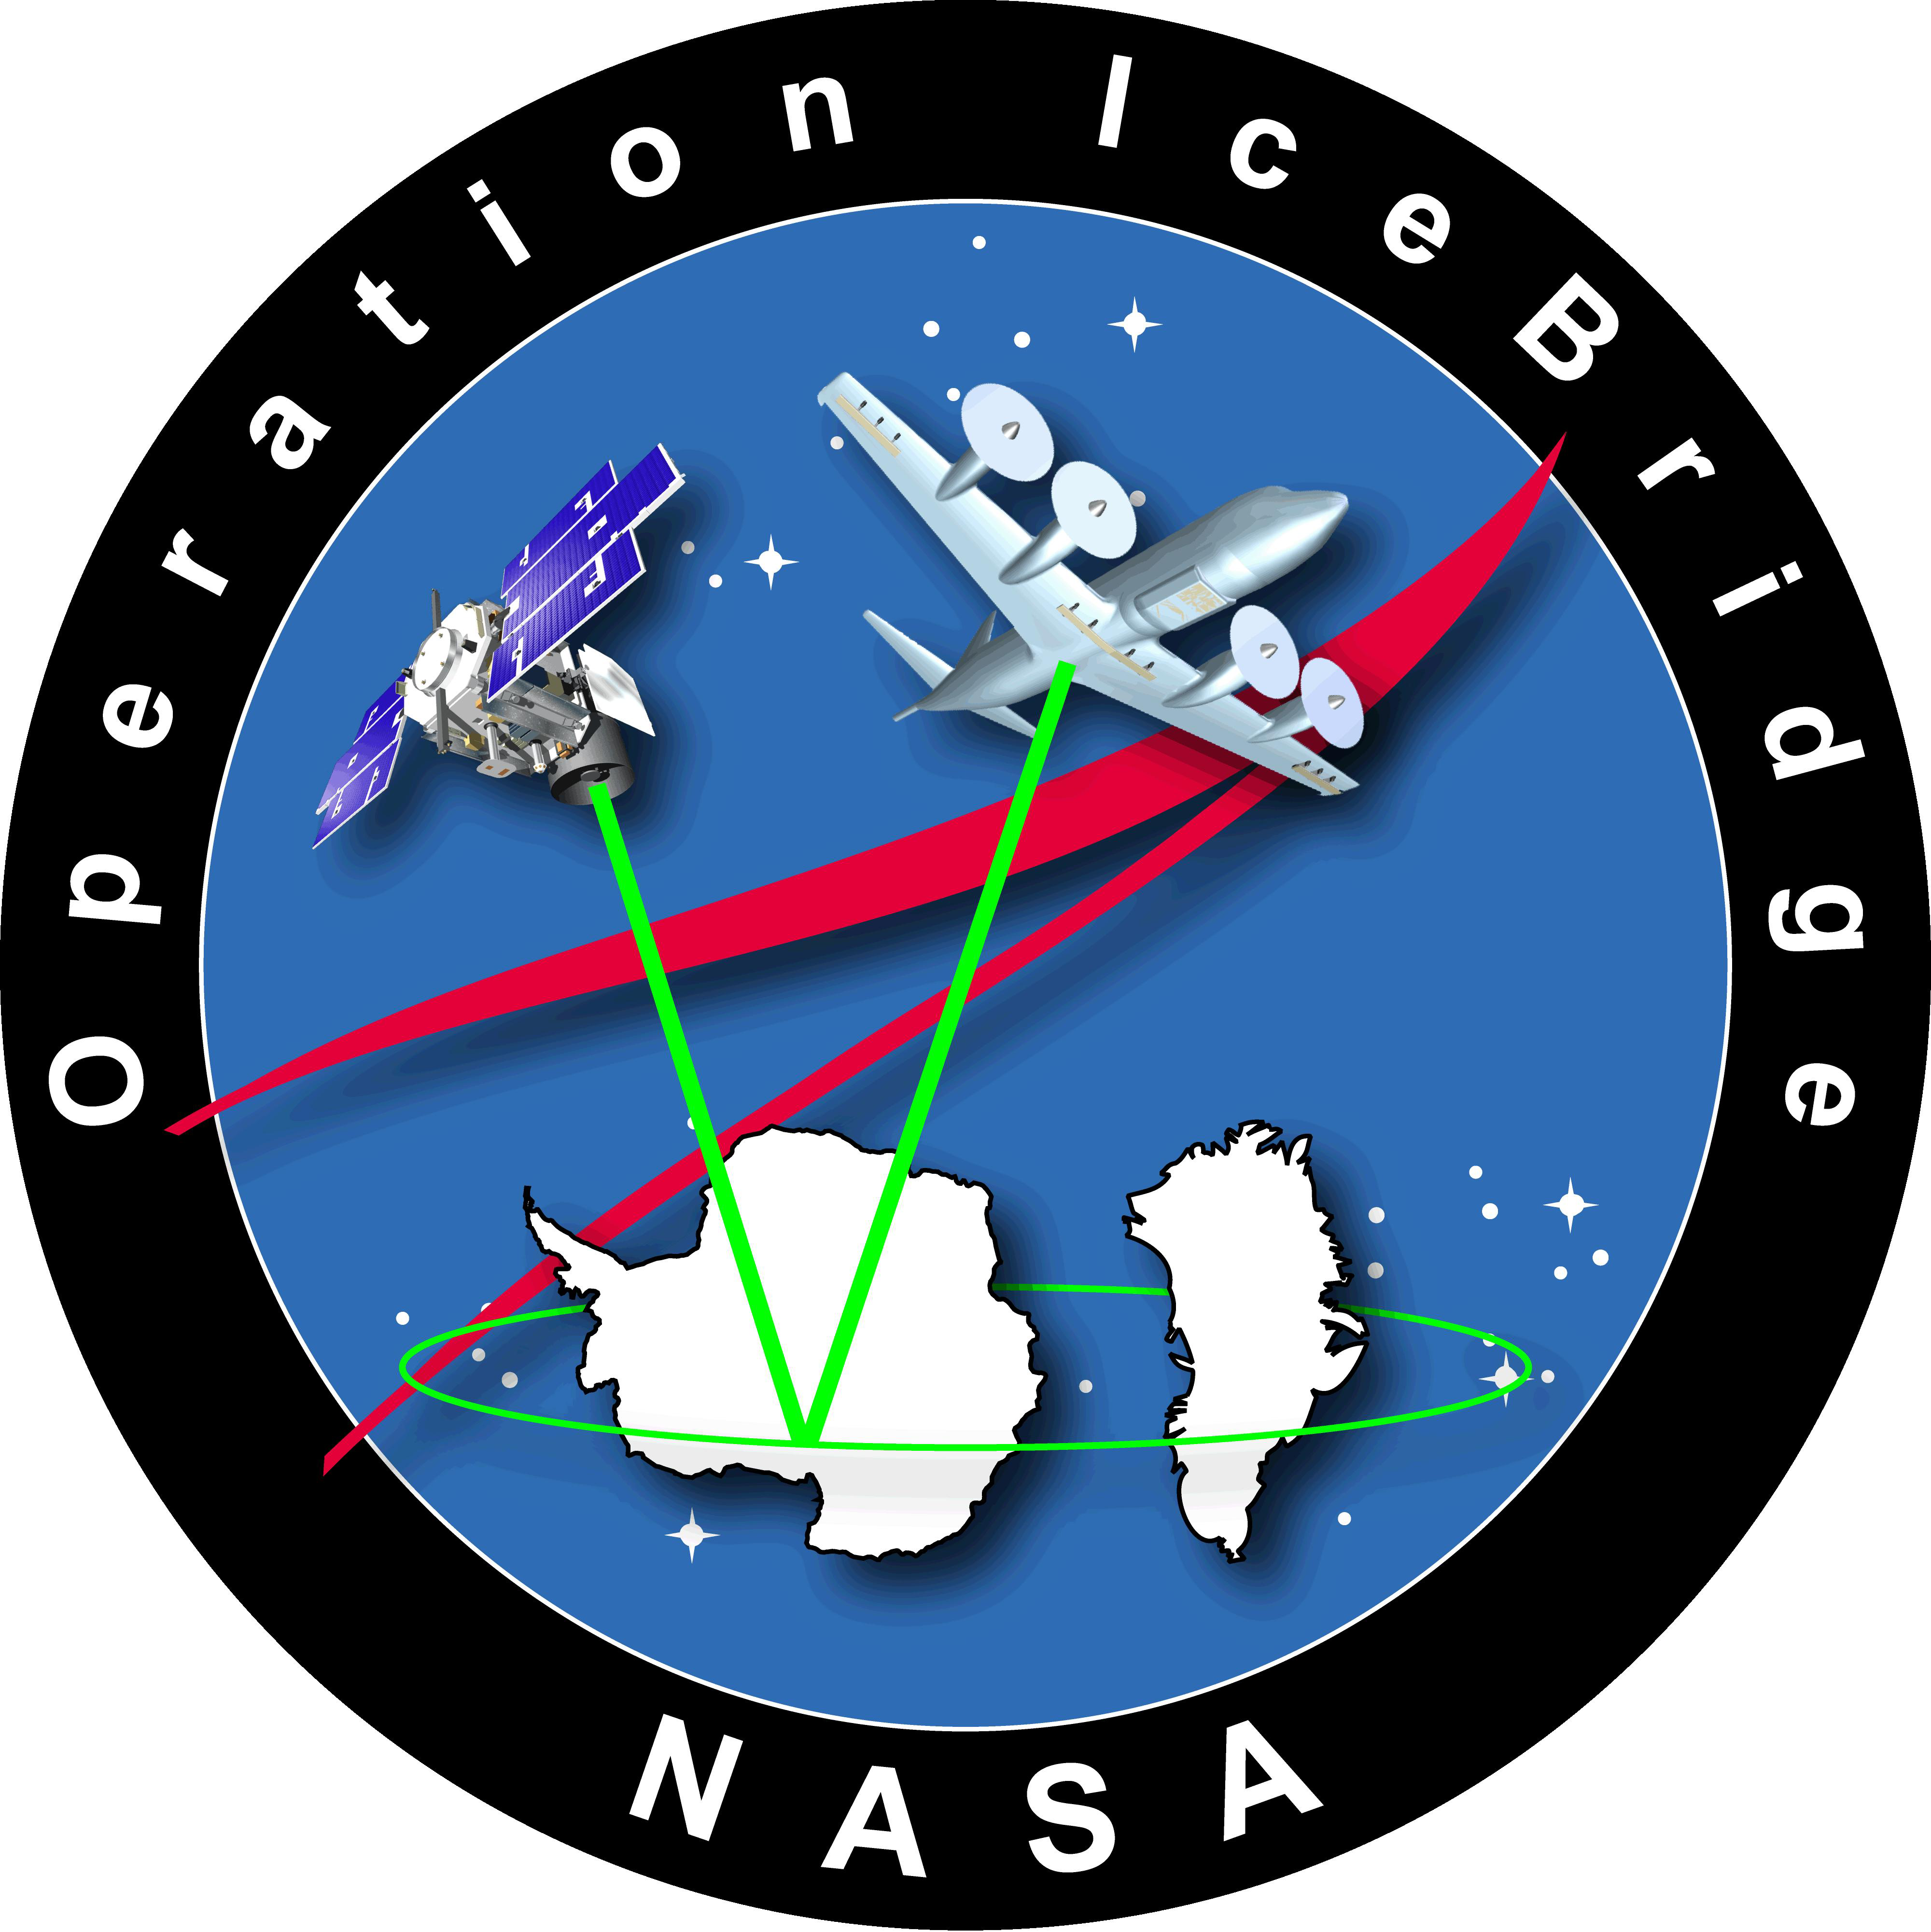
\includegraphics[height=2.5cm]{oib} \qquad
    \includegraphics[height=2.5cm]{1000-dollar-bills}
  \end{figure}
  \begin{itemize}
  \item do NASA's OIB million\$ really make ice sheet models better?
  \end{itemize}
  \note[item]{so the multi million dollar question is}
  \note[item]{does this investment pay off?}
\end{frame}


\begin{frame}{Observed flow speeds}
\vspace{-0.74em}
  \begin{columns}
    \column[c]{5cm}
    \begin{figure}
      \includegraphics[width=\textwidth]{greenland-obs-overview}
    \end{figure}
    \column[c]{5cm}
    \only<1>{Jakobshavn Isbr{\ae}}
    \includegraphics<1>[width=\textwidth]{jakobshavn-obs-nogate}
    \only<1>{\\ {} }
  \end{columns}
  \note[item]{let's look at JIB again}
  \note[item]{observations show strongly channelized flow}
  \note[item]{with high flow speeds in the center}
\end{frame}


\begin{frame}{Ice thickness and simulated flow speeds}
\vspace{-0.74em}
  \begin{columns}
    \column[c]{5cm}
    \begin{figure}
      \includegraphics<1-2>[width=\textwidth]{greenland-obs-basal-overview}
      \includegraphics<3-4>[width=\textwidth]{greenland-obs-basal-overview-mo14}
    \end{figure}
    \column[c]{5cm}
    \only<1,3>{Jakobshavn Isbr{\ae}}
    \only<2>{no fast flow}
    \only<4>{fast flow appears}
    \includegraphics<1>[width=\textwidth]{jakobshavn-bed-5000m-ba01}
    \includegraphics<2>[width=\textwidth]{jakobshavn-speed-exp-4500m-ba01}
    \includegraphics<3>[width=\textwidth]{jakobshavn-bed-mo14}
    \includegraphics<4>[width=\textwidth]{jakobshavn-speed-exp-600-v1.2-no-scale-no-gate}
    \only<1>{\\ 5\,km, old data set (2001)}
    \only<2,4>{\\ simulated surface speed}
    \only<3>{\\ 600\,m, new data set (2014)}
  \end{columns}
  \note<1>[item]{now let's do a simualulation with the old ice thickness data}
  \note<2>[item]{there isn't really any fast flow}
  \note<3>[item]{now use the new ice thickness}
  \note<4>[item]{and we get fast flow}
\end{frame}


\begin{frame}{Can we capture the present-day flow field?}
  \begin{figure}
    \includegraphics[height=7cm]{greenland-overview-3}
    \\ \scriptsize{Aschwanden, Fahnestock, Truffer (2016) \textit{Nature Communications}}
  \end{figure}
  \note[item]{first time capturing the flow field for the right reason}
  \note[item]{this is quite a break through in ice sheet modeling}
  \note[item]{though not a surprising one}
  \note[item]{it just confirms what students learn in glaciology 100:}
  \note[item]{ice flows downhill}
\end{frame}



\begin{frame}{Understanding the recent past}
  first high-resolution hindcast of the satellite era
    \begin{figure}
      \movie[showcontrols=true,loop,width=8cm]{\includegraphics[width=8cm]{jako_hindcast_frame000}}{jako_hindcast_hd.mov}
  \end{figure}
  \note[item]{now that we can capture the present-day flow patterns}
  \note[item]{reasonably well, we can add the temporal dimension}
\end{frame}


\begin{frame}{Next step: Vulnerability assessment}
  What has the future in stock?
    \begin{figure}
      \movie[showcontrols=true,autostart,loop,width=12cm]{\includegraphics[width=12cm]{jak_collapse_frame000}}{jak_collapse.mov}
  \end{figure}
\end{frame}


\begin{frame}{Summary}
  \begin{columns}[c]
    \begin{column}{2.25cm}
      \shadowimage[width=2cm]{plug}        
    \end{column}
    \begin{column}{10cm}
      ``pulling the plug'' (loss of floating tongue) causes outlet glaciers to speed up    
    \end{column}
  \end{columns}
  \begin{columns}[c]
    \begin{column}{2.25cm}
      \shadowimage[width=2cm]{jakobshavn-speed-exp-600-v1.2-no-scale-no-gate}
    \end{column}
    \begin{column}{10cm}
     outlet glacier flow is well captured where accurate ice thickness data are available (large return on investment)
    \end{column}
  \end{columns}
  \begin{columns}[c]
    \begin{column}{2.25cm}
      \shadowimage[width=2cm]{jako_hindcast_frame000}    
    \end{column}
    \begin{column}{10cm}
      initial efforts to simulate the recent past are promising    
    \end{column}
  \end{columns}
  \begin{columns}[c]
    \begin{column}{2.25cm}
      \shadowimage[width=2cm]{jak_collapse_frame_last}    
    \end{column}
    \begin{column}{10cm}
      how will Greenland look like in a 1000 years?
    \end{column}
  \end{columns}

\end{frame}

\begin{frame}{Acknowledgments}
  \begin{figure}
    \includegraphics[height=1.5cm]{nasa-logo}
    \includegraphics[height=1.5cm]{NSF_logo_color}
  \end{figure}
  
  \begin{columns}[c]
    \begin{column}{2cm}
      \shadowimage[height=1.75cm]{mark}    
    \end{column}
    \begin{column}{3cm}
      Mark Fahnestock
    \end{column}
    \begin{column}{2.cm}
      \shadowimage[height=1.75cm]{martin}    
    \end{column}
    \begin{column}{3.5cm}
      Martin Truffer
    \end{column}
  \end{columns}

  \begin{columns}[c]
    \vspace{-.5em}
    \begin{column}{2cm}
      \shadowimage[height=1.75cm]{ed}    
    \end{column}
    \begin{column}{3cm}
      Ed Bueler
    \end{column}
    \begin{column}{2cm}
      \shadowimage[height=1.75cm]{constantine}    
    \end{column}
    \begin{column}{3.5cm}
      Constantine Khroulev
    \end{column}
  \end{columns}
  \bigskip
  \begin{itemize}
    \item \ldots and the glacier's group
  \end{itemize}
\end{frame}

\begin{frame}[plain]
  \animategraphics[autoplay,keepaspectratio,loop]{0.5}{taku-}{1}{18}
\end{frame}

\end{document}
